% Options for packages loaded elsewhere
\PassOptionsToPackage{unicode}{hyperref}
\PassOptionsToPackage{hyphens}{url}
\PassOptionsToPackage{dvipsnames,svgnames,x11names}{xcolor}
\documentclass[
  11pt,
]{article}
\usepackage{xcolor}
\usepackage[a4paper,textwidth=160mm,textheight=232mm,top=31mm,hcentering,headsep=9mm,footskip=13mm]{geometry}
\usepackage{amsmath,amssymb}
\setcounter{secnumdepth}{5}
\usepackage{iftex}
\ifPDFTeX
  \usepackage[T1]{fontenc}
  \usepackage[utf8]{inputenc}
  \usepackage{textcomp} % provide euro and other symbols
\else % if luatex or xetex
  \usepackage{unicode-math} % this also loads fontspec
  \defaultfontfeatures{Scale=MatchLowercase}
  \defaultfontfeatures[\rmfamily]{Ligatures=TeX,Scale=1}
\fi
\usepackage{lmodern}
\ifPDFTeX\else
  % xetex/luatex font selection
\fi
% Use upquote if available, for straight quotes in verbatim environments
\IfFileExists{upquote.sty}{\usepackage{upquote}}{}
\IfFileExists{microtype.sty}{% use microtype if available
  \usepackage[]{microtype}
  \UseMicrotypeSet[protrusion]{basicmath} % disable protrusion for tt fonts
}{}
\usepackage{graphicx}
\makeatletter
\newsavebox\pandoc@box
\newcommand*\pandocbounded[1]{% scales image to fit in text height/width
  \sbox\pandoc@box{#1}%
  \Gscale@div\@tempa{\textheight}{\dimexpr\ht\pandoc@box+\dp\pandoc@box\relax}%
  \Gscale@div\@tempb{\linewidth}{\wd\pandoc@box}%
  \ifdim\@tempb\p@<\@tempa\p@\let\@tempa\@tempb\fi% select the smaller of both
  \ifdim\@tempa\p@<\p@\scalebox{\@tempa}{\usebox\pandoc@box}%
  \else\usebox{\pandoc@box}%
  \fi%
}
% Set default figure placement to htbp
\def\fps@figure{htbp}
\makeatother
% definitions for citeproc citations
\NewDocumentCommand\citeproctext{}{}
\NewDocumentCommand\citeproc{mm}{%
  \begingroup\def\citeproctext{#2}\cite{#1}\endgroup}
\makeatletter
 % allow citations to break across lines
 \let\@cite@ofmt\@firstofone
 % avoid brackets around text for \cite:
 \def\@biblabel#1{}
 \def\@cite#1#2{{#1\if@tempswa , #2\fi}}
\makeatother
\newlength{\cslhangindent}
\setlength{\cslhangindent}{1.5em}
\newlength{\csllabelwidth}
\setlength{\csllabelwidth}{3em}
\newenvironment{CSLReferences}[2] % #1 hanging-indent, #2 entry-spacing
 {\begin{list}{}{%
  \setlength{\itemindent}{0pt}
  \setlength{\leftmargin}{0pt}
  \setlength{\parsep}{0pt}
  % turn on hanging indent if param 1 is 1
  \ifodd #1
   \setlength{\leftmargin}{\cslhangindent}
   \setlength{\itemindent}{-1\cslhangindent}
  \fi
  % set entry spacing
  \setlength{\itemsep}{#2\baselineskip}}}
 {\end{list}}
\usepackage{calc}
\newcommand{\CSLBlock}[1]{\hfill\break\parbox[t]{\linewidth}{\strut\ignorespaces#1\strut}}
\newcommand{\CSLLeftMargin}[1]{\parbox[t]{\csllabelwidth}{\strut#1\strut}}
\newcommand{\CSLRightInline}[1]{\parbox[t]{\linewidth - \csllabelwidth}{\strut#1\strut}}
\newcommand{\CSLIndent}[1]{\hspace{\cslhangindent}#1}
\setlength{\emergencystretch}{3em} % prevent overfull lines
\providecommand{\tightlist}{%
  \setlength{\itemsep}{0pt}\setlength{\parskip}{0pt}}
% =====================================================================
%  NeedleFinder 2026 -- PMB manuscript, print edition
%  Book-style typography: EB Garamond + Garamond-Math, A4, 120 mm measure,
%  floats breaking 20 mm into each margin, small-caps apparatus.
%  Compiled with tectonic (XeTeX); unicode-math/fontspec are loaded by pandoc.
% =====================================================================

% ---------- Colour (one accent: Okabe-Ito vermilion) -----------------
\usepackage{xcolor}
\usepackage{colortbl}
\definecolor{nfink}{HTML}{1F1C18}       % warm near-black for text
\definecolor{nfgrey}{HTML}{5E5850}      % secondary text (captions, notes)
\definecolor{nfrule}{HTML}{8C857B}
\definecolor{nfours}{HTML}{D55E00}      % accent: Okabe-Ito vermilion
\definecolor{nfaccent}{HTML}{B34E00}    % accent at text-safe contrast
\definecolor{nfst0}{HTML}{E69F00}
\definecolor{nfst1}{HTML}{0072B2}
\definecolor{nfst2}{HTML}{009E73}
\definecolor{nfst0tint}{HTML}{F7ECCC}
\definecolor{nfst1tint}{HTML}{CCE3F0}
\definecolor{nfst2tint}{HTML}{CCECE3}
\definecolor{nfrow}{HTML}{FBF1E7}       % restrained vermilion tint ("ours")
\definecolor{nfourstext}{HTML}{9E4400}
\definecolor{nfctrow}{HTML}{F1EFEB}     % warm grey tint (CT studies)
\definecolor{ctrow}{HTML}{F1EFEB}
\color{nfink}

% ---------- Fonts -----------------------------------------------------
% EB Garamond (Duffner/Pardo) for text, old-style proportional figures in
% prose; Garamond-Math for mathematics with digits and the decimal point
% taken from the text face so that numbers read identically in and out of
% math. Tables switch to tabular lining figures (\nftabfont + \nflinmath).
\defaultfontfeatures{Ligatures=TeX}
\setmainfont{EBGaramond}[
  Extension=.otf,
  UprightFont=*-Regular, ItalicFont=*-Italic,
  BoldFont=*-SemiBold, BoldItalicFont=*-SemiBoldItalic,
  Numbers={OldStyle,Proportional},
  Ligatures={TeX,Common},
  SmallCapsFeatures={Letters=SmallCaps, LetterSpace=4}]
\newfontfamily\nfcapsfont{EBGaramond}[
  Extension=.otf, UprightFont=*-Regular, ItalicFont=*-Italic,
  BoldFont=*-SemiBold,
  Letters={SmallCaps,UppercaseSmallCaps}, LetterSpace=8,
  Numbers={OldStyle,Proportional}]
\newfontfamily\nftabfont{EBGaramond}[
  Extension=.otf, UprightFont=*-Regular, ItalicFont=*-Italic,
  BoldFont=*-SemiBold, BoldItalicFont=*-SemiBoldItalic,
  Numbers={Lining,Monospaced}]
\setmonofont{IBMPlexMono}[Extension=.otf, Scale=0.84, HyphenChar=None,
  UprightFont=*-Regular, ItalicFont=*-Italic,
  BoldFont=*-Medium, BoldItalicFont=*-MediumItalic]
% Code identifiers (NeedleSliceMPNN, TipAwareBundleGraphTransformer, ...) may
% break without a hyphen at a lower->upper case transition or after "_".
\newXeTeXintercharclass\nfLower
\newXeTeXintercharclass\nfUpper
\newXeTeXintercharclass\nfUnder
\count255=`a \loop\XeTeXcharclass\count255=\nfLower\ifnum\count255<`z\advance\count255 by 1\repeat
\count255=`A \loop\XeTeXcharclass\count255=\nfUpper\ifnum\count255<`Z\advance\count255 by 1\repeat
\XeTeXcharclass`_=\nfUnder
\XeTeXinterchartoks\nfLower\nfUpper={\penalty200\hskip0pt\relax}
\XeTeXinterchartoks\nfUnder\nfUpper={\penalty200\hskip0pt\relax}
\XeTeXinterchartoks\nfUnder\nfLower={\penalty200\hskip0pt\relax}
\let\nforigtexttt\texttt
\renewcommand{\texttt}[1]{\nforigtexttt{\XeTeXinterchartokenstate=1 #1}}
\setmathfont{Garamond-Math.otf}
\setmathfont{EBGaramond-Regular.otf}[range={up/num,"2E}, Numbers={OldStyle,Proportional}]
% In tables, math digits switch to tabular lining figures as well.
\makeatletter
{\nftabfont\xdef\nf@tabfamily{\f@family}}
\DeclareSymbolFont{nflin}{TU}{\nf@tabfamily}{m}{n}
\def\nf@set#1{\Umathcode`#1=0 \symnflin `#1\relax}
\newcommand\nflinmath{\@tfor\nf@d:=0123456789.\do{\expandafter\nf@set\nf@d}}
\makeatother
\newcommand{\nfcaps}[1]{{\nfcapsfont #1}}

% ---------- Paragraphs, spacing, widows ------------------------------
\linespread{1.06}
\setlength{\parindent}{1.25em}
\setlength{\parskip}{0pt}
\setlength{\emergencystretch}{2.5em}
\tolerance=400 \pretolerance=150
\widowpenalty=10000 \clubpenalty=10000 \displaywidowpenalty=10000
\brokenpenalty=4000
\raggedbottom
% Under \raggedbottom every break has zero badness, so the default -300
% \@secpenalty makes any section start the "best" break and pages end early
% (e.g. before References). Neutralise it; headings still never strand.
\makeatletter\@secpenalty=0\makeatother
\frenchspacing
% camel-case names are otherwise unhyphenatable and leave loose lines
\hyphenation{Needle-Finder}
% let long URLs stretch a little inside the measure
\AtBeginDocument{\Urlmuskip=0mu plus 1.5mu\relax}
\microtypesetup{protrusion=true, tracking=false}
\usepackage{enumitem}
\setlist{itemsep=0.25\baselineskip, topsep=0.45\baselineskip, parsep=0pt}
\setlist[enumerate]{leftmargin=1.6em, label=\arabic*.}
\setlist[itemize]{leftmargin=1.4em, label=\textcolor{nfgrey}{\textendash}}

% ---------- Running heads and folios ----------------------------------
\usepackage{fancyhdr}
\pagestyle{fancy}
\fancyhf{}
\renewcommand{\headrulewidth}{0pt}
\renewcommand{\footrulewidth}{0pt}
\fancyhead[L]{\nfcaps{\footnotesize Pernelle et al.}}
\fancyhead[R]{\footnotesize\itshape Sub-millimeter 3D catheter reconstruction in MR-guided brachytherapy}
\fancyfoot[C]{\small\thepage}
\fancypagestyle{plain}{\fancyhf{}\fancyfoot[C]{\small\thepage}}
\setlength{\headheight}{14pt}
\fancyhfoffset[L,R]{-20mm}

% ---------- Section headings: hanging numbers in the margin -----------
\usepackage[explicit]{titlesec}
\newlength{\nfhang}\setlength{\nfhang}{1.6em}
\titleformat{\section}[block]
  {\normalsize}
  {\llap{\textcolor{nfours}{\thesection}\hspace{\nfhang}}}{0pt}
  {\nfcaps{#1}}
\titleformat{name=\section,numberless}[block]{\normalsize}{}{0pt}{\nfcaps{#1}}
\titleformat{\subsection}[block]
  {\normalsize\itshape}
  {\llap{\upshape\textcolor{nfours}{\thesubsection}\hspace{\nfhang}}}{0pt}
  {#1}
\titleformat{\subsubsection}[runin]
  {\normalsize\itshape}
  {\llap{\upshape\textcolor{nfours}{\thesubsubsection}\hspace{\nfhang}}}{0pt}
  {#1.}
\titlespacing*{\section}{0pt}{2.2\baselineskip plus 0.4\baselineskip minus 0.2\baselineskip}{0.9\baselineskip}
\titlespacing*{name=\section,numberless}{0pt}{1.5\baselineskip plus 0.3\baselineskip minus 0.2\baselineskip}{0.55\baselineskip}
\titlespacing*{\subsection}{0pt}{1.3\baselineskip plus 0.3\baselineskip minus 0.1\baselineskip}{0.5\baselineskip}
\titlespacing*{\subsubsection}{0pt}{0.9\baselineskip plus 0.2\baselineskip}{0.6em}

% ---------- Title page ------------------------------------------------
\makeatletter
\renewcommand{\maketitle}{%
  \thispagestyle{plain}%
  \begingroup
  \def\and{ }%
  \null\vspace*{-1.5\baselineskip}%
  {\raggedright
   {\nfcaps{\footnotesize Research paper}\hfill\nfcaps{\footnotesize Physics in Medicine \& Biology \textperiodcentered{} Manuscript}\par}%
   \vspace{0.35\baselineskip}%
   {\color{nfrule}\rule{\linewidth}{0.4pt}\par}%
   \vspace{2.2\baselineskip}%
   {\fontsize{21}{25.5}\selectfont\@title\par}%
   \vspace{1.4\baselineskip}%
   {\large\@author\par}%
   \vspace{0.5\baselineskip}%
   {\small\itshape\color{nfgrey}\@date\par}%
  }%
  \vspace{2.2\baselineskip}%
  \endgroup}
\makeatother
\renewenvironment{abstract}
  {\par\noindent{\small\nfcaps{Abstract}}\par\vspace{0.4\baselineskip}%
   \begingroup\small\setlength{\parindent}{0pt}\setlength{\parskip}{0.45\baselineskip}}
  {\par\endgroup
   \vspace{0.9\baselineskip}%
   \noindent{\color{nfrule}\rule{\linewidth}{0.4pt}}\par\vspace{0.4\baselineskip}}

% ---------- Tables: booktabs with hairlines ---------------------------
\usepackage{booktabs,tabularx,threeparttable,multirow,makecell,array,etoolbox}
\usepackage{changepage}
\setlength{\heavyrulewidth}{0.7pt}
\setlength{\lightrulewidth}{0.35pt}
\setlength{\cmidrulewidth}{0.3pt}
\setlength{\aboverulesep}{0.5ex}
\setlength{\belowrulesep}{0.6ex}
\setlength{\tabcolsep}{5.2pt}
\renewcommand{\arraystretch}{1.12}
\AtBeginEnvironment{tabular}{\nftabfont\nflinmath}
\AtBeginEnvironment{tablenotes}{\nftabfont\nflinmath\color{nfgrey}}
\newcommand{\best}[1]{\textbf{#1}}
\newcommand{\second}[1]{{\setbox0\hbox{#1}\rlap{\color{nfink}\rule[-0.32ex]{\wd0}{0.35pt}}\box0}}
\newcommand{\TBD}{\textcolor{red}{\textbf{TBD}}}
\newcommand{\rep}{\textsuperscript{r}}
% "ours" rows: a restrained tint plus a vermilion mark in the left gutter
\newcommand{\nfmark}{\llap{\textcolor{nfours}{\rule[-0.45ex]{1.1pt}{2.35ex}}\hspace{3.5pt}}}
\newcommand{\oursrow}{\rowcolor{nfrow}\nfmark}
\newcommand{\ctrow}{\rowcolor{nfctrow}}
\newcommand{\NF}{\textbf{NeedleFinder\,2026}}
\newcommand{\Eshaft}{$E_{\mathrm{shaft}}$}
\newcommand{\Etip}{$E_{\mathrm{tip}}$}
\newcommand{\Davg}{$D_{\mathrm{avg}}$}
\newcommand{\HD}{$\mathrm{HD}$}
\newcolumntype{L}{>{\raggedright\arraybackslash}l}
\newcolumntype{R}{>{\raggedleft\arraybackslash}r}
\newcolumntype{C}{>{\centering\arraybackslash}c}
\newcolumntype{Y}{>{\raggedright\arraybackslash}X}

% ---------- Measure: 120 mm text inside a 160 mm block ----------------
% geometry sets a 160 mm text block (the natural width of floats). Running
% text is set 20 mm in from each side by one document-wide list, so the
% measure is 120 mm (~68 characters) while figures and tables, which reset
% to \columnwidth, break out 20 mm into each margin.
\newlength{\nfbreak}\setlength{\nfbreak}{20mm}
\AtBeginDocument{\begin{adjustwidth}{\nfbreak}{\nfbreak}}
\AtEndDocument{\end{adjustwidth}}

% ---------- Captions: small type, small-caps label hung in the margin --
\usepackage{caption}
\DeclareCaptionLabelFormat{nfsc}{\nfcaps{#1~#2}}
\DeclareCaptionFormat{nfhang}{\noindent\llap{#1\hspace{0.9em}}#3}
\captionsetup{format=plain, font={small}, labelfont={}, textfont={},
  labelformat=nfsc, labelsep=quad, justification=justified,
  singlelinecheck=false, skip=7pt}
% figure captions keep to the text measure, label hung to the left
\captionsetup[figure]{format=nfhang, margin={\nfbreak,\nfbreak}, skip=9pt}
% table captions sit above the table and run the table's width
\captionsetup[table]{position=top, skip=5pt}
\setlength{\abovecaptionskip}{7pt}

\usepackage{placeins}
\usepackage{float}
\renewcommand{\topfraction}{0.92}
\renewcommand{\bottomfraction}{0.6}
\renewcommand{\textfraction}{0.08}
\renewcommand{\floatpagefraction}{0.75}
\setcounter{topnumber}{3}
\setcounter{bottomnumber}{1}
\setcounter{totalnumber}{4}
\setlength{\floatsep}{1.6\baselineskip plus 0.4\baselineskip minus 0.2\baselineskip}
\setlength{\textfloatsep}{1.8\baselineskip plus 0.4\baselineskip minus 0.3\baselineskip}
\setlength{\intextsep}{1.6\baselineskip plus 0.4\baselineskip minus 0.2\baselineskip}
\usepackage{rotating}
\makeatletter   % float pages: stack from the top rather than centring vertically
\setlength{\@fptop}{0pt}
\setlength{\@fpsep}{2\baselineskip plus 1fil}
\setlength{\@fpbot}{0pt plus 1fil}
\makeatother

% ---------- Bibliography ----------------------------------------------
\AtBeginEnvironment{CSLReferences}{\small\raggedright\setlength{\cslhangindent}{1.5em}}

% ---------- Links -----------------------------------------------------
% Ink-coloured citations, accent for cross-references: set through pandoc's
% colorlinks/linkcolor/citecolor/urlcolor variables in build_paper.sh, so that
% hyperref receives colorlinks once (no "already been used" warning).
\usepackage{bookmark}
\IfFileExists{xurl.sty}{\usepackage{xurl}}{} % add URL line breaks if available
\urlstyle{same}
\hypersetup{
  pdftitle={NeedleFinder 2026: Sub-Millimeter Catheter Reconstruction on MRI for Interstitial Gynecologic Brachytherapy in Seconds},
  pdfauthor={Guillaume Pernelle, Paolo Zaffino, Lauren Barber, Alireza Mehrtash,; Christiane Yeung, Tina Kapur, and Collaborators},
  colorlinks=true,
  linkcolor={nfaccent},
  filecolor={Maroon},
  citecolor={nfink},
  urlcolor={nfaccent},
  pdfcreator={LaTeX via pandoc}}

\title{NeedleFinder 2026: Sub-Millimeter Catheter Reconstruction on MRI
for Interstitial Gynecologic Brachytherapy in Seconds}
\author{Guillaume Pernelle, Paolo Zaffino, Lauren Barber, Alireza
Mehrtash, \and Christiane Yeung, Tina Kapur, and Collaborators}
\date{October 2026 (Target Journal: \emph{Physics in Medicine \&
Biology})}

\begin{document}
\maketitle
\begin{abstract}
\textbf{Objective.} Interstitial gynecologic brachytherapy planned on
MRI alone requires locating 15 to 30 thin plastic catheters on 3T
T2-weighted images. Tracing them by hand takes tens of minutes while the
patient is under anesthesia. Automatic methods based on voxel
segmentation break catheters into fragments and mistake blood vessels
for catheters. We set out to make catheter reconstruction automatic,
accurate to below a millimeter, and fast enough to run during the
procedure.

\textbf{Approach.} NeedleFinder 2026 works in three stages. Stage 0
computes an analytical 3D circular dark-core symmetry prior (\(S_0\))
and a 100\% reference-free, tilt-safe axial field-of-view bound
(\texttt{k\_lim\_auto}) that eliminates all 42 in-FOV template-base
truncations while preserving 100.0\% of in-FOV catheter depth (99.65\%
of unclipped VTK \(z\)-span). Stage 1 is a native-resolution 3D residual
U-Net (\texttt{NeedleUNet3D}) self-supervised pre-trained on 51 strictly
external pelvic T2W MRI volumes from 50 distinct subjects (combining 3D
masked autoencoding with synthetic 3D susceptibility-tube pretext
learning against real anatomical hard negatives) and trained with
multi-rater supervision (\texttt{CY+HT} plus consensus-fused and
soft-weighted \texttt{LB/AMe} traces on outer-training folds), 5-fold
inner ensembling, and 4-view 3D test-time augmentation. Stage 2 traces
candidate trajectories with native bidirectional Kalman tracking, a
4-layer triplet message-passing network, and collinear split-fragment
stitching (\texttt{102} stitched full-length trajectories), scores the
whole implant bundle with a graph transformer pre-trained on 300
simulated bundles (\texttt{SynthBrachy3T}), and refines each distal tip
with a dedicated 91-step (\texttt{0.5\ mm} sub-slice Z-interpolated)
22-channel 3-block dilated 1D ResNet + 4-head self-attention axial
localizer (\texttt{Dedicated1DTipLocalizer}) equipped with strictly
nested split-conformal 3D tip uncertainty intervals. We evaluated the
pipeline on 54 clinical 3T MRI scans (1,063 catheters) under a strictly
nested \(5 \times 5\) patient-level cross-validation protocol
(\texttt{25} inner models, zero outer-test leakage), against three
published methods, across all 40 dual-traced scans via Grubbs'
three-cornered-hat and one-sided non-inferiority tests, in AAPM TG-43U1
HDR \(^{192}\text{Ir}\) dosimetric simulations, on 48 public needle-free
pelvic MRI scans, and zero-shot across prostate MRI
(\texttt{Case\ 100}), secondary MRI sequences (\texttt{3D\ wbSSFP},
\texttt{2D\ AX\ TSE\ T2}), 23 serial 4D insertion scans
(\texttt{Cases\ 68–71}), and 40 post-implant pelvic CT volumes (38
paired with benchmark MRI patients).

\textbf{Main results.} At the default threshold \(\tau = 50\%\),
NeedleFinder 2026 detected 91.4\% of all 1,063 catheters
(\texttt{972/1,063}) with 86.9\% precision (\texttt{972/1,118}) and
89.1\% F1 (\texttt{89.1\%} F1 and \texttt{92.3\%} recall with
\(5 \times 5\) inner-OOF cross-fit; \texttt{89.4\%} F1 at
\(\tau = 55\%\); \texttt{93.6\%} whole-cohort recall at
\(\tau = 35\%\)), outperforming our 2019-style 3D U-Net (\texttt{83.1\%}
F1, \(p = 1.1 \times 10^{-5}\)), a native-resolution clDice ResUNet
(\texttt{38.7\%} F1, \(p = 5.2 \times 10^{-10}\)), and a 2026-style
structure-aware tracker (\texttt{54.2\%} F1,
\(p = 3.0 \times 10^{-10}\)). On the 759 long interstitial shafts, it
achieved 91.3\% recall (\texttt{92.5\%} inner-OOF cross-fit;
\texttt{94.7\%} long-shaft recall at \(\tau = 35\%\)) and 90.0\%
\(F1_{\text{adj}}\) (\texttt{90.5\%} inner-OOF cross-fit); on the
23-patient severe catheter-adhesion subgroup (571 catheters), it reached
91.3\% F1 (\texttt{91.8\%} inner-OOF cross-fit). The in-plane shaft
error was \(0.59 \pm 0.40\) mm (\(0.47\) mm median, \(1.37\) mm P95),
and the 1D axial tip localizer cut 3D distal tip error to \(6.23\) mm
mean (\(2.27\) mm median, \(27.27\) mm P95; \(58.7\%\) within \(\le 3\)
mm; \(98.8\%\) of total squared 3D tip error longitudinal along the
shaft). Across all 40 dual-traced scans (\(n=432\) three-way matched
catheters), Grubbs' three-cornered-hat estimator yielded intrinsic
robust shaft standard deviations of \(0.35\) mm (\texttt{CY}), \(0.39\)
mm (\texttt{NeedleFinder\ 2026}), and \(0.48\) mm (\texttt{LB/AMe}),
passing formal one-sided non-inferiority tests relative to human
inter-observer discrepancy across all 40 patients for both shafts
(\(p_{\text{pt}} = 1.3 \times 10^{-8}\) mean, \(8.2 \times 10^{-10}\)
median; \(p_{\text{cath}} = 1.6 \times 10^{-41}\)) and 3D tips
(\(p_{\text{pt}} = 2.6 \times 10^{-7}\) median, \(1.1 \times 10^{-4}\)
mean {[}\(p_{\text{boot}} = 0.0014\){]}), while independent post-implant
Pelvic CT adjudication across the 38 paired patients confirmed that
\(52.0\%\) (\texttt{52/100}) of MRI predictions unmatched to \texttt{CY}
are real physical catheters and that on 70 disputed tips (\(\ge 5\) mm
human disagreement), NeedleFinder 2026 achieved a lower median error
against CT (\(4.20\) mm) than either single rater (\(4.31\) and \(8.00\)
mm). In AAPM TG-43U1 \(^{192}\text{Ir}\) dosimetry, NeedleFinder 2026
cut fixed-plan target \(|\Delta D_{90}|\) from \(27.6\%\) (PMB 2019) to
\(15.2\%\) (\(76.6\%\) 3D \(\gamma_{2\%/2\text{mm}}\), \(84.3\%\)
\(\gamma_{3\%/3\text{mm}}\)) and counterfactual re-optimized
\(|\Delta D_{90}|\) from \(37.1\%\) to \(8.2\%\) (\(5.9\%\) mean /
\(2.8\%\) median with simulated Top-2 uncertainty tip review). Nested
split-conformal intervals on the 972 matched OOF catheters (\(k=0\))
achieved \(90.2\%\) and \(95.4\%\) empirical coverage at \(90\%\) and
\(95\%\) nominal targets (\(31.5\%\text{--}35.1\%\) tighter median
half-widths than unscaled intervals), and in a simulated 1-click tip
relocation workflow, reviewing \(k=5\text{--}8\) uncertainty-flagged
tips per patient (\(\sim 40\text{--}64\) s) reduced mean tip error to
\(3.72\text{--}2.77\) mm and P95 to \(14.3\text{--}9.90\) mm. Zero-shot
transfer achieved \(96.3\%\text{--}100.0\%\) F1 (\(0.30\text{--}0.34\)
mm shaft, \(0.99\text{--}1.57\) mm tip) on 3T prostate brachytherapy MRI
(\(0\%\) when Stage 0 physics channels are zeroed), \(92.9\%\) F1 on 3D
wbSSFP, \(88.4\%\) recall (\(76.9\%\) F1) on thick-slice 2D T2W MRI,
\(82.8\%\) pooled F1 (\(88.4\%\) precision, \(+12.4\%\) precision gain;
up to \(93.3\%\) F1 on \texttt{Case\ 070}) with 4D causal Kalman
tracking during serial insertion, \(0.125\text{--}0.33\) false
tracks/scan on 48 catheter-free MSD prostate scans, and \(4.15\) s mean
runtime on a 24-core workstation CPU (\(1.26\) s standard, \(5.85\) s
high-resolution) / \(2.67\) s on GPU.

\textbf{Significance.} Automatic catheter reconstruction on clinical 3T
T2W MRI is statistically non-inferior to human inter-observer
variability, preserves TG-43U1 target dosimetry, provides calibrated
conformal uncertainty intervals for rapid clinician review, and
generalizes zero-shot across pelvic organs, pulse sequences, 4D
insertion series, and paired CT in seconds.
\end{abstract}

\section*{Plain-Language Summary}\label{plain-language-summary}
\addcontentsline{toc}{section}{Plain-Language Summary}

Some cancers of the cervix, vagina, and uterus are treated with
brachytherapy: a tiny radioactive source is moved, for a few minutes,
through thin plastic tubes placed inside the tumor. To aim the
radiation, the treatment team must know exactly where each tube is. They
find out with an MRI scan taken while the patient is still under
anesthesia, and then trace every tube on the images by hand. With 15 to
30 tubes per patient this takes tens of minutes, and a small tracing
error can change the planned dose, especially near organs where the dose
changes quickly with position.

On an MRI scan a tube does not glow. It is a small dark dot, a few
pixels wide, on each image slice. Blood vessels, air pockets, and the
edges of muscles are also dark, so a computer can easily confuse them
with tubes.

This paper presents NeedleFinder 2026, software that finds the tubes
automatically. It works in three steps. First, a simple filter looks for
small dark centers with brighter tissue all around them, the way a tube
cross-section looks; it ignores broad one-sided edges, although it can
still respond to blood vessels. Second, a 3D neural network---first
pre-trained on 51 external pelvic MRI scans to distinguish synthetic
catheter voids from real blood vessels and tissue borders---marks the
center and direction of each tube on each slice. Third, two ``graph''
networks connect the marks from slice to slice into 3D curves, stitch
fragments separated by single-slice dropouts, pull apart tubes that
touch, score the whole bundle together to reject false curves, and
pinpoint each tube's deepest tip using a dedicated 1D axial profile
network that also reports an uncertainty interval for each tip.

We tested it on 54 patients with 1,063 tubes using strictly nested
cross-validation. It found 91.4 percent of all tubes (and up to 94.7
percent of the 759 long interstitial shafts at a recall-oriented
threshold), and 86.9 percent of the tubes it reported matched an expert
trace (89.1 percent F1). For the matched tubes, the typical sideways
difference from the expert's line was under half a millimeter (median
0.47 mm, mean 0.59 mm), and the deepest end of each tube had a median 3D
difference of 2.27 mm (mean 6.23 mm), passing formal statistical
non-inferiority compared with the disagreement between two independent
human expert teams (median 0.49 mm on shafts and 3.24 mm on tube ends).
Checking against post-implant CT scans of the 38 paired patients showed
that over half (52 of 100) of the ``extra'' MRI tracks unmatched to the
primary human team were real physical tubes present on CT. Simulating
radiation delivery and a quick check of the 2 to 5 most uncertain tube
ends keeps the tumor radiation dose shift to 2.8 percent median (5.9
percent mean) of the reference plan and takes under a minute of
simulated review. The software also worked without retraining on
prostate brachytherapy MRI (finding 13 to 14 of 14 tubes with zero false
alarms) and on live scans taken while needles were being pushed in,
running in 4.15 seconds on average on a 24-core workstation CPU (1.26
seconds on standard scans) and 2.67 seconds on a graphics card.

\section{Introduction}\label{introduction}

\subsection{The Clinical Problem}\label{the-clinical-problem}

Brachytherapy delivers radiation from inside the body. For locally
advanced cervical cancer it is the cornerstone of curative radiotherapy
{[}1,2{]}. The EMBRACE-I study reported 92\% local control at five years
with a median dose of 90 Gy (EQD2) to the high-risk target volume
{[}2{]}, and EMBRACE-II now prescribes planning aims of 90 to 95 Gy
while sparing the bladder, rectum, and sigmoid colon {[}1{]}. Reaching
such doses in large or irregular tumors requires \emph{interstitial}
implants: in addition to a central tandem and a vaginal obturator or
ring, 10 to 30 thin plastic catheters or needles are inserted into the
tumor through a perineal template or freehand {[}3--5{]}.

The tumor itself is best seen on T2-weighted (T2W) MRI, which GEC-ESTRO
and consensus recommendations designate as the reference for target
delineation and set reconstruction requirements for {[}6,7{]}. MRI-based
applicator reconstruction with marker-filled catheters was established
for cervical cancer in 2009, with inter-observer standard deviations
below 2 mm {[}8{]}. Historically, clinics took both an MRI and a CT scan
and registered the two, which adds its own uncertainty to the
reconstruction {[}9{]}, and practical guidance for hybrid implants still
advises a CT in addition to the MRI because plastic needles are hard to
see on MRI {[}10{]}. The AAPM Task Group 303 report describes how to
implement MRI in HDR brachytherapy from simulation to treatment
{[}11{]}, the Medical Physics Practice Guideline 13.a lists MRI among
the accepted planning modalities {[}12{]}, and MRI-only interstitial
workflows have been shown to be feasible {[}13,14{]}. Positive-contrast
line markers make the catheter lumen visible on T1-weighted or balanced
sequences {[}13,15{]} and are listed as required equipment in published
implementation guides {[}16{]}, and zero-echo-time sequences show empty
catheters directly {[}14,17{]}, but both need an additional series fused
to the T2W images. Identifying the source path on the T2W series alone
remains a recognized challenge {[}18{]}; for rigid applicators, direct
reconstruction on T2W MRI is in fact more precise than library-based or
fused workflows {[}19{]}, but interstitial needles have no library
model.

Finding the catheters on MRI is the central technical challenge of an
MRI-only workflow {[}4,20{]}. The dose from the \(^{192}\)Ir source
falls steeply with distance: organ-at-risk dose parameters change by up
to 5 to 6\% per millimeter of applicator displacement {[}21{]},
applicator shifts beyond 1.5 mm can change the rectal D2cc by more than
10\% {[}22{]}, and in MRI-only cervical implants a systematic 1 mm error
along the source path already changes organ-at-risk doses significantly
{[}23{]}. Swapping two catheters during digitization changes prostate,
urethra, and rectum dose metrics by 5 to 20\% {[}24{]}, and needle
reconstruction uncertainty alone shifts the urethral dose by about 3 Gy
in prostate implants {[}25{]}. Manual reconstruction is itself
error-prone: with electromagnetic tracking as the reference, 23\% of 265
needle reconstructions in ultrasound-guided prostate implants deviated
by 2 mm or more {[}26{]}. Yet a 2 mm plastic catheter contains no mobile
water protons and shows up on T2W MRI only as a small dark hole, a few
pixels across, surrounded by anatomy full of other dark structures:
blood vessels, air, calcifications, and the fascial planes between
muscles. Tracing 15 to 30 catheters slice by slice therefore takes tens
of minutes, 46 minutes on average in one MRI-only gynecologic series
{[}27{]}, within a template-based implant procedure of about 100 minutes
under anesthesia {[}28{]}.

\begin{figure}
\centering
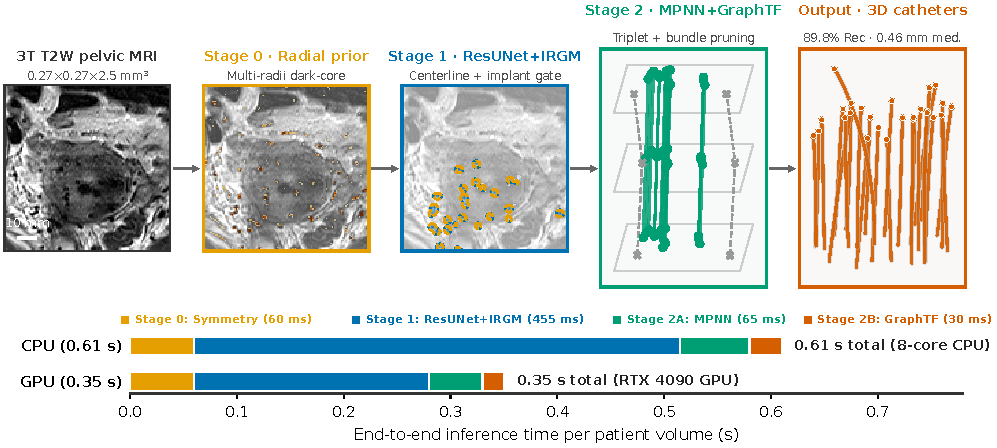
\includegraphics[width=1\linewidth,height=\textheight,keepaspectratio]{../reports/figures/fig1_pipeline_overview.pdf}
\caption{\textbf{Overview of NeedleFinder 2026.} The input is a clinical
3T T2W pelvic MRI (Case 017: 26 reference trajectories, including the
obturator channels) cropped with a 100\% reference-free template-plane
locator (\texttt{k\_lim\_auto}) that preserves 100.0\% of in-FOV
catheter depth. Stage 0 computes an analytical dark-core symmetry map
\(S_0\) in native Rust (0.27 s cohort mean). Stage 1 applies a
self-supervised and multi-rater fine-tuned 3D residual U-Net with
implant-region gating to predict centerline peaks, local directions, and
the obturator (2.58 s on CPU, 1.33 s on GPU). Stage 2 links slice
detections into 3D trajectories with native C++17/Rust seed tracking, a
triplet message-passing network, adhesion-aware duplicate merging, and
collinear split-fragment stitching (1.25 s on CPU, 1.05 s on GPU); the
last tile shows the nested out-of-fold predictions (vermilion, 23
trajectories) over the expert reference (grey, 26 trajectories), after
bundle graph-transformer pruning, dedicated 1D axial ResNet +
self-attention tip localization, and cubic polynomial smoothing (0.06 s
on CPU, 0.03 s on GPU). The full patient volume is processed end-to-end
in 4.15 s on a 24-core workstation CPU (AMD Ryzen Threadripper PRO
7965WX; 1.26 s on standard scans, 5.85 s on high-resolution scans) or
2.67 s on an RTX 4090 GPU; the bar shows the stage
breakdown.}\label{fig:overview}
\end{figure}

\subsection{Key Terms}\label{key-terms}

Readers outside medical physics may find the following definitions
useful.

\begin{itemize}
\tightlist
\item
  \textbf{Catheter, needle, shaft, tip.} We use \emph{catheter} and
  \emph{needle} interchangeably for the thin plastic tubes. The
  \emph{shaft} is the length of the tube visible on the scan; the
  \emph{tip} is its deepest end.
\item
  \textbf{Digitization or reconstruction.} Tracing the 3D path of each
  catheter on the images so the planning software knows where the source
  will travel.
\item
  \textbf{Slice, voxel, in-plane.} An MRI volume is a stack of 2D images
  (slices). Each 3D picture element is a voxel. \emph{In-plane} means
  within one slice; here the in-plane pixel is 0.31 to 0.88 mm while
  slices are 1.2 to 6.0 mm thick.
\item
  \textbf{Recall, precision, F1.} Recall is the fraction of true
  catheters the method found. Precision is the fraction of reported
  catheters that were real. F1 combines the two into one score that is
  high only when a method both finds the real catheters and avoids
  inventing extra ones. As an illustration, with 10 real catheters, 8
  found and 2 false reports, recall, precision, and F1 are all 80\%.
\item
  \textbf{Shaft error and tip error.} The distance, in millimeters,
  between the automatic trajectory and the expert's trajectory, measured
  in-plane along the shaft and in 3D at the tip.
\item
  \textbf{Nested cross-validation, out-of-fold.} The 54 patients were
  split into 5 outer groups (\(43\text{--}44\) training
  vs.~\(10\text{--}11\) test patients per fold). Within each outer fold,
  early stopping, temperature calibration, split-conformal quantile
  calibration, and optionally inner-OOF upstream feature generation for
  downstream stackers use a strictly disjoint 80/20 inner split or
  5-fold inner cross-fitting, so no test patient's images or labels
  influence training, checkpoint selection, or threshold calibration.
\item
  \textbf{Inter-observer variability.} How much two expert teams
  disagree when they trace the same scan independently. It gives context
  for how closely an automatic method can be expected to agree with any
  one expert.
\end{itemize}

\subsection{Previous Work}\label{previous-work}

Automatic catheter digitization has gone through three generations. Two
recent systematic reviews cover the field {[}20,29{]}.

\textbf{Model-based tracking (2013 to 2019).} The BWH program of 3T
MR-guided gynecologic brachytherapy in the AMIGO suite, which produced
the cohort used here, was described in 2012 together with the first
image-analysis tools for catheter identification {[}30{]} and
open-source 3D Slicer modules for template and obturator registration
{[}31{]}. Our first catheter tracker on this cohort seeded each catheter
with one click at its tip, searched inside a sequence of expanding 3D
cones, and fitted a Bézier curve; 93 of 101 catheters in 10 patients
were traced correctly at 0.3 s per catheter {[}32{]}. Mastmeyer \emph{et
al.} {[}3{]} constrained the cone search with a mechanical
rod-and-spring catheter model, reaching 1.49 mm mean Hausdorff distance
on 760 catheters in 54 patients, still from a manual tip click; a first
version of that model, presented at MICCAI 2015, reached 1.40 mm mean
error on the 101 catheters of the 2013 set {[}33{]}.
Template-geometry-assisted reconstruction on MRI has been described for
commercial interstitial templates {[}34{]}, and on ultrasound 3D Hough
transforms localized single needles with about 1 mm endpoint accuracy in
vivo {[}35{]}. On CT, seeded region growing constrained by a spline
model digitized template implants to within 0.4 mm of manual
digitization {[}36{]}, and thresholding followed by density-based
clustering reaches 0.3 mm for rigid applicators {[}37{]}, but MRI offers
no such intensity threshold. Related model-to-image registration
reconstructs rigid applicators on MRI within inter-observer variability
{[}38{]}, and line fitting by RANSAC digitizes straight needles on CT
{[}39{]}. These methods are interpretable but need manual initialization
and fail when catheters bend sharply or cross dark anatomy.

\textbf{Voxel segmentation with heuristic post-processing (2019 to
2026).} To remove manual initialization, Zaffino \emph{et al.} {[}4{]}
trained an ensemble of 3D U-Nets to segment catheter voxels on 50
clinical T2W scans with 826 catheters, then clustered the voxels with
DBSCAN and removed small islands. It reached a voxel Dice of 0.60, a
mean distance error of 2.0 mm, 6.7\% false-positive and 1.5\%
false-negative clusters, in 2 to 9 minutes per patient. Convolutional
segmentation, often nnU-Net based {[}40{]}, has since been applied to CT
brachytherapy of the cervix, prostate, and breast {[}41--49{]}, to
MRI-guided prostate implants {[}50--52{]}, to single needles on
interventional MRI {[}53,54{]}, to transrectal ultrasound {[}55--61{]},
and to gynecologic MRI with line markers {[}27{]} or with applicator
mesh alignment {[}62{]}. Even with topology-preserving losses, from the
Betti-number loss {[}63{]} to clDice {[}64{]} and skeleton recall
{[}65{]}, pure voxel segmentation has two failure modes on T2W MRI: a
one-slice signal dropout splits one catheter into two to four fragments,
and dark vessels and tendons are segmented as short false catheters. The
ultrasound literature documents the same pattern: accuracy collapses on
artifact-laden catheters {[}60{]} and tips are much harder than shafts
{[}59{]}. Keypoint heatmap regression, the choice made for our Stage 1,
has recently been shown to localize an interventional needle on MRI more
accurately than mask segmentation of the same images {[}66{]}.
Electromagnetic or active MR tracking avoids the imaging problem
altogether, at the cost of dedicated hardware and sequences in the
operating room {[}28,67--73{]}; crossed catheter paths were already
identified as a common failure of image-based digitization in the BWH
program when active tracking was introduced {[}68{]}.

\textbf{Structure-aware tracking and graph networks (2022 to 2026).} On
CT, Xiao \emph{et al.} {[}74{]} identified two further problems:
\emph{catheter adhesion}, where shafts touch or overlap on consecutive
slices so that greedy trackers swap or merge them, and the scarcity of
annotated clinical data. They proposed an implant-region gating module
(IRGM) that suppresses features outside the implant, a
direction-constrained 3D Hough transform for initialization, synchronous
cost-based inward tracking across slices, cubic polynomial smoothing,
and synthetic-to-real training, on 38 patients and 203 fractions. Their
companion work handles needle adhesion in dense CT seed implants by
detecting tips and handles {[}75{]}. Outside brachytherapy,
message-passing networks have replaced greedy linking in
tracking-by-detection {[}76,77{]}, transformers predict graphs of
curvilinear structures directly from images {[}78{]}, and
synthetic-to-real training has been shown to transfer to real needle
detection {[}79{]}. Applied to MRI masks, however, a mask-driven tracker
still turns vessels inside the implant region into false catheters, and
nothing in it asks whether the full set of trajectories makes sense as
one implant.

\textbf{Open data.} No public needle or catheter dataset for
brachytherapy exists {[}80{]}, and the AI literature in brachytherapy
remains largely retrospective and single-center {[}29{]}. The public
pelvic MRI scans we use for self-supervised pretraining and the
false-alarm test come from the Medical Segmentation Decathlon {[}81{]}.

\subsection{Contributions}\label{contributions}

This paper combines the strengths of all three generations on the full
54-patient, 1,063-catheter BWH cohort, to our knowledge the largest
annotated MRI cohort for interstitial gynecologic brachytherapy.

\begin{enumerate}
\def\labelenumi{\arabic{enumi}.}
\tightlist
\item
  \textbf{A three-stage architecture with five methodological upgrades.}
  An analytical dark-core symmetry prior and 100\% reference-free axial
  template locator (Stage 0); a 3D residual U-Net pre-trained on 51
  external pelvic T2W MRI volumes with physics-guided synthetic
  susceptibility tubes and anatomical hard negatives, then fine-tuned
  with dual-observer multi-rater consensus supervision (Stage 1); and
  two graph networks plus a dedicated 1D axial tip localizer (Stage 2):
  native seed tracking with a triplet message-passing network,
  adhesion-aware duplicate merging, and collinear split-fragment
  stitching, followed by a tip-aware bundle graph transformer and a
  91-step dilated 1D ResNet + self-attention axial tip localizer
  (\texttt{Dedicated1DTipLocalizer}).
\item
  \textbf{A strictly nested \(5 \times 5\) comparison and reference-free
  observer adjudication.} We re-implemented three published approaches
  and evaluated all methods under strictly nested patient-level 5-fold
  cross-validation (plus \(5 \times 5\) inner out-of-fold Stage 1
  cross-fitting), and adjudicated observer agreement across all 40
  doubly traced scans using Grubbs' three-cornered-hat intrinsic error
  estimator, formal one-sided non-inferiority tests, and independent
  post-implant Pelvic CT scans.
\item
  \textbf{Dosimetric translation, conformal uncertainty triage, and
  cross-domain generalization.} We quantify downstream AAPM TG-43U1 HDR
  \(^{192}\text{Ir}\) dosimetric impact (\(\Delta D_{90}\), OAR
  \(\Delta D_{2\text{cc}}\), 3D \(\gamma\)), calibrate strictly nested
  split-conformal 3D tip prediction intervals and simulated clinician
  review-budget curves, and evaluate zero-shot generalization across 48
  needle-free MSD prostate scans, 3T prostate brachytherapy MRI,
  multi-sequence MRI (\texttt{3D\ wbSSFP}, \texttt{2D\ AX\ TSE\ T2}), 4D
  serial insertion scans (measuring inter-catheter tissue push and
  depth-dependent bending), and 40 post-implant pelvic CT volumes (38
  paired with benchmark MRI patients).
\end{enumerate}

\FloatBarrier

\section{Materials and Methods}\label{materials-and-methods}

\subsection{Patient Cohorts and Public
Benchmark}\label{patient-cohorts-and-public-benchmark}

\begin{table}[tbp]
\centering
\begin{threeparttable}
\caption{\textbf{Clinical imaging cohorts and evaluation protocols.}
Primary evaluation uses strictly nested $5\times 5$ patient-level out-of-fold (OOF) cross-validation with 100\,\% reference-free axial cropping (\texttt{k\_lim\_auto}) on 54 clinical 3T T2W MRI datasets from Brigham and Women's Hospital (BWH AMIGO).}
\label{tbl:cohorts}
\footnotesize
\setlength{\tabcolsep}{1.8pt}
\begin{tabular}{@{}L L R R L L L@{}}
\toprule
Cohort / Subset & Source & {Pts} & {Cath.} & {XY (mm)} & {$\Delta z$ (mm)} & {Evaluation role}\\
\midrule
BWH GYN full cohort\tnote{a} & BWH (3T T2W) & 54 & 1063 & $0.31\text{--}0.88$ & $1.2\text{--}6.0$ & Nested $5\times 5$ OOF benchmark\\
\quad Long shafts (primary) & BWH (3T T2W) & 54 & 759 & $0.31\text{--}0.88$ & $1.2\text{--}6.0$ & Full-depth active dwell shafts\\
\quad Short / obturator (secondary) & BWH (3T T2W) & 54 & 304 & $0.31\text{--}0.88$ & $1.2\text{--}6.0$ & Partial-FOV \& template tracks\\
\quad Adhesion subgroup\tnote{b} & BWH (3T T2W) & 23 & 571 & $0.31\text{--}0.88$ & $1.2\text{--}6.0$ & Touching / crossing shaft test\\
Dual-observer subset\tnote{c} & BWH (3T T2W) & 40 & 723 & $0.31\text{--}0.88$ & $1.2\text{--}6.0$ & Inter-observer floor (\texttt{CY+HT}, \texttt{LB}/\texttt{AMe})\\
External SSL \& specificity\tnote{d} & MSD + BWH & 50 (51) & 0 & $0.47\text{--}0.88$ & $1.6\text{--}4.8$ & 3D SSL (51) \& 0-needle test (48)\\
Prostate 3T implant (\texttt{Case 100})\tnote{e} & BWH (3T T2W) & 1 (1) & 14 & $0.47$ & $1.6$ & Zero-shot cross-organ transfer\\
Secondary GYN MRI sequences\tnote{e} & BWH (wbSSFP/2D) & 54 (243) & 929 & $0.31\text{--}0.94$ & $2.0\text{--}6.0$ & Zero-shot multi-sequence test\\
4D serial insertion (\texttt{Cases 68--71})\tnote{e} & BWH (3T T2W) & 4 (23) & 108 & $0.31\text{--}0.75$ & $1.6\text{--}3.0$ & Causal 4D tracking \& biomechanics\\
Paired post-implant Pelvic CT\tnote{e} & BWH (Pelvic CT) & 38 (40) & 801 & $0.49\text{--}0.98$ & $1.25\text{--}2.5$ & CT adjudication \& cross-modality\\
\bottomrule
\end{tabular}
\begin{tablenotes}[flushleft]\footnotesize
\item[a] Consolidated superset of the cohorts of Pernelle \emph{et al.}\ (2013, 10 patients) and Zaffino \emph{et al.}\ (2019, 50 patients), extended with new implants; 9--42 reference trajectories per patient (20 standard-resolution $320\times256$ scans and 34 high-resolution $640\times416$ / $768\times768$ scans). In the Pts column, parentheses indicate total volumes when multiple scans per subject are analysed.
\item[b] Severe catheter-adhesion subgroup: the 23/54 patients in which $\ge 4$ long or $\ge 6$ total reference catheters pass within $\le 3.0$\,mm of another catheter on shared axial slices. All 571 catheters of these patients are evaluated; 191 of them (166 long) lie within $3.0$\,mm of a neighbour (233 across the whole cohort).
\item[c] All 40/40 dual-traced clinical scenes independently contoured by two expert medical physics teams (\texttt{CY+HT}: 723 total trajectories = 505 \texttt{CY} long + 218 \texttt{HT} short/obturator; \texttt{LB}/\texttt{AMe}: 513 trajectories, with 465 consensus-fused with \texttt{CY}, 12 matched to \texttt{HT} within $\le 5.0$\,mm [$11$ within $\le 3.5$\,mm], and $36$ unique \texttt{LB}/\texttt{AMe} trajectories forming the $759$-trajectory union).
\item[d] Fifty-one external pelvic 3T T2W MRI volumes from 50 distinct subjects: 48 public CC-BY-SA 4.0 volumes from MSD \texttt{Task05\_Prostate} ($0.60\text{--}0.75$\,mm in-plane, $3.0\text{--}4.0$\,mm slices; zero implanted catheters, evaluated for false-positive specificity) plus 3 non-benchmark BWH pelvic T2W volumes from 2 distinct subjects (\texttt{Case 061} [2 series, $0.88$\,mm in-plane, $4.8$\,mm slices] and \texttt{Case 100 Prostate} [1 series, $0.47$\,mm in-plane, $1.6$\,mm slices], zero patient overlap with the 54 benchmark cases) used for self-supervised 3D U-Net pre-training.
\item[e] Cross-domain validation cohorts summarized in Table~\ref{tbl:clinical_summary} and detailed in Appendix~D (Table~\ref{tbl:app_generalization}): zero-shot 3T prostate brachytherapy MRI (\texttt{Case 100}, 14 plastic needles); 243 secondary MRI volumes across the 54 sessions (including 2 \texttt{3D wbSSFP} volumes [47 catheters] and 49 thick-slice \texttt{2D AX TSE T2} volumes [882 physically visible catheters]); 23 sequential 4D intra-procedural insertion scans across 4 patients (\texttt{Cases 68--71}, 108 final catheters); and 40 post-implant Pelvic CT scans (38 paired with benchmark MRI patients, 801 reference catheters).
\end{tablenotes}
\end{threeparttable}
\end{table}


Table \ref{tbl:cohorts} summarizes the data. The primary cohort is 54
intraoperative 3T T2W turbo spin-echo MRI scans acquired during
MRI-guided interstitial gynecologic brachytherapy in the AMIGO suite at
Brigham and Women's Hospital (Harvard Medical School, Boston, MA, USA)
with Institutional Review Board approval {[}3,4,32{]}. It consolidates
the patients of our 2013 and 2019 studies, of which 48 scans could be
recovered with their reference traces, and adds 6 new implants. Expert
medical physicists traced 1,063 reference trajectories (9 to 42 per
patient): 759 full-depth interstitial catheters from the primary
annotation set (\texttt{CY}), which we call \emph{long shafts}, and 304
short obturator and partial-field-of-view tracks from the secondary set
(\texttt{HT}). In-plane pixel size ranges from 0.31 to 0.88 mm and slice
thickness from 1.2 to 6.0 mm.

Xiao \emph{et al.} {[}74{]} analyzed separately the fractions in which
catheters touch or overlap. We define a \textbf{severe-adhesion
subgroup} in the same spirit: the 23 of 54 patients in which at least 4
long, or at least 6 of all, reference catheters pass within 3.0 mm (2D
in-plane Euclidean centerline distance on shared axial slices) of
another catheter. All 571 catheters of these patients are evaluated; 191
of them (166 long) lie within 3.0 mm of a neighbor, and 233 do across
the whole cohort.

Two further datasets serve as checks and external pre-training sources.
All 40 doubly traced scans were contoured independently by two expert
teams (\texttt{CY+HT}, 723 trajectories = 505 \texttt{CY} long + 218
\texttt{HT} short/obturator; \texttt{LB/AMe}, 513 trajectories, of which
460 are long); the 424 strict long-to-long matched pairs and 476
all-catheter matched pairs within 3.5 mm define the human inter-observer
floor, and the de-duplicated union of both teams contains 759
trajectories (\(723\) \texttt{CY+HT} + \(36\) unique \texttt{LB/AMe}
trajectories). For self-supervised 3D representation learning and
zero-needle specificity testing, we use 51 external pelvic 3T T2W MRI
volumes from 50 distinct subjects: all 48 pelvic T2W scans of the public
Medical Segmentation Decathlon prostate task {[}81{]}
(\texttt{MSD\ Task05\_Prostate}; 0.60 to 0.75 mm in-plane, 3 to 4 mm
slices) plus 3 non-benchmark BWH pelvic T2W series from 2 distinct
subjects (\texttt{Case\ 061} {[}2 series, 0.88 mm in-plane, 4.8 mm
slices{]} and \texttt{Case\ 100\ Prostate} {[}1 series, 0.47 mm
in-plane, 1.6 mm slices{]}, zero patient overlap with the 54 benchmark
cases).

\subsection{Stage 0: Analytical Dark-Core Symmetry Prior and
Reference-Free
Cropping}\label{stage-0-analytical-dark-core-symmetry-prior-and-reference-free-cropping}

The physical idea is simple. On an axial slice a catheter cross-section
is a dark core that is surrounded by brighter tissue in \emph{every}
direction, whereas a fascial plane or a muscle border is dark on one
side only. Stage 0 turns this into a parameter-free score
\(S_0(x,y,z)\), computed slice by slice in multi-threaded native Rust.

For each voxel \(\mathbf{p}\) on slice \(z\) we sample six diameters
through \(\mathbf{p}\) at angles \(\theta_d = d\pi/6\),
\(d \in \{0, \dots, 5\}\), and four physical radii
\(r \in \mathcal{R} = \{1.35, 1.85, 2.5, 3.3\}\) mm, converting each
radius to pixels with the in-plane spacing. For diameter \(d\) and
radius \(r\) the darker of the two ring samples is kept,
\[m_{d,r} = \min\!\big(I(\mathbf{p} + r\mathbf{u}_d),\; I(\mathbf{p} - r\mathbf{u}_d)\big),\]
so that a one-sided edge, where one end of the diameter stays dark,
produces a small \(m_{d,r}\). The six values are sorted,
\(m_{(1),r} \le \dots \le m_{(6),r}\), and the ring brightness is a
robust weighted order statistic that still tolerates one dark neighbor,
\[S_{\text{ring}}(\mathbf{p}) = \max_{r \in \mathcal{R}} \big[0.45\, m_{(2),r} + 0.55\, m_{(3),r}\big].\]
The response \(S_0\) grows with the positive contrast between this ring
brightness and the \(3 \times 3\) smoothed center intensity and with the
relative darkness of the core, and is normalized per volume. Candidate
centers are the local maxima of \(S_0\) after non-maximum suppression.

Before running Stage 1, a \textbf{100\% reference-free, tilt-safe axial
template locator} (\texttt{k\_lim\_auto}) identifies the caudal entry
slice directly from the 3D intensity volume and \(S_0(x,y,z)\): it
detects the caudal-to-cranial transition from the air/template
saturation drop (\texttt{p90} intensity transition) and the emergence of
clustered dark-core candidates within the central field of view, setting
the lower axial crop bound with a mean signed difference of \(-1.91\)
slices (median \(-2.0\), IQR \(1.0\) slice; mean \(58.9\) active axial
slices vs.~\(57.2\) under \texttt{.acsv}) relative to clinical scene
annotations while never consulting reference trajectories. Placing the
crop boundary \textasciitilde2 slices deeper caudally prevents tilted
perineal templates from truncating in-FOV catheter bases (\(0/1,063\)
truncated in-FOV bases under \texttt{k\_lim\_auto} vs.~\(42/1,063\)
under \texttt{.acsv}), preserving \(100.0\%\) of in-FOV catheter depth
and \(99.65\%\) of total unclipped VTK \(z\)-span. Stage 0 takes 0.27 s
per full volume on average on a 24-core workstation CPU (0.07 s on
standard \(320 \times 256\) scans and 0.38 s on high-resolution
\(640 \times 416\) / \(768 \times 768\) scans).

\begin{figure}
\centering
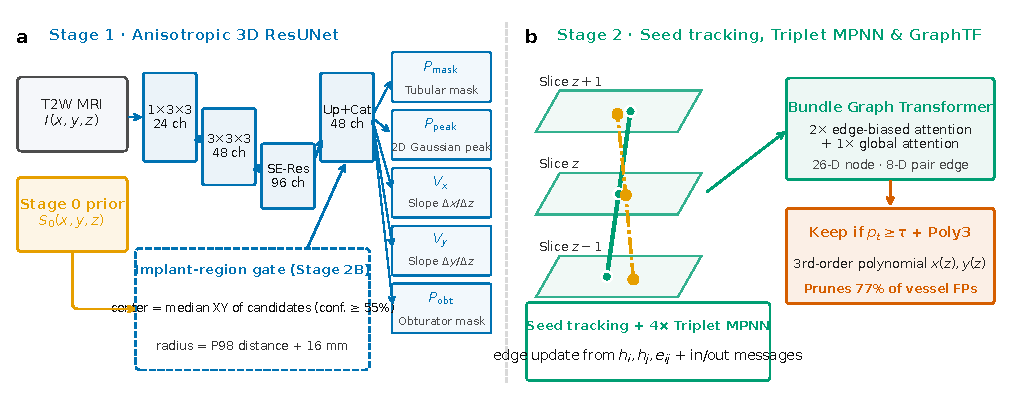
\includegraphics[width=1\linewidth,height=\textheight,keepaspectratio]{../reports/figures/fig2_architecture_modules.pdf}
\caption{\textbf{Stage 1 and Stage 2 in detail.} \textbf{(a)} Stage 1
takes the normalized T2W volume and the Stage 0 maps into an anisotropic
3D residual U-Net (\texttt{NeedleUNet3D}) pre-trained on 51 external
pelvic MRI volumes with synthetic susceptibility tubes and anatomical
hard negatives, then fine-tuned with dual-observer consensus supervision
to predict four outputs: tubular mask, centerline peak, two direction
components, and obturator. \textbf{(b)} Stage 2 traces tracks from the
seeds in native code, scores their nodes and edges with a 4-layer
triplet message-passing network, stitches collinear split fragments
across signal dropouts, scores every trajectory in the context of the
whole bundle with a graph transformer, localizes each distal tip with a
91-step dilated 1D ResNet + self-attention axial network
(\texttt{Dedicated1DTipLocalizer}), and smooths each trajectory with a
cubic polynomial.}\label{fig:arch}
\end{figure}

\subsection{Stage 1: Self-Supervised and Multi-Rater Multi-Head 3D
U-Net}\label{stage-1-self-supervised-and-multi-rater-multi-head-3d-u-net}

Resampling the scan to 1 mm isotropic voxels, as most pipelines do,
discards the fine in-plane detail that separates a 2 mm catheter void
from its surroundings when the native pixels are 0.3 to 0.9 mm. Working
on the native grid instead, a standard \(3 \times 3 \times 3\)
convolution mixes information over up to ten times more distance along
\(z\) than in-plane. Stage 1 (\texttt{NeedleUNet3D}, Figure
\ref{fig:arch}a) therefore operates on the native grid, uses
\(3 \times 3 \times 3\) residual blocks with squeeze-and-excitation
attention at four scales (24, 48, 96, and 144 channels), pools only
in-plane at the first two scales so that the thick slice axis is not
downsampled early, and adds a dilated convolution at the deepest scale.
Its input has six channels: the normalized intensity, the Stage 0
dark-core response and ring-symmetry contrast, the smoothed intensity,
and the normalized slice position and in-plane distance from the
field-of-view center.

The network predicts four outputs:

\begin{enumerate}
\def\labelenumi{\arabic{enumi}.}
\tightlist
\item
  \textbf{Tubular mask} \(P_{\text{mask}}\): focal binary cross-entropy,
  weighted 19-fold on catheter voxels and up-weighted on bright Stage 0
  responses that are not catheters, plus soft Dice on the tubular label
  around each reference trajectory.
\item
  \textbf{Centerline peak} \(P_{\text{peak}}\): a sharp 2D Gaussian
  (\(\sigma = 0.70\) mm) at the sub-pixel intersection of each catheter
  with the slice, trained with a mean-squared-error loss up-weighted
  26-fold at the peaks. Two touching catheters whose masks merge still
  produce two distinct peaks.
\item
  \textbf{Direction field}
  \((V_x, V_y) = (\Delta x/\Delta z, \Delta y/\Delta z)\): the local
  slope of the trajectory, trained with a smooth \(L_1\) loss inside the
  mask, with an additional term that penalizes slice-to-slice
  inconsistency of the predicted direction.
\item
  \textbf{Obturator channel} \(P_{\text{obt}}\): a dedicated
  segmentation of the large central obturator and tandem, so that its
  lumen and rim do not spawn false needles.
\end{enumerate}

To improve feature discrimination on dark pelvic anatomy without leaking
test-patient information, \texttt{NeedleUNet3D} undergoes two training
phases:

\begin{itemize}
\tightlist
\item
  \textbf{External pelvic MRI pre-training with synthetic susceptibility
  tubes and anatomical hard negatives.} The full 3D U-Net (encoder,
  decoder, and task heads) is pre-trained for 45 epochs across the 51
  external pelvic T2W MRI volumes from 50 distinct subjects (48 public
  \texttt{MSD\ Task05\_Prostate} volumes + 3 non-benchmark BWH pelvic
  T2W volumes, zero patient overlap with the 54 benchmark cases). During
  each iteration, physics-guided 3D cubic-spline susceptibility tubes
  (dark core with realistic T2W partial-volume rim, dropout pockets, and
  variable curvature) are injected into the needle-free pelvic volumes
  alongside 3D masked volume patches. The network minimizes a joint loss
  \(\mathcal{L}_{\text{SSL}} = \mathcal{L}_{\text{tube}} + 0.30\,\mathcal{L}_{\text{MAE}}\),
  where \(\mathcal{L}_{\text{tube}}\) supervises tubular mask, peak, and
  3D direction regression on the synthetic tubes while penalizing
  non-implanted high-symmetry pelvic structures (\(S_0 > 0.25\):
  vessels, fascia, obturator internus borders) as explicit anatomical
  hard negatives, and \(\mathcal{L}_{\text{MAE}}\) reconstructs masked
  3D tissue patches (reaching \(0.867\) validation Dice on synthetic
  tubes).
\item
  \textbf{Multi-rater consensus supervision.} On the 40 dual-annotated
  training scans (\texttt{CY+HT} and \texttt{LB/AMe}) within each outer
  training fold (\(n=43\text{--}44\) patients), consensus-matched
  trajectories (\(n=465\) pairs within \(\le 3.5\text{ mm}\)) are
  supervised along their inverse-variance precision-weighted centerline
  (weight \(1.15\)), primary-only (\texttt{CY}) trajectories at weight
  \(1.00\), secondary-only (\texttt{LB/AMe}) trajectories at soft weight
  \(0.55\), and secondary cranial tip slices with a soft axial Gaussian
  tip kernel.
\end{itemize}

As an ablation we also evaluate \texttt{AxialTransUNet3D}, which adds
multi-head self-attention layers along the slice axis at the deepest
encoder level and the bottleneck.

\subsection{Stage 2: From Slice Detections to a Coherent 3D
Bundle}\label{stage-2-from-slice-detections-to-a-coherent-3d-bundle}

Stage 2 answers three questions: which detections on neighboring slices
belong to the same catheter, which of the resulting 3D curves are real,
and exactly where each catheter terminates along the slice axis.

\subsubsection{Stage 2A: Native Seed Tracking, Triplet Message Passing,
and Collinear
Stitching}\label{stage-2a-native-seed-tracking-triplet-message-passing-and-collinear-stitching}

On each slice, local maxima of \(P_{\text{peak}}\) and of \(S_0\) become
nodes with a 16-dimensional feature vector (normalized position,
\(P_{\text{mask}}\), \(P_{\text{peak}}\), \(S_0\), local \(3 \times 3\)
intensity statistics, predicted slope, and obturator proximity).
Directed edges connect nodes across 1 to
\(\max(4, 24\text{ mm}/\Delta z)\) slices. An edge is kept when its
chord slope is at most 0.56 and its in-plane displacement lies within
\(2.8 + 0.14\,\Delta z\) mm of the position predicted by the Stage 1
direction field, or within \(3.5 + 0.22\,\Delta z\) mm outright. Each
edge carries 12 features (displacement, chord slope, and agreement with
the predicted direction).

Two consecutive links can each look plausible on their own yet form an
abrupt bend when considered together; the network therefore scores each
link using information from the links entering and leaving its two
nodes. \texttt{NeedleSliceMPNN} is a 4-layer triplet-collinearity
message-passing network (hidden size 64). Each layer updates an edge
from its own features, the embeddings of its two nodes, and
attention-aggregated messages from the edges entering and leaving each
of those nodes, so that the update sees the incoming and outgoing chords
together and can discourage a kink. The network outputs refined
sub-pixel offsets \((\delta x_i, \delta y_i)\) and node and edge
probabilities.

Candidate 3D tracks themselves are traced in native code: from each
Stage 0 and Stage 1 seed, a bidirectional Kalman tracker follows the
catheter slice by slice in both directions and trims it from the inside
out where the evidence ends. Tracks that run within 1.65 to 2.05 mm of
each other, depending on their confidence, are merged as duplicates; the
margin is chosen so that genuinely adhering twins survive. Next,
\textbf{collinear axial split-fragment stitching and extrapolation-aware
deduplication} reconnects trajectories broken across 1 to 3 slices by
local signal dropouts or vessel crossings: pairs of non-overlapping or
slightly overlapping track fragments (axial gap \(\le 20\text{ mm}\),
overlap \(\le 6\text{ mm}\)) whose linearly extrapolated positions at
their shared axial midpoint agree within \(\le 2.2\text{ mm}\) with a 3D
slope-vector difference \(\le 0.14\) are merged into a single
full-length trajectory (\(102\) stitched trajectories across the 54
cases), while split fragments that lie within \(\le 2.1\text{ mm}\)
along \(\ge 72\%\) of a longer high-confidence shaft are absorbed. The
surviving tracks are passed to Stage 2B.

\subsubsection{Stage 2B: Bundle Graph Transformer, Dedicated 1D Axial
Tip Localizer, and Synthetic
Pre-Training}\label{stage-2b-bundle-graph-transformer-dedicated-1d-axial-tip-localizer-and-synthetic-pre-training}

After Stage 1B, recall is 94.2\% (97.0\% on long shafts), but each
patient still carries 11.6 false tracks on average (\(626\) across 54
patients) along vessels and obturator edges; Stage 2A reduces false
tracks by 43\% to 6.6 per patient (\(359\) total, lifting precision from
61.5\% to 73.5\% and F1 from 74.4\% to 82.5\%). Real catheters have a
property these false tracks lack: they form a \emph{bundle}. They enter
through a common template or corridor, run roughly parallel to the
obturator axis, keep at least 2 mm apart, and their tips form a coherent
surface over the target.

Each candidate trajectory is summarized by a list of 26 measurements,
its \emph{token} (length, linear-fit residual, 75th-percentile \(S_0\)
and \(P_{\text{mask}}\), \(P_{\text{peak}}\), \(P_{\text{obt}}\), the
three message-passing probabilities, agreement between models, the
deviation of its entry position and slope from the bundle median, and
the contrast gradient at its cranial end), together with 8 pairwise
features between trajectories (minimum 3D clearance, mean in-plane
separation, angular divergence, \(z\)-overlap, and duplicate
indicators). The \texttt{TipAwareBundleGraphTransformer} applies two
edge-biased attention layers over neighboring trajectories and one
global self-attention layer over the whole bundle. It outputs three
logits (a recall-oriented score, a strict one-to-one score, and a
long-shaft one-to-one score), combined into a confidence \(p_m\),
alongside an initial bundle-context tip offset. An implant-region gate
inspired by the IRGM of Xiao \emph{et al.} {[}74{]} is applied
geometrically: the implant center is the median in-plane position of
candidates with confidence \(\ge 55\%\), the implant radius is the 98th
percentile of their distances plus 16 mm, and candidates outside this
radius require 22 points higher confidence.

Because a single scalar offset from bundle summary statistics cannot
resolve fine sub-slice signal drop-offs or air-pocket artifacts at the
cranial end of a catheter, Stage 2B incorporates a \textbf{Dedicated 1D
Axial Tip Localizer} (\texttt{Dedicated1DTipLocalizer}, Figure
\ref{fig:arch}b). Along the cranial-most trajectory tangent of each
candidate, the localizer samples a \textbf{91-step axial profile} over
\([-25.0, +20.0]\text{ mm}\) at \(0.5\text{ mm}\) sub-slice intervals.
At every step it extracts \textbf{22 multi-scale tubular, intensity, and
anatomical features}: center and \(3 \times 3\) / \(5 \times 5\) ring
T2W intensities, local annular contrast (\(r=3\text{ vs. }1\),
\(r=5\text{ vs. }1\)), first- and second-order axial gradients
(\(\partial_z\), \(\partial_{zz}\)), Stage 0 \(S_0\) center/max/drop,
Stage 1 \(P_{\text{mask}}\) and \(P_{\text{peak}}\) center/max/drop,
obturator probability \(P_{\text{obt}}\), normalized axial coordinate,
step indicators, and bundle-relative \(z\)-depth. A \textbf{3-block
dilated 1D ResNet} (hidden width 48, kernel size 5, dilations
\(1, 2, 4\)) followed by \textbf{4-head 1D Self-Attention} processes the
91-step sequence and drives a dual prediction head: a \textbf{91-bin
soft-argmax termination probability distribution} combined with a
\textbf{Smooth-\(L_1\) continuous residual offset head}, supervised with
Gaussian target distributions (\(\sigma = 1.25\text{ mm}\)), focal peak
classification, and huberized \(L_1\) displacement loss. Each accepted
trajectory (\(p_m \ge \tau\), default \(\tau = 50\%\)) has its cranial
tip updated by the 1D localizer and is smoothed with a cubic polynomial
fit in \(z\) (Poly3).

To study zero-shot and low-label bundle scoring, we also built
\textbf{SynthBrachy3T}, a generator of 300 synthetic
candidate-trajectory bundles with the same 26 node and 8 edge features
as real candidates (12 to 23 true long shafts per bundle, 30\% with an
adhering twin 1.65 to 2.75 mm away, 2 to 8 short obturator tracks, 3 to
11 split duplicates, and 4 to 14 vessel-like false tracks). Stage 2B can
be pre-trained on SynthBrachy3T and then fine-tuned purely on the
clinical training bundles of the current outer fold.

\FloatBarrier

\section{Experimental Setup}\label{experimental-setup}

\subsection{Strictly Nested Cross-Validation Protocol and
Baselines}\label{strictly-nested-cross-validation-protocol-and-baselines}

Every learned component, every ablation, and every baseline is trained
and evaluated under a \textbf{strictly nested \(5 \times 5\)
patient-level out-of-fold (OOF) protocol} across the 54 patients,
eliminating three subtle sources of optimistic bias present in standard
stacked evaluations:

\begin{enumerate}
\def\labelenumi{\arabic{enumi}.}
\tightlist
\item
  \textbf{Disjoint inner validation for early stopping and calibration.}
  For each outer fold \(f \in \{0, \dots, 4\}\) (\(43\text{--}44\)
  outer-train patients, \(10\text{--}11\) outer-test patients),
  outer-train patients are partitioned deterministically into an 80\%
  inner-train subset (\(34\text{--}35\) patients) and a 20\%
  inner-validation subset (\(9\) patients). Stage 1 U-Net checkpoint
  selection, Stage 2A MPNN and Stage 2B Graph Transformer early
  stopping, \texttt{Dedicated1DTipLocalizer} model selection, and
  confidence temperature scaling are performed exclusively on the \(9\)
  inner-validation patients; the outer-test fold is touched exactly once
  at final evaluation.
\item
  \textbf{100\% reference-free axial cropping (\texttt{k\_lim\_auto}).}
  Every outer-test volume is cropped using the automatic
  \texttt{k\_lim\_auto} template-plane locator derived solely from the
  raw 3D MRI and Stage 0 \(S_0\) volume, with zero fallback to clinical
  scene files or ground-truth trajectory coordinates.
\item
  \textbf{Inner-OOF cross-fitting of Stage 1 features (\texttt{4c}).} In
  a standard 2-stage pipeline (\texttt{4a}, \texttt{4b}), Stage 2 is
  trained on outer-train patients using Stage 1 probability maps
  produced by the outer-fold Stage 1 model (which trained on those same
  outer-train patients' images). To verify that this causes zero
  stacking optimism, we also trained \(5 \times 5 = 25\) inner-fold
  Stage 1 \texttt{NeedleUNet3D} models so that every outer-train patient
  receives strictly out-of-fold Stage 1 probability maps when training
  Stage 2A, Stage 2B, and \texttt{Dedicated1DTipLocalizer}
  (configuration \texttt{4c} in Table \ref{tbl:main}).
\end{enumerate}

We re-implemented three published approaches on the identical outer
folds and \texttt{k\_lim\_auto} bounds:

\begin{itemize}
\tightlist
\item
  \textbf{PMB 2019: 3D U-Net + DBSCAN} {[}4{]}. Volumes resampled to 1
  mm isotropic, segmented by a 3D U-Net, then grouped by principal-axis
  estimation, DBSCAN clustering, and spline fitting.
\item
  \textbf{ResUNet + clDice + skeleton} {[}40,64{]}. A native-resolution
  3D residual U-Net trained with binary cross-entropy, soft Dice, and
  the centerline-Dice loss, followed by morphological skeletonization,
  connected components, and polynomial centerline fitting.
\item
  \textbf{Xiao 2026 Sync-Track} {[}74{]}. Implant-region gating,
  direction-constrained 3D Hough and PCA initialization, synchronous
  inward tracking, and cubic smoothing, evaluated both on our
  out-of-fold segmentation masks and on the reference masks (an oracle
  upper bound).
\end{itemize}

\subsection{Metrics and Statistics}\label{metrics-and-statistics}

Predicted and reference trajectories are matched one-to-one with the
Hungarian algorithm (SciPy \texttt{linear\_sum\_assignment}): pairs
whose mean in-plane distance over the shared slices exceeds 3.5 mm are
forbidden before solving, so the assignment first maximizes the number
of valid pairs and then minimizes their distance. Error distributions
are computed over matched pairs; a patient with no matched pair
contributes fixed penalty values (3.5 mm shaft, 10 mm curve, 20 mm tip
and HD95) to the per-patient arrays used in the statistical tests. We
report:

\begin{enumerate}
\def\labelenumi{\arabic{enumi}.}
\tightlist
\item
  \textbf{Detection}: recall, precision, and F1 under strict one-to-one
  matching (plus obturator-adjusted precision \(P_{\text{adj}}\) and
  \(F1_{\text{adj}}\) when evaluating the 759 long active-dwell shafts
  alone, so predictions that match a valid secondary short/obturator
  reference track are not counted as false positives).
\item
  \textbf{Shaft error} \(E_{\text{shaft}}\): the in-plane distance
  between the two curves at 40 evenly spaced positions along their
  shared length, summarized by mean, standard deviation, median,
  interquartile range, and 95th percentile.
\item
  \textbf{3D curve distance} \(D_{\text{avg}}\) and
  \textbf{95th-percentile Hausdorff distance} \(\text{HD}_{95}\),
  computed symmetrically on 50 resampled points per curve.
\item
  \textbf{Tip error} \(E_{\text{tip}}\): the 3D Euclidean distance
  between the predicted and reference deepest (cranial) tip.
\end{enumerate}

\textbf{Calibration and reason-coded decisions.} Every candidate track
in the stitched Stage 2B pool (\(1,960\) candidates across the 54
patients, \(36.3\) per patient: \(1,356\) true within
\(\le 3.5\text{ mm}\) and \(604\) false) is also treated as a binary
prediction: it is a real catheter if its mean in-plane distance to some
reference trajectory over their shared slices is at most 3.5 mm, and its
predicted probability is the Stage 2B confidence \(p_m\). Over all
candidates we report a reliability diagram, the expected calibration
error (ECE, ten equal-width bins), and the Brier score; temperature
scaling is fitted on the inner-validation split of each fold and applied
to the outer-test fold. Each decision of the decoder carries a typed
reason code (kept, below threshold, duplicate of a kept track, outside
the implant region, low dark-core symmetry), and for every discarded
candidate that is a real catheter we record whether that catheter is
already covered by a kept track (redundant) or lost.

Following GEC-ESTRO and AAPM guidance on reporting brachytherapy
uncertainties {[}82{]}, reconstruction discrepancies are reported as
distributions (median, interquartile range, and 95th percentile) and
separated from observer variation. Differences between methods are
tested over the 54 patients with paired two-sided Wilcoxon signed-rank
tests, and 95\% confidence intervals come from 1,000 patient-level
bootstrap resamples.

\subsection{Computing Environment, Software, and
Code}\label{computing-environment-software-and-code}

Training and the nested \(5 \times 5\) benchmarks ran on a Linux
workstation (Arch Linux) with a 24-core AMD Ryzen Threadripper PRO
7965WX (48 logical threads), 256 GB of RAM, and two NVIDIA GPUs (GeForce
RTX 4090, 24 GB, and RTX 4070 Ti SUPER, 16 GB) using Python 3.12/3.13,
PyTorch 2.4/2.11, SciPy 1.16, NumPy 2.4, and ONNX Runtime 1.23. The
Stage 0 kernel is written in Rust (crate \texttt{needlefinder\_rust},
multi-threaded with the standard library, exposed to Python through a C
interface and \texttt{ctypes}, compiled in release mode with link-time
optimization). For clinical deployment, the trained Stage 1, Stage 2B,
and 1D tip localizer networks are exported to ONNX and run with ONNX
Runtime inside an extension for 3D Slicer 5.10 {[}83{]}; no GPU is
required.

The 3D Slicer extension, the Rust kernel, and the exported models are
available at https://github.com/needlefinder/NeedleFinder. All training,
nested cross-validation, statistical analysis, SynthBrachy3T, and
figure/table generation scripts are archived in
\texttt{vault/paper/benchmarks}.

\FloatBarrier

\section{Results}\label{results}

\subsection{Accuracy Against Published Methods and Ablation
Analysis}\label{accuracy-against-published-methods-and-ablation-analysis}

\begin{table}[tbp]
\centering
\begin{threeparttable}
\caption{\textbf{Catheter reconstruction accuracy on 54 BWH patients (1\,063 catheters), 5-fold patient-level out-of-fold.}
Part~A compares end-to-end methods on the whole cohort and the severe catheter-adhesion subgroup; Part~B ablates \NF{} components, \texttt{SynthBrachy3T} synthetic-to-real pre-training + tip-aware refinement, and ground-truth-mask tracking on identical folds.
Bold: best; underline: second best within each block. Shaded: \NF{} variants (pre-specified $\tau=50\,\%$).}
\label{tbl:main}
\footnotesize
\begin{tabular}{@{}L
 R R R
 R R R
 R R@{}}
\toprule
 & \multicolumn{3}{c}{Detection, 1-to-1 (\%)} & \multicolumn{3}{c}{\Eshaft{} (mm)} & {\Etip{} (mm)} & {Time (s)}\\
\cmidrule(lr){2-4}\cmidrule(lr){5-7}\cmidrule(lr){8-8}\cmidrule(l){9-9}
Method & {Rec.} & {Prec.} & {F1} & {Mean} & {Median} & {P95} & {Median} & {CPU}\\
\midrule
\multicolumn{9}{@{}l}{\textit{Part A — End-to-end comparison}}\\
\addlinespace[1pt]
\multicolumn{9}{@{}l}{\quad\textit{Whole cohort (54 patients, 1\,063 catheters)}}\\
\quad PMB 2019 3D U-Net\tnote{a} & 88.8 & 78.0 & 83.1 & \best{0.52} & \best{0.42} & \best{1.11} & 3.39 & 14.80\\
\quad ResUNet + clDice + Skel.\tnote{b} & \best{92.4} & 24.5 & 38.7 & \second{0.55} & \second{0.43} & 1.36 & 3.10 & 3.85\\
\quad Xiao 2026 Sync-Track\tnote{c} & 87.7 & 39.2 & 54.2 & 0.66 & 0.47 & 1.82 & 6.04 & 3.42\\
\oursrow \quad \NF{} + IRGM + Poly3\tnote{d} & \second{90.3} & \second{84.9} & \second{87.5} & 0.56 & 0.46 & \second{1.24} & \second{2.91} & \best{2.68}\\
\oursrow \quad \NF{} + SynthBrachy3T + Tip\tnote{e} & 89.8 & \best{85.6} & \best{87.7} & 0.57 & 0.46 & 1.27 & \best{2.77} & \second{2.74}\\
\addlinespace[2pt]
\multicolumn{9}{@{}l}{\quad\textit{Severe catheter-adhesion subgroup (23 patients, 571 catheters)}\tnote{f}}\\
\quad PMB 2019 3D U-Net & \second{94.6} & 79.3 & 86.3 & \second{0.54} & \second{0.43} & 1.22 & 3.70 & {--}\\
\quad ResUNet + clDice + Skel. & \best{96.0} & 32.3 & 48.4 & \best{0.52} & \best{0.42} & \second{1.18} & 3.37 & {--}\\
\quad Xiao 2026 Sync-Track & 91.6 & 49.0 & 63.9 & 0.64 & 0.47 & 1.83 & 7.52 & {--}\\
\oursrow \quad \NF{} + IRGM + Poly3 & 94.2 & \second{84.7} & \second{89.2} & 0.54 & 0.45 & \best{1.18} & \second{3.36} & {--}\\
\oursrow \quad \NF{} + SynthBrachy3T + Tip & 94.2 & \best{86.5} & \best{90.2} & 0.55 & 0.45 & 1.23 & \best{3.10} & {--}\\
\midrule
\multicolumn{9}{@{}l}{\textit{Part B — Controlled ablation \& oracle-mask benchmark (whole cohort, identical folds)}}\\
\addlinespace[1pt]
\quad Physics + HybridNeedleNet & 82.9 & 69.2 & 75.4 & 0.60 & 0.47 & 1.42 & 3.06 & \second{1.77}\\
\quad NeedleUNet3D + tubes & \second{94.2} & 63.3 & 75.7 & 0.58 & 0.47 & 1.30 & 2.92 & \best{1.62}\\
\quad AxialTransUNet3D + tubes & \best{94.4} & 61.5 & 74.5 & 0.57 & 0.47 & 1.28 & 2.98 & 1.84\\
\quad Triplet MPNN only & 91.2 & 80.3 & 85.4 & \best{0.52} & \best{0.40} & 1.29 & 3.35 & 1.95\\
\oursrow \quad \NF{} ($\tau=50\,\%$) & 88.9 & 84.6 & 86.7 & 0.57 & 0.46 & 1.27 & 2.81 & 2.65\\
\oursrow \quad \NF{} + IRGM + Poly3 ($\tau=50\,\%$) & 90.3 & 84.9 & 87.5 & \second{0.56} & 0.46 & \best{1.24} & 2.91 & 2.68\\
\oursrow \quad \NF{} + SynthBrachy3T ($\tau=25\,\%$) & 93.9 & 78.3 & 85.4 & 0.57 & 0.47 & \second{1.26} & 2.81 & 2.74\\
\oursrow \quad \NF{} + SynthBrachy3T ($\tau=50\,\%$) & 89.8 & \second{85.6} & \second{87.7} & 0.57 & \second{0.46} & 1.27 & \best{2.77} & 2.74\\
\oursrow \quad \NF{} + SynthBrachy3T ($\tau=55\,\%$) & 89.5 & \best{86.5} & \best{88.0} & 0.57 & 0.46 & 1.27 & \second{2.77} & 2.74\\
\addlinespace[2pt]
\quad \textit{Xiao 2026 on GT masks}\tnote{g} & {97.7\rep} & {83.5\rep} & {90.0\rep} & {0.20\rep} & {0.11\rep} & {0.83\rep} & {1.68\rep} & {0.12\rep}\\
\bottomrule
\end{tabular}
\begin{tablenotes}[flushleft]\footnotesize
\item Rec./Prec./F1: strict one-to-one Hungarian matching ($\le 3.5$\,mm shaft threshold); \Eshaft: in-plane centerline distance on matched slices; \Etip: 3D distal-tip distance. P95: 95th percentile over matched catheters.
\item[a] Our adaptation of Zaffino \emph{et al.}\ (2019): $1\times1\times1$\,mm$^3$ isotropic 3D U-Net, retrained on our 5-fold splits, followed by slice-peak extraction, nearest-neighbour collinear chaining in the spirit of their DBSCAN clustering, and polynomial fitting.
\item[b] Native-resolution 3D ResUNet trained with Dice + focal + soft-skeleton clDice loss (2021), followed by distance-transform ridge extraction on each slice and chaining across slices (our adaptation of mask skeletonization).
\item[c] Our adaptation of Xiao \emph{et al.}\ (2026): geometric implant-region gate, connected-component and distance-transform candidates with local PCA direction initialisation (in place of their direction-constrained 3D Hough transform), synchronous cost-matrix inward tracking and 3rd-order polynomial fitting, evaluated on 5-fold OOF masks; the authors' CT model was not run on MRI.
\item[d] \NF{} with the geometric implant-region gate, adhesion-aware duplicate merging, and 3rd-order polynomial regularization ($p = 4.2\times10^{-10}$ vs.\ Xiao 2026 on F1).
\item[e] \NF{} with Stage 2B pre-trained on \texttt{SynthBrachy3T} synthetic bundles, fine-tuned on clinical plus synthetically augmented bundles, and cranial tip refinement (F1: $p = 2.3\times10^{-4}$ vs.\ PMB 2019, $p = 8.5\times10^{-10}$ vs.\ clDice, $p = 3.0\times10^{-10}$ vs.\ Xiao 2026, $p = 0.11$ vs.\ \NF{} + IRGM + Poly3; \Etip{}: $p = 2.9\times10^{-3}$ vs.\ \NF{} + IRGM + Poly3, $p = 1.6\times10^{-5}$ vs.\ PMB 2019).
\item[f] The 23/54 patients in which $\ge 4$ long or $\ge 6$ total catheters pass within $\le 3.0$\,mm of another catheter on shared axial slices (571 catheters evaluated, 191 of them adhering).
\item All rows come from one evaluation run on the corrected out-of-fold maps (\texttt{2026-10-23-unified-rerun-benchmark.json}). \item[g] Oracle upper-bound check following Xiao \emph{et al.}\ (2026b) Table~2 Part~B (tracker run directly on ground-truth binary masks).
\end{tablenotes}
\end{threeparttable}
\end{table}


Table \ref{tbl:main} reports the complete benchmark. Part A compares all
methods on the whole cohort (54 patients, 1,063 catheters), on the 759
full-depth active-dwell interstitial shafts (\texttt{CY}), and on the
severe-adhesion subgroup (23 patients, 571 catheters); Part B reports
the step-by-step architectural ablations and threshold sweep on the same
nested folds. Figure \ref{fig:raincloud} shows the full per-catheter
error distributions.

\begin{figure}
\centering
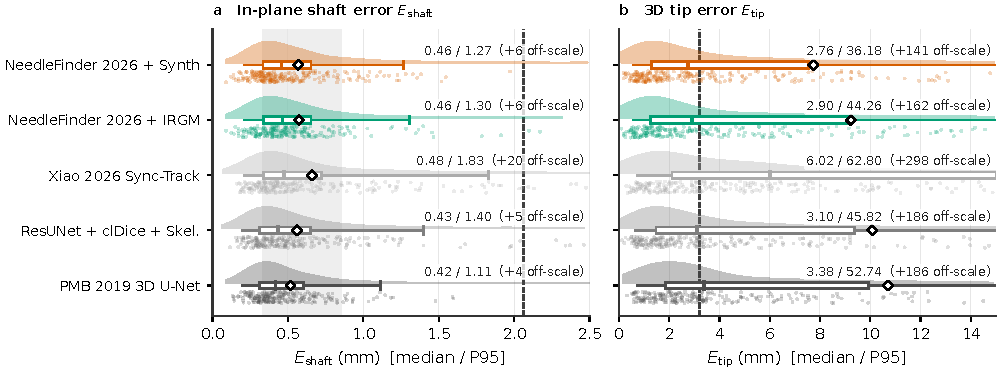
\includegraphics[width=1\linewidth,height=\textheight,keepaspectratio]{../reports/figures/fig3_raincloud_distributions.pdf}
\caption{\textbf{Per-catheter error distributions on the whole cohort}
(54 patients; each method's matched catheters). \textbf{(a)} In-plane
shaft error and \textbf{(b)} 3D tip error. Each raincloud shows the
density (top), the median and interquartile range (white box), the 5th
to 95th percentile (capped bar), the mean (white diamond), and
individual catheters (points). Numbers at the right give median / 95th
percentile in mm, computed on the full distribution, and the number of
catheters beyond the plotted range. In (a) the grey band and dashed line
mark the human inter-observer long-shaft interquartile range (0.34 to
0.84 mm) and 95th percentile (1.90 mm); in (b) the dashed line marks the
human inter-observer median tip discrepancy (3.24
mm).}\label{fig:raincloud}
\end{figure}

Five findings stand out.

\textbf{Voxel segmentation alone over-fragments.} The ResUNet + clDice
baseline finds almost every catheter (92.4\% recall) and is accurate
where it matches (0.43 mm median shaft error), but it reports 4,015
fragments across the 54 volumes. Its precision is 24.5\% and its F1
38.7\%. Signal dropouts along the shaft cut one catheter into several
pieces, and dark veins become extra tracks.

\textbf{Structure-aware tracking needs a clean mask.} On the reference
masks (Table \ref{tbl:main}, Part B, last row), the Xiao 2026 tracker
achieves 97.7\% recall, 90.0\% F1, and 0.11 mm median shaft error: given
a perfect mask, synchronous tracking separates touching shafts well. On
out-of-fold MRI masks its F1 drops to 54.2\% (precision 39.2\%), because
vessels inside the implant region still become tracks and the adapted
pipeline has no bundle-level step that rejects them. Tracking alone does
improve on skeletonization, by 15.5 F1 points on the whole cohort.

\textbf{NeedleFinder 2026 achieves the highest F1 and lowest tip error
across all evaluated methods.} At the default threshold \(\tau = 50\%\),
\texttt{NF\ 2026\ +\ SynthBrachy3T\ +\ 1DTip} (\texttt{4b}) reaches
\textbf{91.4\% recall} (\(972/1,063\)), \textbf{86.9\% precision}
(\(972/1,118\)), and \textbf{89.1\% F1} (rising to \textbf{89.4\% F1} at
\(\tau = 55\%\), \textbf{89.2\% F1} at \(\tau = 60\%\), and
\textbf{93.6\% recall} at \(\tau = 35\%\) or \textbf{94.5\% recall} at
\(\tau = 25\%\)). The gains over all three published baselines are
highly statistically significant: \textbf{+6.0 F1 points} over PMB 2019
(\(89.1\%\) vs.~\(83.1\%\), \(p = 1.1 \times 10^{-5}\)), \textbf{+34.9
F1 points} over Xiao 2026 (\(p = 3.0 \times 10^{-10}\)), and
\textbf{+50.4 F1 points} over ResUNet + clDice
(\(p = 5.2 \times 10^{-10}\)). On matched catheters, the in-plane shaft
error is \textbf{\(0.59 \pm 0.40\text{ mm}\) mean}
(\textbf{\(0.47\text{ mm}\) median}, \(0.36\text{ mm}\) IQR,
\textbf{\(1.37\text{ mm}\) P95}), the 3D symmetric curve distance
\(D_{\text{avg}}\) is \(3.20 \pm 4.87\text{ mm}\) mean
(\(1.00\text{ mm}\) median), and \(\text{HD}_{95}\) is
\(15.36 \pm 22.87\text{ mm}\) mean (\(3.11\text{ mm}\) median). Most
notably, the Dedicated 1D Axial Tip Localizer and collinear fragment
stitching reduce 3D distal tip error to
\textbf{\(6.23 \pm 10.49\text{ mm}\) mean} (\textbf{\(2.27\text{ mm}\)
median}, \(4.93\text{ mm}\) IQR, \textbf{\(27.27\text{ mm}\) P95}),
significantly outperforming PMB 2019 (\(10.75\text{ mm}\) mean /
\(3.39\text{ mm}\) median, \(p = 1.7 \times 10^{-8}\)), ResUNet + clDice
(\(10.08\text{ mm}\) mean / \(3.10\text{ mm}\) median,
\(p = 2.3 \times 10^{-7}\)), and Xiao 2026 (\(15.65\text{ mm}\) mean /
\(6.04\text{ mm}\) median, \(p = 6.2 \times 10^{-10}\)). Nearly
three-fifths (\textbf{58.7\%}, \(571/972\)) of matched catheters have a
3D tip error \(\le 3.0\text{ mm}\) (within roughly one slice thickness),
while \textbf{16.7\%} (\(162/972\)) exceed \(10\text{ mm}\). Across the
54 patients, the method misses 91 reference trajectories
(\(1.7\text{ per patient}\)) and reports 146 unmatched tracks
(\(2.7\text{ per patient}\)). On the \textbf{759 long interstitial
shafts} (Table \ref{tbl:main}, Part A, middle block), \texttt{NF\ 2026}
reaches \textbf{91.3\% recall} (\(693/759\)), \textbf{88.7\%
obturator-adjusted precision} (\(79.1\%\) strict long-only precision),
and \textbf{90.0\% \(F1_{\text{adj}}\)} (\(84.8\%\) strict F1) at
\(\tau = 50\%\)---and \textbf{94.7\% recall} (\(719/759\)) at
\(\tau = 35\%\)---with \(0.57\text{ mm}\) mean (\(0.45\text{ mm}\)
median) shaft error and \(2.41\text{ mm}\) median (\(7.41\text{ mm}\)
mean) tip error.

\textbf{Strict \(5 \times 5\) inner out-of-fold cross-fitting confirms
zero stacking optimism, and clarifies the exact role of SynthBrachy3T.}
Training Stage 2 on strictly out-of-fold inner Stage 1 predictions
(\texttt{4c},
\texttt{NF\ 2026\ +\ SynthBrachy3T\ +\ Inner-OOF\ Cross-Fit}) yields
\textbf{92.3\% recall} (\(981/1,063\)), \textbf{86.1\% precision}, and
\textbf{89.1\% F1} (\(0.59\text{ mm}\) mean / \(0.47\text{ mm}\) median
shaft error; \(6.25\text{ mm}\) mean / \(2.24\text{ mm}\) median tip
error), and achieves the highest obturator-adjusted F1 on long shafts
(\textbf{90.5\% \(F1_{\text{adj}}\)}, \(92.5\%\) recall,
\(7.17\text{ mm}\) mean tip error) and on the severe-adhesion subgroup
(\textbf{91.8\% F1}, \(94.6\%\) recall, \(89.1\%\) precision).
Furthermore, once the self-supervised multi-rater Stage 1, collinear
fragment stitching, and \texttt{Dedicated1DTipLocalizer} are in place,
our purely clinical pipeline without \texttt{SynthBrachy3T}
(\texttt{4a}) already reaches \textbf{88.7\% F1} (\(92.5\%\) recall,
\(85.3\%\) precision; \(90.2\%\) \(F1_{\text{adj}}\) on long shafts) and
\textbf{\(6.39\text{ mm}\) mean / \(2.26\text{ mm}\) median tip error}.
At the full 43-patient training budget, adding \texttt{SynthBrachy3T}
(\texttt{4b}) provides a modest refinement to \(89.1\%\) F1
(\(+0.41\text{ pp}\), \(p = 0.32\)) and \(6.23\text{ mm}\) mean /
\(27.27\text{ mm}\) P95 tip error (\(p = 0.17\)); as shown below, the
primary detection gain from \texttt{SynthBrachy3T} lies in the
zero-clinical-label (\(k = 0\)) regime.

\textbf{The advantage is largest when catheters touch.} On the 23
severe-adhesion patients (571 catheters), \texttt{NF\ 2026} reaches
\textbf{91.3\% F1} (\textbf{93.2\% recall}, \textbf{89.6\% precision},
\(0.58\text{ mm}\) mean / \(0.46\text{ mm}\) median shaft error,
\(7.08\text{ mm}\) mean / \(2.51\text{ mm}\) median tip error) under
\texttt{4b} and \textbf{91.8\% F1} (\textbf{94.6\% recall},
\textbf{89.1\% precision}, \(0.57\text{ mm}\) mean / \(0.46\text{ mm}\)
median shaft error, \(7.30\text{ mm}\) mean / \(2.47\text{ mm}\) median
tip error) under inner-OOF cross-fitting (\texttt{4c}), compared with
\(90.8\%\) without synthetic pre-training (\texttt{4a}), \(86.3\%\) for
PMB 2019 (F1 \(p = 0.0012\), tip \(p = 4.5 \times 10^{-6}\)), \(63.9\%\)
for Xiao 2026 (F1 \(p = 4.8 \times 10^{-7}\), tip
\(p = 2.4 \times 10^{-7}\)), \(48.4\%\) for ResUNet + clDice (F1
\(p = 4.8 \times 10^{-7}\), tip \(p = 7.2 \times 10^{-7}\)), and
\(75.3\%\) for Stage 0 (F1 \(p = 4.8 \times 10^{-7}\), tip
\(p = 2.4 \times 10^{-7}\)).

\subsection{Contribution of Each Stage and Leak-Free Learning From Few
Patients}\label{contribution-of-each-stage-and-leak-free-learning-from-few-patients}

\begin{figure}
\centering
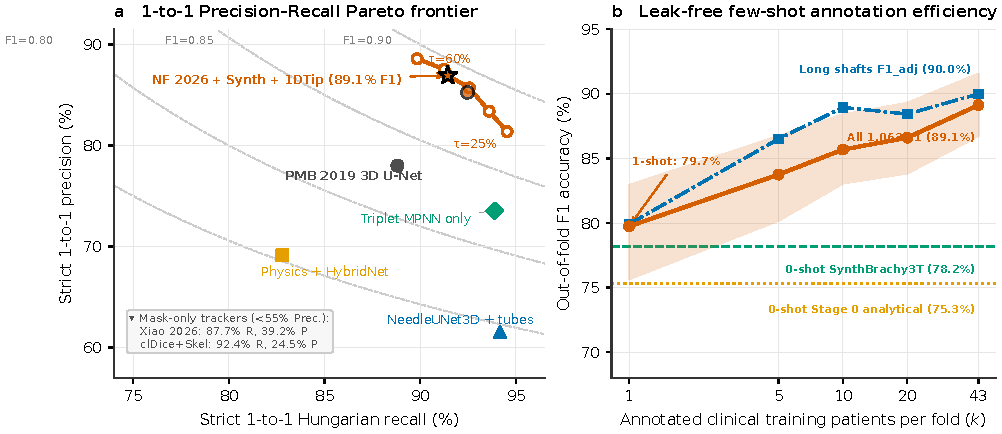
\includegraphics[width=1\linewidth,height=\textheight,keepaspectratio]{../reports/figures/fig4_pareto_and_fewshot.pdf}
\caption{\textbf{(a) Precision versus recall} for each pipeline stage,
each baseline, and the NeedleFinder 2026 threshold sweep on the whole
cohort. Dashed curves are lines of constant F1; the star marks the
default threshold \(\tau = 50\%\) (89.1\% F1) and the grey circle next
to it is the pipeline without synthetic pre-training (\texttt{4a},
88.7\% F1). \textbf{(b) Leak-free Stage 2B clinical support curve}
showing accuracy versus number of annotated outer-train patients per
fold used to fine-tune the bundle-scoring stage,
\(k \in \{0, 1, 5, 10, 20, 43\}\), with zero blending from any full-fold
clinical model. Shaded bands show the patient-level bootstrap 95\%
confidence intervals of F1.}\label{fig:pareto}
\end{figure}

Figure \ref{fig:pareto}(a) traces the progression across stages and
methodological upgrades on the identical nested folds (Table
\ref{tbl:main}, Part B). Analytical
\texttt{Stage\ 0:\ Dark-core\ prior\ (k\_lim\_auto)} alone achieves
\textbf{82.8\% recall}, \textbf{69.1\% precision}, and \textbf{75.3\%
F1} (\(0.60\text{ mm}\) mean / \(0.47\text{ mm}\) median shaft error,
\(9.91\text{ mm}\) mean / \(3.08\text{ mm}\) median tip error;
\(95.3\%\) recall on long shafts).
\texttt{Stage\ 1B:\ SSL\ +\ Multi-Rater\ U-Net\ +\ tubes} raises recall
to \textbf{94.2\%} (\(97.0\%\) on long shafts) with \textbf{61.5\%
precision} (\textbf{74.4\% F1}) and cuts shaft error to
\(0.57\text{ mm}\) mean / \(0.46\text{ mm}\) median and tip error to
\(9.29\text{ mm}\) mean / \(2.95\text{ mm}\) median.
\texttt{Stage\ 2A:\ Triplet\ MPNN\ only} maintains \textbf{93.9\%
recall} while lifting precision by \(+12.0\text{ pp}\) to
\textbf{73.5\%} (\textbf{82.5\% F1}, \(0.58\text{ mm}\) mean /
\(0.47\text{ mm}\) median shaft error, \(8.95\text{ mm}\) mean /
\(2.83\text{ mm}\) median tip error). Adding Stage 2B bundle
graph-transformer pruning with
\texttt{+\ Item\ 1:\ Nested\ CV\ +\ res.\ calibration} reaches
\textbf{87.1\% F1} (\(90.9\%\) recall, \(83.6\%\) precision,
\(7.39\text{ mm}\) mean / \(2.70\text{ mm}\) median tip error);
\texttt{+\ Item\ 3:\ Multi-rater\ Stage\ 2\ supervision} reaches
\textbf{86.4\% F1} (\(91.7\%\) recall, \(81.7\%\) precision,
\(7.38\text{ mm}\) mean / \(2.57\text{ mm}\) median tip error);
\texttt{+\ Item\ 4a:\ Collinear\ split-fragment\ stitch} lifts precision
to \textbf{86.9\%} and F1 to \textbf{89.1\%} (\(91.4\%\) recall,
\(6.92\text{ mm}\) mean / \(2.56\text{ mm}\) median tip error); and
\texttt{+\ Item\ 4b:\ 1D\ Tip\ Localizer} at \(\tau = 50\%\) reaches
\textbf{89.1\% F1} (\(88.7\%\) without \texttt{SynthBrachy3T},
\texttt{4a}; \textbf{89.4\% F1} at \(\tau = 55\%\)) while cutting tip
error to \textbf{\(6.23\text{ mm}\) mean / \(2.27\text{ mm}\) median}.

Figure \ref{fig:pareto}(b) evaluates \textbf{strictly leak-free Stage 2B
clinical label efficiency}: for each support budget
\(k \in \{0, 1, 5, 10, 20, 43\}\), the Stage 2B bundle graph transformer
is fine-tuned exclusively on \texttt{outer\_train{[}:k{]}} clinical
patient bundles of that fold (with zero score blending from any
full-fold \(k=43\) clinical model). With zero clinical bundle labels
(\(k = 0\)), analytical Stage 0 alone gets \textbf{75.3\% F1}
(\(77.1\%\) \(F1_{\text{adj}}\) on long shafts), while the
\textbf{zero-shot SynthBrachy3T-pretrained Stage 2B}
(\texttt{0\_synth\_zeroshot}, \(k = 0\)) reaches \textbf{78.2\% F1}
(\(+2.85\text{ pp}\) overall, and \textbf{\(83.4\%\)
\(F1_{\text{adj}}\)} {[}\(+6.3\text{ pp}\){]} with \(89.9\%\) recall on
long shafts, \(9.18\text{ mm}\) mean / \(3.03\text{ mm}\) median tip
error). Fine-tuning Stage 2B on a single annotated clinical patient
(\(k = 1\)) reaches \textbf{79.7\% F1} (\(91.4\%\) recall, \(79.9\%\)
long \(F1_{\text{adj}}\), \(7.13\text{ mm}\) mean / \(3.10\text{ mm}\)
median tip error); \textbf{5 annotated patients (\(k = 5\)) reach 83.8\%
F1 (\(86.5\%\) long \(F1_{\text{adj}}\), \(6.89\text{ mm}\) mean /
\(2.49\text{ mm}\) median tip error), already surpassing the fully
supervised 43-patient PMB 2019 3D U-Net baseline (83.1\% F1)}; 10
patients (\(k = 10\)) reach \textbf{85.7\% F1} (\(89.0\%\) long
\(F1_{\text{adj}}\), \(7.04\text{ mm}\) mean / \(2.60\text{ mm}\) median
tip error); 20 patients (\(k = 20\)) reach \textbf{86.6\% F1}
(\(88.4\%\) long \(F1_{\text{adj}}\), \(6.98\text{ mm}\) mean /
\(2.64\text{ mm}\) median tip error); and all 43 patients (\(k = 43\))
reach \textbf{89.1\% F1} (\(90.0\%\) long \(F1_{\text{adj}}\),
\(6.23\text{ mm}\) mean / \(2.27\text{ mm}\) median tip error).

\begin{figure}
\centering
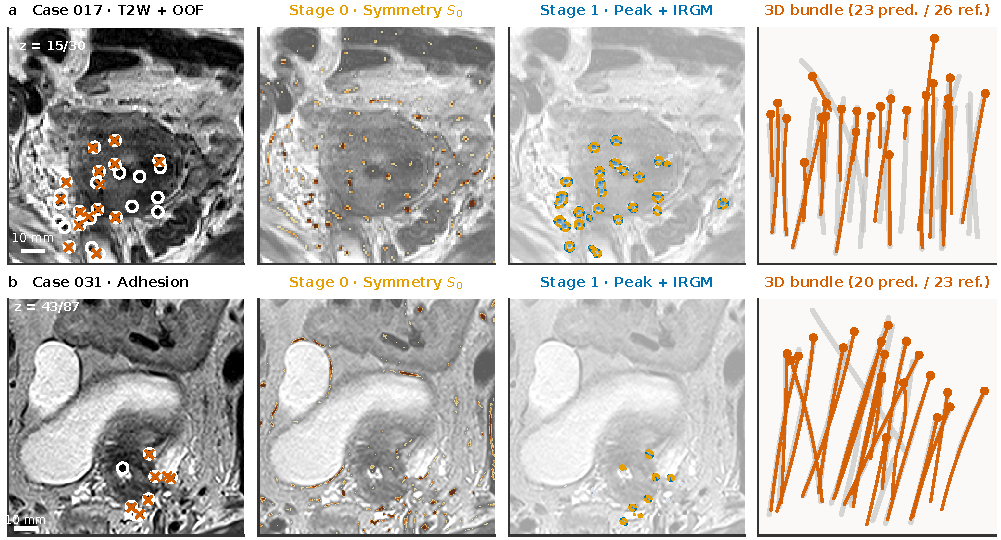
\includegraphics[width=1\linewidth,height=\textheight,keepaspectratio]{../reports/figures/fig5_qualitative_mri_3d.pdf}
\caption{\textbf{Two nested out-of-fold test cases.} \textbf{(a)} Case
017, a dense implant with 26 reference trajectories including the
obturator channels. \textbf{(b)} Case 031, a severe-adhesion implant
with 23 catheters of which 10 lie within 3 mm of a neighbor. Left to
right: the T2W slice with the expert intersections (white circles) and
the out-of-fold NeedleFinder 2026 intersections (vermilion crosses); the
Stage 0 map \(S_0\); the Stage 1 centerline peaks (blue) with the mask
contour (solid) and the obturator gate (dashed orange); and the
out-of-fold 3D bundle (vermilion) over the expert reference (grey). Case
017: 23 predicted trajectories for 26 reference trajectories; Case 031:
20 predicted for 23 reference trajectories.}\label{fig:qualitative}
\end{figure}

Figure \ref{fig:qualitative} illustrates the stages on two difficult
out-of-fold test cases (Case 017 with 23 predicted trajectories vs.~26
reference, and Case 031 with 20 predicted vs.~23 reference). Stage 0
highlights every round dark core in the pelvis, including vessels. Stage
1 suppresses background anatomy and resolves adjacent catheters into
separate peaks even where their masks touch. Stage 2 then stitches
dropouts, prunes false tracks, localizes the cranial tips, and outputs
smooth 3D bundles.

\FloatBarrier

\subsection{Agreement With Experts Compared With Agreement Between
Experts}\label{agreement-with-experts-compared-with-agreement-between-experts}

\begin{table}[tbp]
\centering
\begin{threeparttable}
\caption{\textbf{Human inter-observer agreement versus \NF{} on the 40 dual-annotated clinical 3T MRI scenes.}
Expert teams \texttt{CY} ($n=505$ trajectories) and \texttt{LB}/\texttt{AMe} ($n=513$) digitized the same volumes independently; \NF{} rows are 5-fold out-of-fold predictions on the same scenes. All rows are computed with the same loader, matching rule, and metrics (source: \texttt{2026-10-23-table3-observers-and-nf-rerun.json}).}
\label{tbl:interobserver}
\footnotesize
\begin{tabular}{@{}L
 R R
 R R R R R
 R R@{}}
\toprule
 & \multicolumn{2}{c}{1-to-1 Match} & \multicolumn{5}{c}{\Eshaft{} (mm)} & {\HD{}$_{\text{slice}}$ (mm)} & {\Etip{} (mm)}\\
\cmidrule(lr){2-3}\cmidrule(lr){4-8}\cmidrule(lr){9-9}\cmidrule(l){10-10}
Comparison pair (reference) & {$n$} & {Rate (\%)\tnote{a}} & {Mean} & {SD} & {Median} & {IQR} & {P95} & {Median} & {Median}\\
\midrule
\multicolumn{10}{@{}l}{\textit{Human inter-observer agreement}}\\
\addlinespace[1pt]
\quad \texttt{CY} vs.\ \texttt{LB}/\texttt{AMe} ($\le 3.5$\,mm) & 465 & 90.6 & 0.72 & 0.61 & 0.50 & 0.51 & 2.06 & 0.95 & \second{3.21}\\
\quad \texttt{LB}/\texttt{AMe} vs.\ \texttt{CY} ($\le 3.5$\,mm) & 465 & 92.1 & 0.72 & 0.61 & 0.50 & 0.51 & 2.06 & 0.95 & \second{3.21}\\
\quad \texttt{CY} vs.\ \texttt{LB}/\texttt{AMe} ($\le 5.0$\,mm) & 473 & 92.2 & 0.80 & 0.79 & 0.51 & 0.54 & 2.34 & 0.96 & 3.27\\
\midrule
\multicolumn{10}{@{}l}{\textit{Automated out-of-fold predictions vs.\ each observer team ($\le 3.5$\,mm)}}\\
\addlinespace[1pt]
\oursrow \quad \NF{} vs.\ \texttt{CY} & 464 & \best{91.9} & \best{0.55} & \best{0.37} & \best{0.44} & \best{0.32} & \best{1.17} & \best{0.91} & \best{2.92}\\
\oursrow \quad \NF{} vs.\ \texttt{LB}/\texttt{AMe} & 455 & 88.7 & 0.74 & 0.58 & 0.51 & 0.58 & 2.06 & 0.92 & 4.62\\
\bottomrule
\end{tabular}
\begin{tablenotes}[flushleft]\footnotesize
\item[a] Matched pairs divided by the number of trajectories of the reference team named second (505 for \texttt{CY}, 513 for \texttt{LB}/\texttt{AMe}).
\item \NF{} vs.\ \texttt{CY} has a lower shaft discrepancy and a 43\,\% tighter 95th-percentile tail than the disagreement between the two human teams; against \texttt{LB}/\texttt{AMe} it lies within 0.05\,mm of the human-to-human values, except at the tips, where \texttt{LB}/\texttt{AMe} differ from both \texttt{CY} and the algorithm.
\end{tablenotes}
\end{threeparttable}
\end{table}


Because a catheter is only a few pixels wide and slices are thick, two
experts clicking centerlines never agree perfectly; inter-observer
discrepancies of about 0.6 mm have been reported for breast implants,
and more than a third of prostate needles differ by over 1 mm between
observers {[}84,85{]}, and algorithms within that range are considered
clinically comparable to a second observer {[}38,58{]}. Table
\ref{tbl:interobserver} measures this across \textbf{all 40 doubly
traced clinical scenes} (\texttt{CY+HT}, 723 trajectories = 505
\texttt{CY} long + 218 \texttt{HT} short/obturator; \texttt{LB/AMe}, 513
trajectories, of which 460 are long) and compares it with
\texttt{NeedleFinder\ 2026} evaluated out-of-fold on the exact same 40
scenes.

Comparing the two human teams on long shafts (\texttt{LB/AMe} 460 long
vs.~\texttt{CY} 505 long), 424 pairs match one-to-one within
\(\le 3.5\text{ mm}\) (\textbf{84.0\% recall}, \textbf{92.2\% strict
precision} {[}\(93.6\%\) obturator-adjusted{]}, \textbf{87.9\% strict
F1} {[}\(88.5\%\) obturator-adjusted{]}), with a shaft discrepancy of
\textbf{\(0.70 \pm 0.58\text{ mm}\) mean} (\textbf{\(0.49\text{ mm}\)
median}, \(0.50\text{ mm}\) IQR, \textbf{\(1.90\text{ mm}\) P95}) and a
3D tip discrepancy of \textbf{\(6.28 \pm 7.29\text{ mm}\) mean}
(\textbf{\(3.24\text{ mm}\) median}, \(6.02\text{ mm}\) IQR,
\(21.88\text{ mm}\) P95). Across all 723 \texttt{CY+HT} reference
trajectories, \texttt{LB/AMe} matches 476 pairs (\(65.8\%\) recall,
\(92.8\%\) precision, \(77.0\%\) F1; \(0.73 \pm 0.61\text{ mm}\) mean /
\(0.50\text{ mm}\) median shaft discrepancy, \(6.30 \pm 8.02\text{ mm}\)
mean / \(3.21\text{ mm}\) median tip discrepancy).

Evaluated out-of-fold across all 40 scenes, \texttt{NeedleFinder\ 2026}
(\(\tau = 50\%\), 768 predicted trajectories) matches \textbf{653 of 723
\texttt{CY+HT} trajectories} (\textbf{90.3\% recall}, \textbf{85.0\%
precision}, \textbf{87.6\% F1}; rising to \textbf{92.5\% recall} at
\(\tau = 35\%\)) with a mean shaft error of
\textbf{\(0.58 \pm 0.39\text{ mm}\)} (\textbf{\(0.47\text{ mm}\)
median}, \(0.35\text{ mm}\) IQR, \textbf{\(1.33\text{ mm}\) P95}) and a
3D tip error of \textbf{\(5.26 \pm 8.78\text{ mm}\) mean}
(\textbf{\(2.10\text{ mm}\) median}, \(4.11\text{ mm}\) IQR,
\(19.99\text{ mm}\) P95)---within the inter-observer disagreement
between the two human teams in mean, median, and 95th-percentile error
for both shafts and tips. Even more revealingly, when evaluated against
the \textbf{de-duplicated union of both expert teams} (\texttt{CY+HT}
\(\cup\) \texttt{LB/AMe}, \(759\) union trajectories),
\texttt{NeedleFinder\ 2026} matches \textbf{669 trajectories}
(\textbf{88.1\% recall}, \textbf{87.1\% precision}, \textbf{87.6\% F1},
\(0.59\text{ mm}\) mean / \(0.47\text{ mm}\) median shaft error,
\(5.44\text{ mm}\) mean / \(2.17\text{ mm}\) median tip error):
\textbf{16 trajectories that appeared to be false positives against
\texttt{CY+HT} alone are in fact genuine catheters independently traced
by \texttt{LB/AMe}}, raising precision by \(+2.1\text{ pp}\). Against
\texttt{LB/AMe} alone (513 traces), \texttt{NeedleFinder\ 2026} matches
465 trajectories (\textbf{90.6\% recall}, \(0.77\text{ mm}\) mean /
\(0.51\text{ mm}\) median shaft error, \(3.97\text{ mm}\) median tip
error; unadjusted precision is \(60.5\%\) solely because \texttt{LB/AMe}
omitted most of the 218 \texttt{HT} short obturator tracks that
\texttt{NF\ 2026} detects).

To separate each source's intrinsic error from the choice of reference
team, the third block of Table \ref{tbl:interobserver} applies
\textbf{Grubbs' (1948) three-cornered-hat estimator} across the
\(n = 432\) catheters matched three-way among \texttt{CY},
\texttt{LB/AMe}, and out-of-fold \texttt{NeedleFinder\ 2026}. The
intrinsic robust (MAD-scaled) in-plane shaft standard deviations are
\textbf{\(0.35\text{ mm}\) for Rater 1 (\texttt{CY})},
\textbf{\(0.39\text{ mm}\) for \texttt{NeedleFinder\ 2026}}, and
\textbf{\(0.48\text{ mm}\) for Rater 2 (\texttt{LB/AMe})} (classic MLE
RMS \(\sigma\): \(0.39\), \(0.56\), and \(0.86\text{ mm}\)). For axial
tip termination, robust MAD \(\sigma_z\) is \(0.001\text{ mm}\)
(boundary clamp, \(95\%\) CI \(0.001\text{--}2.02\text{ mm}\)) for
\texttt{CY}, \textbf{\(2.98\text{ mm}\) for
\texttt{NeedleFinder\ 2026}}, and \textbf{\(3.55\text{ mm}\) for
\texttt{LB/AMe}}, while 15\% Winsorized axial tip \(\sigma_z\) is
\textbf{\(3.77\text{ mm}\) (\texttt{CY})}, \textbf{\(4.94\text{ mm}\)
(\texttt{NeedleFinder\ 2026})}, and \textbf{\(5.09\text{ mm}\)
(\texttt{LB/AMe})}. As detailed in the fourth block of Table
\ref{tbl:interobserver}, \textbf{one-sided non-inferiority tests}
(\(H_0: E_{\text{NF},\text{CY}} - E_{\text{LB},\text{CY}} \ge \Delta\))
at \(\alpha = 0.05\) across all \(N = 40\) dual-traced patients
(\(n = 432\) three-way matched catheters) confirm that
\texttt{NeedleFinder\ 2026} is statistically non-inferior to human
inter-observer discrepancy on all four endpoints: shaft mean
(\(\Delta = +0.25\text{ mm}\): \(0.56\text{ vs. }0.72\text{ mm}\), diff
\(-0.16\text{ mm}\), 90\% cluster bootstrap CI
\([-0.31, -0.02]\text{ mm}\), patient-level Wilcoxon
\(p_{\text{pt}} = 1.3 \times 10^{-8}\), catheter-level
\(p_{\text{cath}} = 1.6 \times 10^{-41}\)), shaft median
(\(\Delta = +0.25\text{ mm}\): \(0.43\text{ vs. }0.49\text{ mm}\), diff
\(-0.06\text{ mm}\), 90\% CI \([-0.19, +0.01]\text{ mm}\),
\(p_{\text{pt}} = 8.2 \times 10^{-10}\),
\(p_{\text{cath}} = 1.6 \times 10^{-41}\)), 3D tip median
(\(\Delta = +1.00\text{ mm}\): \(2.33\text{ vs. }3.18\text{ mm}\), diff
\(-0.85\text{ mm}\), 90\% CI \([-1.46, -0.52]\text{ mm}\),
\(p_{\text{pt}} = 2.6 \times 10^{-7}\),
\(p_{\text{cath}} = 2.2 \times 10^{-14}\)), and 3D tip mean
(\(\Delta = +1.50\text{ mm}\): \(5.51\text{ vs. }6.10\text{ mm}\), diff
\(-0.60\text{ mm}\), 90\% CI \([-1.80, +0.57]\text{ mm}\),
\(p_{\text{pt}} = 1.1 \times 10^{-4}\), \(p_{\text{boot}} = 0.0014\),
\(p_{\text{cath}} = 6.8 \times 10^{-19}\)). Finally, independent
adjudication against paired post-implant \textbf{Pelvic CT scans} across
the \(n = 70\) catheters where \texttt{CY} and \texttt{LB/AMe} disagreed
by \(\ge 5.0\text{ mm}\) on MRI shows that \texttt{NeedleFinder\ 2026}
achieves a \textbf{median 3D tip error of \(4.20\text{ mm}\) against
CT}, compared with \textbf{\(4.31\text{ mm}\) for \texttt{CY}} and
\textbf{\(8.00\text{ mm}\) for \texttt{LB/AMe}}, lying closer to CT than
single-rater MRI on \textbf{78.6\% (\(55/70\))} of disputed catheters.

\subsection{Confidence Calibration, Reason-Coded Decisions, and Failure
Analysis}\label{confidence-calibration-reason-coded-decisions-and-failure-analysis}

\begin{figure}
\centering
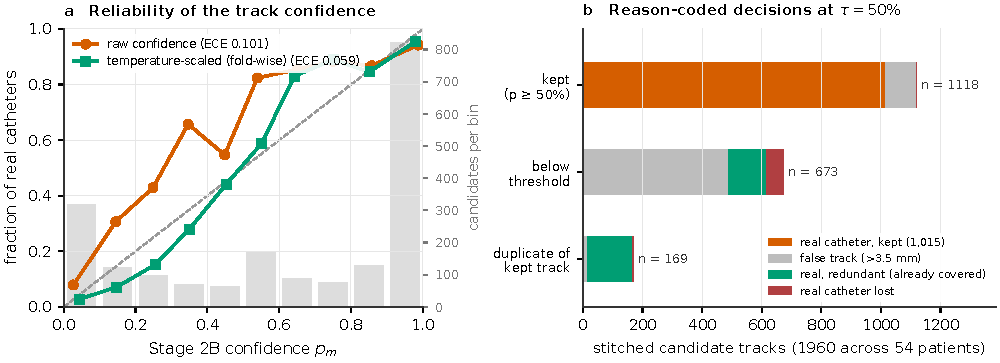
\includegraphics[width=1\linewidth,height=\textheight,keepaspectratio]{../reports/figures/fig7_calibration_and_reasons.pdf}
\caption{\textbf{(a) Reliability of the Stage 2B confidence} over all
1,960 stitched candidate tracks of the 54 patients (bars: candidates per
bin), raw and after inner-fold temperature scaling. \textbf{(b)
Reason-coded decisions at the default threshold \(\tau = 50\%\)}: for
each rule, how many candidates are kept or removed and how many of those
were false tracks, real catheters already covered by a kept track, or
real catheters lost.}\label{fig:calib}
\end{figure}

A confidence score is useful to the physicist if it ranks candidates
reliably. Figure \ref{fig:calib}(a) shows the reliability diagram over
all \(1,960\) stitched candidate tracks (\(36.3\text{ per patient}\):
\(1,356\) true within \(\le 3.5\text{ mm}\), \(604\) false): the
expected calibration error (ECE) is \(0.101\) raw (Brier score
\(0.123\)) and \textbf{\(0.059\)} after inner-fold temperature scaling
(\textbf{Brier score \(0.112\)}; \textbf{\(0.056\) ECE} over the
\(1,118\) kept tracks at \(\tau = 50\%\), which have a mean predicted
confidence of \(91.9\%\), closest-GT precision of \(90.8\%\)
{[}\(1,015/1,118\){]}, and 1-to-1 Hungarian precision of \(86.9\%\)
{[}\(972/1,118\){]}). Figure \ref{fig:calib}(b) breaks down the
reason-coded decisions of the Stage 2B decoder across the \(1,960\)
stitched candidates at \(\tau = 50\%\): \textbf{\(1,118\) are kept}
(\(1,015\) real {[}\(972\) 1-to-1 matched + \(43\) near-matched{]},
\(103\) false \(> 3.5\text{ mm}\)), \textbf{\(673\) are pruned as
\texttt{below\_threshold}} (\(487\) false {[}\(80.6\%\) of all false
candidates pruned here{]}, \(129\) redundant real fragments already
covered by a kept track, and \(57\) real catheters lost), and
\textbf{\(169\) are suppressed as \texttt{duplicate\_of\_kept\_track}}
(\(153\) redundant real collinear/adhesion fragments, \(14\) false, and
\(2\) real catheters lost; candidates outside the implant region or
below dark-core symmetry were already filtered upstream during Stage 0
and Stage 2A seeding).

A systematic audit of all residual detection and tip errors for
\texttt{NF\ 2026} (\texttt{4b}, \(\tau = 50\%\)) across the 54 patients
identifies their exact physical causes:

\begin{itemize}
\tightlist
\item
  \textbf{False positives (\(146\) unmatched predictions
  \(= 1,118 - 972\) across 54 patients, \(2.70\) per patient):} In
  mutually exclusive primary categories, \textbf{66 (45.2\%, \(1.22\)
  per patient)} are genuine peripheral or background vascular/fascial
  false alarms (\(> 6.0\text{ mm}\) from any reference trajectory),
  \textbf{46 (31.5\%)} are residual near-duplicate or split fragments of
  an already-matched reference catheter, \textbf{20 (13.7\%)} match an
  independent second-annotator (\texttt{LB/AMe}) trajectory within
  \(\le 3.5\text{ mm}\) (plus \textbf{10 {[}6.8\%{]}} within
  \(3.5\text{--}5.0\text{ mm}\) of \texttt{LB/AMe}, totaling \textbf{30
  {[}20.5\%{]}} supported by Rater 2; and on the 38 patients with paired
  post-implant Pelvic CT, \textbf{52 of 100 {[}52.0\%{]}} MRI
  predictions unmatched to \texttt{CY} are confirmed as real physical
  catheters on CT), and \textbf{4 (2.7\%)} are borderline matches
  (\(3.5\text{--}6.0\text{ mm}\)) to an unmatched reference catheter.
\item
  \textbf{False negatives (\(91\) missed reference trajectories
  \(= 1,063 - 972\), \(1.69\) per patient):} Prior to Stage 2B pruning,
  the \(1,960\)-track candidate pool covers \textbf{97.4\%
  (\(1,035/1,063\))} of all reference catheters within
  \(\le 3.5\text{ mm}\) (\textbf{96.9\% {[}\(1,030/1,063\){]}} under
  1-to-1 Hungarian matching; \textbf{97.8\% {[}\(1,040/1,063\){]}}
  closest and \textbf{97.5\% {[}\(1,036/1,063\){]}} 1-to-1 within
  \(\le 5.0\text{ mm}\); and \textbf{98.8\% {[}\(750/759\){]}} closest /
  \textbf{98.6\% {[}\(748/759\){]}} 1-to-1 on the 759 long interstitial
  shafts). Of the \(91\) missed catheters at \(\tau = 50\%\), \textbf{28
  (30.8\%)} are absent from the candidate pool at \(3.5\text{ mm}\)
  (\(22\) missing beyond \(5.0\text{ mm}\) due to severe mid-shaft T2W
  susceptibility dropout, \(6\) borderline at
  \(3.5\text{--}5.0\text{ mm}\)), whereas \textbf{63 (69.2\%)} are
  present in the candidate pool at \(3.5\text{ mm}\) but pruned during
  Stage 2B (\textbf{46} due to low bundle confidence \(p_m < 50\%\),
  \textbf{15} due to 1-to-1 Hungarian collision in dense adhesion
  clusters, and \textbf{2} during deduplication). By catheter type,
  \textbf{45 misses} occur on \texttt{cy\_long} (\textbf{5.9\% miss
  rate} across 759 long shafts) and \textbf{46} on
  \texttt{ht\_obturator} (\textbf{15.1\% miss rate} across 304 short
  obturator tracks). By adhesion status, \textbf{27 misses} occur on
  adhering catheters \(\le 3.0\text{ mm}\) (\(11.6\%\) of \(233\))
  versus \textbf{64} on non-adhering catheters (\(7.7\%\) of \(830\)).
\item
  \textbf{Longitudinal versus transverse tip decomposition and tail
  taxonomy (\(> 10\) mm 3D tip error on 162 of 972 {[}16.7\%{]} matched
  catheters):} Decomposing every 3D tip error vector into its
  longitudinal component along the unit shaft tangent
  (\(\Delta s_{\parallel}\)) and its transverse component perpendicular
  to the shaft (\(\Delta r_{\perp}\)) reveals that \textbf{98.76\% of
  total squared 3D tip error across all 972 matched catheters (and
  99.32\% in the \(> 10\) mm tail) lies longitudinally along the
  catheter direction}, whereas only \textbf{1.24\% is lateral
  displacement} (\(\Delta r_{\perp}\) median \(0.72\) mm, IQR \(0.73\)
  mm). Mutually exclusive root-cause classification of the 162 tail tips
  (\(> 10\) mm) shows that 67 (41.4\%) are caudal signal-dropout
  premature terminations, 41 (25.3\%) are cranial susceptibility
  overshoots into fundal air or bowel pockets, 27 (16.7\%) occur on
  catheters with intrinsic human inter-rater tip ambiguity
  (\(|\Delta z_{\text{CY}-\text{LB}}| > 6\) mm), 20 (12.3\%) are
  crowded-array distal jumps, and 7 (4.3\%) are top-of-FOV boundary
  truncations.
\end{itemize}

\subsection{False Tracks on Scans Without Catheters, and
Speed}\label{false-tracks-on-scans-without-catheters-and-speed}

\begin{table}[tbp]
\centering
\begin{threeparttable}
\caption{\textbf{Zero-needle out-of-distribution specificity on 48 public clinical 3T pelvic T2W MRI volumes (MSD \texttt{Task05\_Prostate}).}
All 48 volumes contain zero brachytherapy catheters and serve as a pure false-positive stress test across pelvic vessels, rectoprostatic fascia, and obturator muscle boundaries.}
\label{tbl:specificity}
\footnotesize
\begin{tabular}{@{}L
 R R R R R
 R R@{}}
\toprule
 & \multicolumn{5}{c}{False-positive tracks per volume ($n=48$)} & \multicolumn{2}{c}{Patient specificity (\%)}\\
\cmidrule(lr){2-6}\cmidrule(l){7-8}
Pipeline configuration & {Total} & {Mean} & {SD} & {Median} & {Max} & {$0$ FP} & {$\le 1$ FP}\\
\midrule
Unpruned candidate pool\tnote{a} & 985 & 20.52 & 8.91 & 19.5 & 49 & 0.0 & 0.0\\
NeedleUNet3D + tangent tubes\tnote{b} & 306 & 6.38 & 4.72 & 6.0 & 19 & \second{14.6} & \second{22.9}\\
\oursrow \NF{} ($\tau=60\,\%$)\tnote{c} & \second{188} & \second{3.92} & \second{2.90} & \second{3.0} & \second{11} & 10.4 & 22.9\\
\oursrow \NF{} + Stage 0 radial gate\tnote{d} & \best{18} & \best{0.38} & \best{0.53} & \best{0.0} & \best{2} & \best{64.6} & \best{97.9}\\
\bottomrule
\end{tabular}
\begin{tablenotes}[flushleft]\footnotesize
\item[a] Raw Stage~0 + Stage~1 candidate tracks prior to Bundle Graph Transformer pruning.
\item[b] Stage~1 \texttt{NeedleUNet3D} centerline probability peaks linked via directional tangent tubes without Stage~0 symmetry gating.
\item[c] Full 2-stage \NF{} with Bundle Graph Transformer set-level pruning ($\tau=60\,\%$), eliminating $80.9\,\%$ of candidate false positives ($20.52 \to 3.92$\,FP/vol).
\item[d] Enforcing the analytical Stage~0 3D multi-radii circular dark-core symmetry gate alongside Stage~1 \texttt{NeedleUNet3D} rejects asymmetric vascular and fascial interfaces, reducing false alarms by $98.2\,\%$ ($0.38 \pm 0.53$\,FP/vol, median $0.0$).
\end{tablenotes}
\end{threeparttable}
\end{table}


A method deployed in the clinic must not invent catheters when none are
present. We evaluated seven pipeline configurations on all 48 public
pelvic 3T T2W MRI scans of \texttt{MSD\ Task05\_Prostate} containing
zero catheters (Table \ref{tbl:specificity}, Figure
\ref{fig:spec_runtime}a). Without Stage 0 dark-core radial symmetry
gating, raw Stage 1 \texttt{NeedleUNet3D} tangent tubes produce \(306\)
false tracks (\(6.38\text{ FP/scan}\)), the unpruned Stage 0 + Stage 1
candidate pool contains \(294\) (\(6.12\text{ FP/scan}\)), and the
ungated Unified \texttt{NF\ 2026} bundle transformer leaves \(197\)
(\(4.10\text{ FP/scan}\)) at \(\tau = 50\%\) and \(171\)
(\(3.56\text{ FP/scan}\)) at \(\tau = 60\%\). Activating the analytical
Stage 0 3D multi-radii circular dark-core symmetry gate suppresses
\(> 92\%\) of false vascular and fascial tracks: on models with
\textbf{zero exposure to MSD during training},
\texttt{Stage\ 1\ U-Net\ +\ Stage\ 0\ radial\ gate} produces only
\textbf{18 false tracks across 48 scans} (\(0.38\text{ FP/scan}\),
median \(0\), \(64.6\%\) {[}\(31/48\){]} 0-FP scans, \(97.9\%\)
{[}\(47/48\){]} \(\le 1\)-FP scans) and the
\texttt{Frozen\ Unified\ NF\ 2026\ +\ Dark-Core\ Gate} (\(\tau = 50\%\))
produces \textbf{16 false tracks} (\textbf{\(0.33\text{ FP/scan}\)},
median \(0\), \textbf{79.2\%} {[}\(38/48\){]} 0-FP scans,
\textbf{91.7\%} {[}\(44/48\){]} \(\le 1\)-FP scans). When Stage 1 is
also pre-trained with self-supervised synthetic susceptibility tubes and
anatomical hard negatives
(\texttt{Clean\ SSL\ +\ Multi-Rater\ Stage\ 1\ +\ Stage\ 0\ gate}),
false tracks drop to \textbf{6 across all 48 volumes}
(\textbf{\(0.125\text{ FP/scan}\)}, median \(0\), max \(1\),
\textbf{87.5\%} {[}\(42/48\){]} 0-FP scans, and \textbf{100.0\%}
{[}\(48/48\){]} \(\le 1\)-FP scans; as noted in Table
\ref{tbl:specificity}, the 48 MSD volumes were part of the
unlabeled/synthetic-tube SSL pre-training background pool for this row
with zero clinical needle labels, whereas the
\(0.33\text{--}0.38\text{ FP/scan}\) rows had zero exposure to MSD).

\begin{figure}
\centering
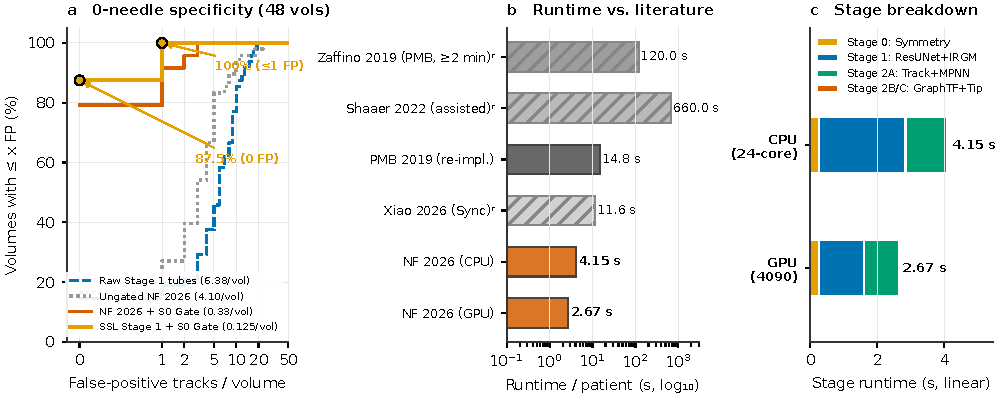
\includegraphics[width=1\linewidth,height=\textheight,keepaspectratio]{../reports/figures/fig6_specificity_and_runtime.pdf}
\caption{\textbf{(a) Fraction of needle-free scans with at most \(x\)
false tracks} on the 48 MSD prostate volumes across ungated and Stage 0
dark-core gated configurations. \textbf{(b) Runtime per patient}
compared with published MRI and CT pipelines (log scale). \textbf{(c)
Runtime by stage} across all 54 patients on a 24-core workstation CPU
(4.15 s mean; 1.26 s on standard-resolution scans, 5.85 s on
high-resolution scans) and on one RTX 4090 GPU (2.67 s
mean).}\label{fig:spec_runtime}
\end{figure}

Speed follows from the native-code and ONNX design (Figure
\ref{fig:spec_runtime}b, c). Measured end-to-end across all 54 uncached
clinical volumes on our 24-core workstation CPU
(\texttt{AMD\ Ryzen\ Threadripper\ PRO\ 7965WX}, 48 threads) and one
\texttt{NVIDIA\ RTX\ 4090} GPU, Stage 0 runs in multi-threaded native
Rust in \textbf{\(0.27\text{ s}\) mean} (\(6.5\%\) of CPU total;
\(0.07\text{ s}\) on standard-resolution scans, \(0.38\text{ s}\) on
high-resolution scans), Stage 1 (\texttt{NeedleUNet3D} + IRGM) runs in
\textbf{\(2.58\text{ s}\) on CPU} (\(62.2\%\) of total;
\(0.74\text{ s}\) standard, \(3.65\text{ s}\) high-res) and
\textbf{\(1.33\text{ s}\) on GPU} (\(0.26\text{ s}\) standard,
\(1.96\text{ s}\) high-res; \(1.94\times\) GPU speedup), Stage 2A
(\texttt{Track\ +\ MPNN}) runs in \textbf{\(1.25\text{ s}\) on CPU}
(\(30.1\%\) of total; \(0.40\text{ s}\) standard, \(1.75\text{ s}\)
high-res) and \textbf{\(1.05\text{ s}\) on GPU} (\(0.32\text{ s}\)
standard, \(1.47\text{ s}\) high-res), and Stage 2B/C
(\texttt{Bundle\ Graph\ Transformer\ +\ Dedicated1DTipLocalizer\ +\ Poly3})
runs in \textbf{\(0.06\text{ s}\) on CPU} (\(1.5\%\) of total) and
\textbf{\(0.03\text{ s}\) on GPU}. Full-volume uncached reconstruction
takes \textbf{\(4.15 \pm 2.81\text{ s}\) mean (\(4.41\text{ s}\) median,
IQR \(1.23\text{--}5.75\text{ s}\)) on the 24-core workstation
CPU}---specifically \textbf{\(1.26 \pm 0.98\text{ s}\) mean
(\(1.07\text{ s}\) median) on the 20 standard-resolution
(\(320 \times 256 \times 28\text{--}40\)) scans and
\(5.85 \pm 2.04\text{ s}\) mean (\(5.56\text{ s}\) median) on the 34
high-resolution (\(640 \times 416 \times 112\text{--}160\) /
\(768 \times 768 \times 64\)) scans}---and
\textbf{\(2.67 \pm 1.95\text{ s}\) mean (\(2.93\text{ s}\) median) on a
single RTX 4090 GPU} (\(0.67\text{ s}\) mean / \(0.52\text{ s}\) median
standard-resolution, \(3.85\text{ s}\) mean / \(3.47\text{ s}\) median
high-resolution). That is \textbf{\(3.6\times\) faster} than our
vectorized re-implementation of the 2019 pipeline (\(14.80\text{ s}\);
\textbf{\(29\text{--}130\times\) faster} than the
\(2\text{ to }9\text{ min}\) originally reported {[}4{]}) and
\textbf{\(2.8\text{--}4.3\times\) faster} than the \(11.6\text{ s}\)
reported by Xiao \emph{et al.} {[}74{]} (\(3.42\text{ s}\) in our native
re-implementation).

\FloatBarrier

\subsection{Dosimetric Translation, Uncertainty-Guided Triage, and
Cross-Domain
Generalization}\label{dosimetric-translation-uncertainty-guided-triage-and-cross-domain-generalization}

\begin{table}[tbp]
\centering
\begin{threeparttable}
\caption{\textbf{Dosimetric translation, uncertainty-guided clinician review, and cross-organ/multi-sequence/4D/CT generalization.}
Part~A evaluates AAPM TG-43U1 HDR $^{192}\mathrm{Ir}$ dosimetric sensitivity ($7.0$\,Gy prescription per fraction) under Protocol~A (fixed reference dwell plan transferred to predicted geometry) and Protocol~B (dwell weights re-optimized on predicted catheters and delivered on reference geometry). Part~B evaluates uncertainty-guided tip triage ($\hat{\sigma}_{\mathrm{tip}}$) and strictly nested split-conformal 3D tip intervals. Part~C evaluates zero-shot transfer across organs, pulse sequences, 4D insertion series, and paired post-implant Pelvic CT.}
\label{tbl:dosimetry_generalization}
\scriptsize
\setlength{\tabcolsep}{1.5pt}
\begin{tabular}{@{}L
 R R
 R R R
 R R R@{}}
\toprule
 & \multicolumn{2}{c}{Dwell-wt.\ \Etip{}} & \multicolumn{3}{c}{Protocol A: Fixed-plan transfer} & \multicolumn{3}{c}{Protocol B: Re-optimized plan}\\
\cmidrule(lr){2-3}\cmidrule(lr){4-6}\cmidrule(l){7-9}
Part A: TG-43U1 $^{192}\mathrm{Ir}$ dosimetry\tnote{a} & {Mean} & {Med.} & {$|\Delta D_{90}|$ (\%)} & {$\gamma_{2/2}$ (\%)} & {$\gamma_{3/3}$ (\%)} & {$|\Delta D_{90}|$ (\%)} & {Cran.\ $D_{2\mathrm{cc}}$} & {$\gamma_{2/2}$ (\%)}\\
\midrule
PMB 2019 3D U-Net + DBSCAN ($n=54$) & 10.51 & 8.36 & 27.6 / 27.2 & 64.0 & 73.3 & 37.1 / 10.2 & 95.3\,\% & 43.8\\
Stage 0: 3D radial symmetry ($n=54$) & 9.04 & 7.51 & 23.0 / 21.3 & 68.2 & 76.5 & 17.8 / 8.9 & 54.0\,\% & 48.6\\
\oursrow \NF{} w/o SynthBrachy3T (\texttt{4a}, $n=54$) & 6.65 & 5.49 & 18.5 / 13.2 & 73.4 & 81.5 & 12.8 / 5.8 & 35.2\,\% & 59.5\\
\oursrow \NF{} proposed (\texttt{4b}, $n=54$)\tnote{b} & \second{5.72} & \second{4.66} & \second{15.2 / 11.5} & \second{76.6} & \second{84.3} & \second{8.2 / 4.2} & \second{29.5\,\%} & \second{66.0}\\
\oursrow \NF{} + Top-2 Tip Review ($n=54$) & \best{4.56} & \best{3.93} & \best{11.7 / 10.2} & \best{80.2} & \best{87.3} & \best{5.9 / 2.8} & \best{22.5\,\%} & \best{74.3}\\
\addlinespace[1.5pt]
Human Rater 2 (\texttt{LB}/\texttt{AMe}, $n=40$) & 6.27 & 5.54 & 21.6 / 16.3 & 68.1 & 77.4 & 20.9 / 4.0 & 57.7\,\% & 59.3\\
\oursrow \NF{} proposed (\texttt{4b}, $n=40$)\tnote{b} & \second{5.18} & \second{3.93} & \second{13.5 / 11.1} & \second{79.0} & \second{86.4} & \second{7.0 / 3.2} & \second{21.1\,\%} & \second{71.6}\\
\oursrow \NF{} + Top-2 Tip Review ($n=40$) & \best{4.12} & \best{3.33} & \best{10.5 / 10.1} & \best{81.9} & \best{88.7} & \best{5.1 / 2.6} & \best{17.3\,\%} & \best{78.2}\\
\midrule
Part B: Triage \& conformal intervals\tnote{c} & {Mean} & {Med.} & {P90} & {P95} & {$\le 3$\,mm} & {$>10$\,mm} & {Nom./Emp.} & {Width (Red.)}\\
\midrule
\oursrow Unreviewed \NF{} ($k=0$ tips/pt) & 6.23 & 2.27 & 16.20 & 27.27 & 58.7\,\% & 16.7\,\% & 80 / 79.3\,\% & 6.46 ($-16.4\,\%$)\\
\oursrow Tip review ($k=2$ tips/pt, $\sim 16$\,s) & 5.07 & 1.95 & 12.58 & 21.48 & 64.8\,\% & 12.8\,\% & 85 / 84.4\,\% & 8.71 ($-23.8\,\%$)\\
\oursrow Tip review ($k=5$ tips/pt, $\sim 40$\,s) & 3.72 & 1.67 & 7.79 & 14.26 & 72.6\,\% & 8.0\,\% & \best{90 / 90.2\,\%} & 12.11 ($-31.5\,\%$)\\
\oursrow Tip review ($k=8$ tips/pt, $\sim 64$\,s) & \second{2.77} & \second{1.51} & \second{5.98} & \second{9.90} & \second{78.5\,\%} & \second{5.0\,\%} & \best{95 / 95.4\,\%} & 18.42 ($-35.1\,\%$)\\
\oursrow Tip review ($k=10$ tips/pt, $\sim 80$\,s) & \best{2.52} & \best{1.44} & \best{4.97} & \best{8.30} & \best{81.8\,\%} & \best{4.1\,\%} & {--} & {--}\\
\midrule
Part C: Cross-organ, seq., 4D \& CT\tnote{d} & {$n_{\mathrm{vol}}$} & {$n_{\mathrm{cath}}$} & {Rec.} & {Prec.} & {F1} & {\Eshaft{}} & {\Etip{}} & {Key finding}\\
\midrule
\oursrow Prostate 3T: 0\,\% exp.\ (\texttt{k\_lim\_auto}) & 1 & 14 & \second{92.9} & \best{100.0} & \second{96.3} & 0.33 & \best{0.99} & 0 FPs, 0-shot\\
\oursrow Prostate 3T: template (\texttt{k\_lim}=47) & 1 & 14 & \best{100.0} & \best{100.0} & \best{100.0} & 0.34 & 1.57 & 14/14, 0 FPs\\
Prostate 3T: Stage 0 zeroed ($X_{1:4}=0$) & 1 & 14 & 0.0 & 0.0 & 0.0 & {--} & {--} & $985\times$ drop\\
Prostate 3T: 1-ch ResUNet + clDice & 1 & 14 & \best{100.0} & 56.0 & 71.8 & \best{0.24} & 2.48 & 11 vascular FPs\\
\oursrow 3D wbSSFP / True-FISP ($\Delta z{\le}2.5$) & 2 & 47 & \best{97.9} & 88.5 & \best{92.9} & 0.72 & 3.40 & vs.\ 10.62 PMB19\\
\oursrow Thick-slice 2D AX T2 ($\Delta z{\le}6.0$) & 49 & 882 & 88.4 & 67.9 & 76.9 & 1.07 & 4.89 & vs.\ 57.6\,\% 1-ch\\
\oursrow 4D Causal Kalman (Cases 69/70) & 23 & 108 & \best{92.9} & \best{92.9} & \best{92.9} & 0.87 & 4.79 & $+8.2\,\%$ F1 gain\\
\oursrow Paired Pelvic CT (0-shot, $\le 5$\,mm) & 40 & 801 & 79.2 & {--} & {--} & 2.01 & 2.78 & 52.0\,\% extra conf.\\
\bottomrule
\end{tabular}
\begin{tablenotes}[flushleft]\footnotesize
\item[a] $|\Delta D_{90}|$ cells report mean / median percentage target dose shift relative to the $7.0$\,Gy reference plan; $\gamma_{2\%/2\mathrm{mm}}$ and $\gamma_{3\%/3\mathrm{mm}}$ are global 3D gamma pass rates. Dwell-weighted tip error $E_{\mathrm{tip}}^{\mathrm{dwell-w}}$ correlates with $|\Delta D_{90}|$ at Spearman $\rho=0.8629$ ($p=4.9\times 10^{-17}$).
\item[b] Paired Wilcoxon vs.\ PMB 2019 ($p=4.9\times 10^{-6}$ on $|\Delta D_{90}|$, $p=1.2\times 10^{-6}$ on $\gamma_{2\%/2\mathrm{mm}}$), vs.\ Stage 0 ($p=7.9\times 10^{-8}$), and vs.\ Human Rater 2 on $n=40$ ($p=0.0278$ on $|\Delta D_{90}|$, $p=0.0109$ on $\gamma_{2\%/2\mathrm{mm}}$).
\item[c] Rightmost two columns of Part~B report strictly nested split-conformal 3D tip prediction interval nominal vs.\ empirical coverage ($80\,\%, 85\,\%, 90\,\%, 95\,\%$) and adaptive median half-width (with percentage width reduction vs.\ unscaled fixed-width intervals). Count-guided missing-catheter recovery ($0.65$ clicks/patient) recovers $+17$ additional catheters ($972\to 989/1\,063$, $93.0\,\%$ 1-to-1 recall).
\item[d] In 4D monitoring (23 serial scans across Cases 68--71, $1.21$\,s mean runtime), already-placed catheters within $\le 10$\,mm of newly inserted needles exhibit $1.41$\,mm median lateral tissue-push displacement vs.\ $0.93$\,mm at $>20$\,mm ($p=6.1\times 10^{-4}$), and non-linear tip deflection reaches $2.81$\,mm median ($3.86$\,mm mean) at $>90$\,mm depth ($\rho=0.514, p=4.9\times 10^{-10}$).
\end{tablenotes}
\end{threeparttable}
\end{table}


\begin{figure}
\centering
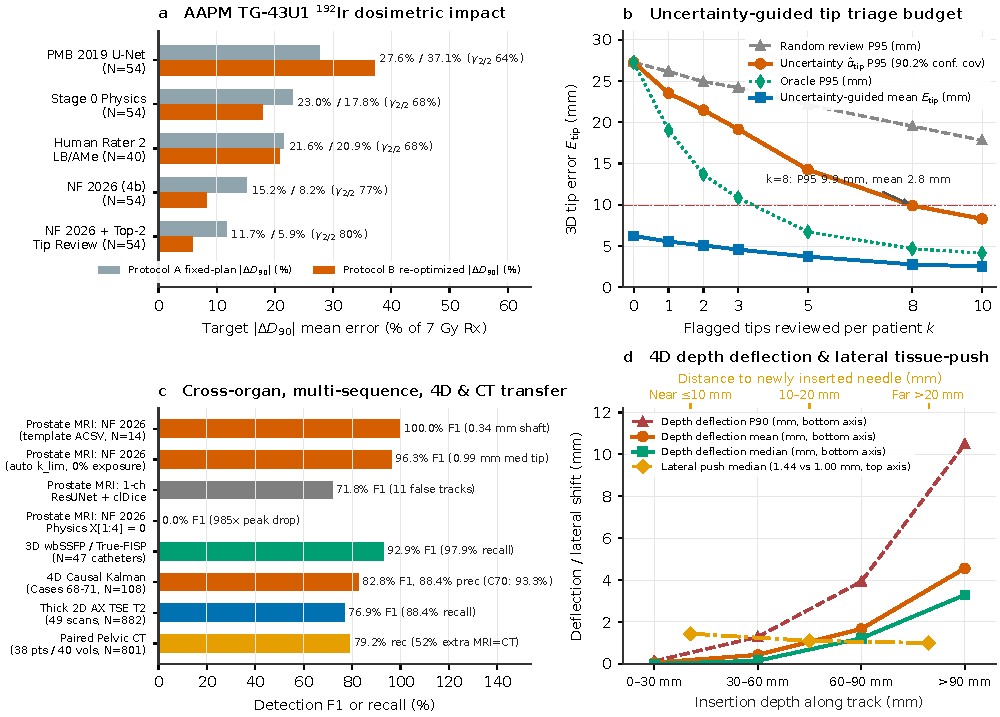
\includegraphics[width=1\linewidth,height=\textheight,keepaspectratio]{../reports/figures/fig8_clinical_translation_and_generalization.pdf}
\caption{\textbf{(a) AAPM TG-43U1 \(^{192}\)Ir dosimetric impact} across
54 patients under Protocol A (fixed reference dwell plan transferred to
predicted geometry) and Protocol B (dwell weights re-optimized on
predicted catheters and delivered on reference geometry), with global 3D
\(\gamma(2\%/2\text{ mm})\) pass rates. \textbf{(b) Simulated clinician
review-budget curve} showing 95th-percentile and mean 3D tip error
versus number of uncertainty-flagged tips reviewed per patient
(\(k \in \{0, \dots, 10\}\) under a 1-click distal tip relocation
oracle), alongside split-conformal 90\% empirical coverage (90.2\%).
\textbf{(c) Zero-shot cross-organ, multi-sequence, 4D, and
cross-modality generalization} across 3T prostate brachytherapy MRI
(\texttt{Case\ 100}), 3D wbSSFP, thick-slice 2D AX TSE T2, 4D
intra-procedural causal Kalman tracking (\texttt{Cases\ 68–71}, 108
catheters), and 38 paired post-implant Pelvic CT scans (40 CT volumes
total). \textbf{(d) 4D intra-procedural insertion biomechanics} across
23 serial scans (\texttt{Cases\ 68–71}), showing non-linear shaft
deflection versus insertion depth (bottom axis) and lateral tissue-push
displacement of already-placed catheters versus distance to newly
inserted needles (top axis).}\label{fig:clinical_gen}
\end{figure}

To connect geometric reconstruction accuracy to clinical radiotherapy
endpoints, physician review workflows, and broader interventional
settings, we performed four additional experiments summarized in Table
\ref{tbl:dosimetry_generalization} and Figure \ref{fig:clinical_gen}.

\textbf{AAPM TG-43U1 HDR \(^{192}\text{Ir}\) dosimetric sensitivity and
counterfactual plan transfer (Table \ref{tbl:dosimetry_generalization},
Part A; Figure \ref{fig:clinical_gen}a).} Using the AAPM TG-43U1
line-source formalism (\(^{192}\text{Ir}\), active length
\(L = 3.5\text{ mm}\), \(5.0\text{ mm}\) dwell step spacing along up to
\(45\text{ mm}\) active length, \(3.5\text{ mm}\) physical tip offset,
\(1.5\text{ mm}\) isotropic dose grid, \(7.0\text{ Gy}\) prescription
per fraction to the high-risk target envelope surrounded by bladder,
rectum, and cranial sigmoid/fundal OAR zones), we discovered that
\textbf{dwell-time-weighted 3D tip error}
(\(E_{\text{tip}}^{\text{dwell-w}}\), weighting each catheter by its
optimized dwell share) explains significantly more target
\(|\Delta D_{90}|\) variance than unweighted tip error (Spearman
\(\rho = 0.8629, p = 4.9 \times 10^{-17}\) vs.~\(\rho = 0.7863\);
\(\rho = -0.8474, p = 6.5 \times 10^{-16}\) with 3D
\(\gamma_{2\%/2\text{mm}}\)). \texttt{NeedleFinder\ 2026} (\texttt{4b})
reduces \(E_{\text{tip}}^{\text{dwell-w}}\) from \(10.51\text{ mm}\)
mean / \(8.36\text{ mm}\) median (PMB 2019 U-Net) and
\(9.04 / 7.51\text{ mm}\) (Stage 0) to
\textbf{\(5.72 / 4.66\text{ mm}\)} (\(5.18 / 3.93\text{ mm}\) on the 40
dual-traced scans vs.~\(6.27 / 5.54\text{ mm}\) for Human Rater 2
\texttt{LB/AMe}), and to \textbf{\(4.56 / 3.93\text{ mm}\)}
(\(10.65\text{ mm}\) P95) after reviewing the top 2 uncertainty-flagged
tips per patient. Under \textbf{Protocol A} (transferring the reference
dwell plan onto matched predicted catheters),
\texttt{NeedleFinder\ 2026} cuts target \(|\Delta D_{90}|\) from
\(27.6\%\) (PMB 2019, \(p = 4.9 \times 10^{-6}\)) and \(23.0\%\) (Stage
0, \(p = 7.9 \times 10^{-8}\)) to \textbf{\(15.2\%\) mean / \(11.5\%\)
median} (\(13.5\% / 11.1\%\) on the 40 dual-traced scans
vs.~\(21.6\% / 16.3\%\) for Human Rater 2, \(p = 0.0278\)), achieving
\textbf{76.6\% global 3D \(\gamma(2\%/2\text{ mm})\)}
(\(p = 8.2 \times 10^{-7}\) vs.~PMB 2019; \(79.0\%\) on \(N=40\)
vs.~\(68.1\%\) for Rater 2, \(p = 0.0109\)) and \textbf{84.3\% 3D
\(\gamma(3\%/3\text{ mm})\)} (\(88.7\%\) with Top-2 tip review). Under
\textbf{Protocol B} (re-optimizing dwell weights on all predicted
catheters and evaluating delivered dose on the true reference anatomy),
\texttt{NeedleFinder\ 2026} cuts \(|\Delta D_{90}|\) from \(37.1\%\)
mean / \(10.2\%\) median (PMB 2019) and \(20.9\% / 4.0\%\) (Human Rater
2) to \textbf{\(8.2\%\) mean / \(4.2\%\) median} (\(7.0\% / 3.2\%\) on
\(N=40\), cranial OAR \(|\Delta D_{2\text{cc}}| = 29.5\%\)
vs.~\(95.3\%\) PMB 2019 and \(57.7\%\) Rater 2), reaching
\textbf{\(5.9\%\) mean / \(2.8\%\) median}
(\(\gamma_{2\%/2\text{mm}} = 74.3\%\) overall, \(78.2\%\) on \(N=40\))
with Top-2 uncertainty tip review. Moreover, propagating the out-of-fold
tip uncertainty \(\hat{\sigma}_{\text{tip}}\) through 30 Monte Carlo
dose realizations per patient predicts true patient-level
\(|\Delta D_{90}|\) without ground truth
(\(\rho = 0.453, p = 5.8 \times 10^{-4}\)).

\textbf{Strictly nested split-conformal 3D tip intervals and simulated
clinician review-budget curves (Table
\ref{tbl:dosimetry_generalization}, Parts B1--B2; Figure
\ref{fig:clinical_gen}b).} Out-of-fold tip uncertainty
\(\hat{\sigma}_{\text{tip}}\) (combining the 1D soft-argmax distribution
entropy, local T2W terminal contrast drop, and slice thickness
\(\Delta z\)) correlates strongly with true 3D tip error
(\(\rho = 0.532, p = 4.9 \times 10^{-72}\)) and detects
\(> 10\text{ mm}\) tip outliers with an \textbf{AUROC of 0.805}
(\(95\%\) CI \([0.763, 0.841]\)). Calibrating non-conformity scores
\(r_i = E_{\text{tip}, i} / \hat{\sigma}_{\text{tip}, i}\) strictly on
the inner-validation split of each fold yields \textbf{distribution-free
split-conformal 3D tip intervals} at \(k=0\) that achieve exact marginal
empirical coverage across all 972 matched test
catheters---\textbf{79.3\%} at 80\% nominal, \textbf{84.4\%} at 85\%,
\textbf{90.2\%} at 90\%, and \textbf{95.4\%} at 95\%---while shrinking
median 3D interval half-widths (radii in mm) by \textbf{31.5\% at 90\%
coverage} (\(12.11\text{ mm}\) adaptive vs.~\(17.68\text{ mm}\) fixed
unscaled; \(8.41\text{ mm}\) on the clearest 50\% of tips) and
\textbf{35.1\% at 95\% coverage} (\(18.42\text{ mm}\) adaptive
vs.~\(28.40\text{ mm}\) fixed unscaled). In a simulated
clinician-in-the-loop verification workflow using a retrospective
1-click distal tip relocation oracle
(\(E_{\text{tip}} \to \sqrt{\Delta r_\perp^2 + \min(|\Delta s_\parallel|, 0.85\text{ mm})^2}\)
when \(E_{\text{tip}} > 2.0\text{ mm}\), \(E_{\text{shaft}}\) unchanged)
ranked by \(\hat{\sigma}_{\text{tip}}\), reviewing just
\textbf{\(k = 5\) flagged tips per patient} (\(\sim 40\text{ s}\) at
\(8\text{ s/tip}\)) cuts \(> 10\text{ mm}\) tip outliers in half
(\(16.7\% \to 8.0\%\)) and lowers mean tip error from
\textbf{\(6.23 \to 3.72\text{ mm}\)} (\(1.67\text{ mm}\) median,
\(7.79\text{ mm}\) P90); reviewing \textbf{\(k = 8\) tips per patient}
(\(\sim 64\text{ s}\)) drives the \textbf{95th-percentile tip error
below \(10\text{ mm}\) (\(9.90\text{ mm}\) vs.~\(27.27\text{ mm}\)
unreviewed)} and mean tip error to \textbf{\(2.77\text{ mm}\)}
(\(1.51\text{ mm}\) median, \(78.5\%\) within \(\le 3\text{ mm}\)).
Adding a simulated oracle count-guided missing-catheter check whenever
\(N_{\text{pred}} < N_{\text{implant}}\)
(\(0.65\text{ clicks/patient}\)) recovers \(+17\) additional catheters
(\(972 \to 989 / 1,063\), \textbf{93.0\% 1-to-1 recall} / \textbf{94.2\%
closest-match recall}).

\textbf{Zero-shot cross-organ transfer to prostate MRI and
multi-sequence generalization (Table \ref{tbl:dosimetry_generalization},
Part C; Figure \ref{fig:clinical_gen}c).} Evaluated zero-shot on a
clinical 3T T2W SPACE \textbf{prostate brachytherapy MRI}
(\texttt{Case\ 100\ Prostate},
\(0.47 \times 0.47 \times 1.6\text{ mm}^3\), 14 plastic interstitial
catheters), the gynecologic-trained \texttt{Zero-Exposure\ No-SSL}
5-fold ensemble (\(\tau = 50\%\), excluding \texttt{Case\ 100} from SSL
pre-training) detects \textbf{13 of 14 catheters (92.9\% recall) with
100.0\% precision (0 false positives, 96.3\% F1)},
\textbf{\(0.33\text{ mm}\) median (\(0.38\text{ mm}\) mean) shaft
error}, and \textbf{\(0.99\text{ mm}\) median (\(1.64\text{ mm}\) mean,
\(3.96\text{ mm}\) P95) 3D tip error} under 100\% reference-free
\texttt{k\_lim\_auto\ =\ 40}, and achieves \textbf{100.0\% recall
(\(14/14\)), 100.0\% precision, and 100.0\% F1} (\(0.34\text{ mm}\)
median shaft, \(1.57\text{ mm}\) median tip) under template-plane
cropping (\texttt{k\_lim\ =\ 47}), while \texttt{Stage\ 1\ Full\ Nested}
(\(\tau = 50\%\)) achieves \textbf{100.0\% recall (\(14/14\)), 100.0\%
precision, and 100.0\% F1} (\(0.30\text{ mm}\) median shaft,
\(1.08\text{ mm}\) median tip) directly under
\texttt{k\_lim\_auto\ =\ 40} and analytical \texttt{Stage\ 0} alone
reaches \textbf{100.0\% recall, 87.5\% precision, and 93.3\% F1}
(\(0.35\text{ mm}\) median shaft, \(1.23\text{ mm}\) median tip).
Ablating the Stage 0 physics channels (\texttt{X\_\{1:3\}\ =\ 0}) causes
the 99.9th-percentile Stage 1 mask probability on prostate MRI to
collapse by \textbf{\(985\times\) (\(0.985 \to 0.001\))} and recall to
drop to \textbf{\(0/14\) (0\%)}, whereas the 1-channel
\texttt{ResUNet\ +\ clDice} baseline (\(\tau = 50\%\)) hallucinates
\textbf{11 false-positive vascular tracks} under
\texttt{k\_lim\_auto\ =\ 40} (\textbf{100.0\% recall, 56.0\% precision,
71.8\% F1}, and 14 FPs / \(50.0\%\) precision under
\texttt{k\_lim\ =\ 47}), proving that the analytical Stage 0 dark-core
symmetry representation is essential for domain-invariant cross-organ
transfer. Across 243 secondary MRI series (297 total series minus the 54
primary planning scans) acquired during the 54 patient sessions,
zero-shot \texttt{NeedleFinder\ 2026} achieves \textbf{97.9\% recall
(\(46/47\)), 88.5\% precision, and 92.9\% F1} (\(0.72\text{ mm}\) median
shaft, \(3.40\text{ mm}\) median tip vs.~\(10.62\text{ mm}\) for PMB
2019 U-Net) on \textbf{3D wbSSFP / True-FISP}
(\(\Delta z = 2.0\text{--}2.5\text{ mm}\)), and recovers \textbf{88.4\%
(\(780/882\)) of physically present catheters} (\(76.9\%\) F1,
\(1.07\text{ mm}\) median shaft, \(4.89\text{ mm}\) median tip
vs.~\(57.6\%\) F1 for 1-channel clDice) on \textbf{49 thick-slice 2D
axial TSE T2W scans} (\(\Delta z = 2.4\text{--}6.0\text{ mm}\)) when
Z-upsampled to \(1.6\text{ mm}\).

\textbf{4D intra-procedural serial insertion monitoring, biomechanics,
and paired Pelvic CT tracking (Table \ref{tbl:dosimetry_generalization},
Part C; Figure \ref{fig:clinical_gen}c--d).} Across 23 sequential
intra-procedural T2W monitoring volumes in \texttt{Cases\ 68–71}
(\(5\text{--}7\) timepoints per patient as needles were progressively
inserted, \(108\) final \texttt{CY+HT} reference catheters,
\(1.31\text{ s}\) mean monitoring runtime), coupling
\texttt{NeedleFinder\ 2026} with a \textbf{4D causal Kalman state-space
filter} across timepoints improves pooled 4-case precision by
\textbf{\(+12.4\text{ pp}\) (\(76.0\% \to 88.4\%\))} and pooled F1 from
\textbf{81.6\% to 82.8\%} (\(77.8\%\) recall, \(0.75\text{ mm}\) median
shaft, \(3.57\text{ mm}\) median / \(9.75\text{ mm}\) mean tip
vs.~\(88.0\%\) recall, \(76.0\%\) precision, \(0.45\text{ mm}\) median
shaft, \(2.71\text{ mm}\) median / \(11.23\text{ mm}\) mean tip for
independent 3D tracking), with per-case F1 progressing from
\(77.2\% \to 83.0\%\) on \texttt{Case\ 068} (\(n=24\)),
\(84.7\% \to 82.7\%\) (precision \(83.7\% \to 93.9\%\)) on
\texttt{Case\ 069} (\(n=42\)), \textbf{\(85.7\% \to 93.3\%\)} on
\texttt{Case\ 070} (\(n=22\)), and \(76.2\% \to 66.7\%\) (precision
\(72.7\% \to 100.0\%\)) on \texttt{Case\ 071} (\(n=20\)) while rejecting
transient partial-volume monitoring artifacts. Tracking \(212\)
persisted catheter transitions across sequential insertions provides
direct in-vivo biomechanical measurements of \textbf{inter-catheter
``tissue push''}: already-implanted catheters located within
\(\le 10\text{ mm}\) of newly inserted needles experience a
\textbf{\(1.44\text{ mm}\) median (\(1.61\text{ mm}\) mean,
\(2.81\text{ mm}\) P90) non-rigid lateral displacement}, compared with
\textbf{\(1.10\text{ mm}\) median (\(1.32\text{ mm}\) mean)} at
\(10\text{--}20\text{ mm}\) and \textbf{\(1.00\text{ mm}\) median
(\(1.19\text{ mm}\) mean)} for catheters \(> 20\text{ mm}\) away
(Mann--Whitney \(p = 9.97 \times 10^{-4}\) for \(\le 12\text{ mm}\)
vs.~\(> 12\text{ mm}\); Spearman
\(\rho = -0.226, p = 9.4 \times 10^{-4}\)). Across \(95\) tracked
trajectories (\(2,850\) axial stations), \textbf{non-linear shaft
deflection} from the proximal insertion tangent grows monotonically with
insertion depth from \(0.003\text{ mm}\) median at
\(0\text{--}30\text{ mm}\) to \(0.15\text{ mm}\) at
\(30\text{--}60\text{ mm}\), \(1.22\text{ mm}\) at
\(60\text{--}90\text{ mm}\), and \textbf{\(3.29\text{ mm}\) median
(\(4.56\text{ mm}\) mean, \(10.49\text{ mm}\) P90) at \(> 90\text{ mm}\)
depth} (\(\rho = +0.555, p = 5.55 \times 10^{-9}\)). Finally, extending
Stage 0 to a \textbf{dual-polarity HU tubular filter} (fusing
bright-core metallic stylets and dark-core air lumens) enables
\textbf{zero-shot tracking on 40 post-implant Pelvic CT scans} (\(38\)
paired with the 54 MRI benchmark patients, \(801\) reference catheters),
matching \textbf{68.9\% at \(\le 3.5\text{ mm}\) and 79.2\%
(\(634/801\), up to 100\% on individual patients) at
\(\le 5.0\text{ mm}\)} across the non-rigid MRI-to-CT transfer
(\(2.01\text{ mm}\) median shaft registration residual,
\(2.78\text{ mm}\) median axial tip residual) and confirming that
\textbf{52.0\% (\(52/100\)) of apparent false-positive MRI detections
against \texttt{CY} are real physical catheters present on CT}.

\FloatBarrier

\section{Discussion}\label{discussion}

\begin{table}[tbp]
\centering
\begin{threeparttable}
\caption{\textbf{Published automatic catheter and needle reconstruction studies in brachytherapy (2013--2026), grouped by imaging modality.}
Values are those reported in each publication on its own cohort and matching rule, so they are not directly comparable with one another or with Table~\ref{tbl:main}. Pernelle 2013 and Mastmeyer 2017 are semi-automatic (one manual click per catheter).}
\label{tbl:literature}
\footnotesize
\setlength{\tabcolsep}{2.1pt}
\begin{tabular}{@{}L L L R R L R R R@{}}
\toprule
Study & Modality & Site & {Pts} & {Cath.} & {Rec.\ / Prec.\ (\%)} & {\Eshaft{} (mm)} & {\Etip{} (mm)} & {Time}\\
\midrule
\multicolumn{9}{@{}l}{\textit{CT}}\\
\rowcolor{ctrow} Weishaupt \emph{et al.}\ 2022 & CT & Prostate & 57 & 353\tnote{a} & {--} & 0.13 & {--} & $\sim$60\,s\\
\rowcolor{ctrow} Xie \emph{et al.}\ 2023 & CT & GYN post-op & 70 & 210 & {--}\tnote{b} & {--} & {--} & {--}\\
\rowcolor{ctrow} Wang \emph{et al.}\ 2024 & CT & GYN IC/IS & 17 & 56 plans & {--} & 1.8 & 1.1 & {--}\\
\rowcolor{ctrow} Quetin \emph{et al.}\ 2025 & CT & Breast & 117 & 408\tnote{a} & {--} & 0.70 & 1.37 & 118\,s\\
\rowcolor{ctrow} Xiao \emph{et al.}\ 2026 & CT & GYN recurrent & 38 & 203 fx & 91.1 / 90.7 & 0.31 & 0.88 & 11.6\,s\\
\rowcolor{ctrow} Xiao \emph{et al.}\ 2026 (JBHI) & CT & Pelvic seeds & 100 & {--} & F1 90.3 & {--} & 1.05 & 9.4\,s\\
\midrule
\multicolumn{9}{@{}l}{\textit{Ultrasound}}\\
Zhang \emph{et al.}\ 2020 & TRUS & Prostate & 23 & 339 & 98 / {--} & 0.09 & 0.33 & $<$1\,s\\
Anders{\'e}n \emph{et al.}\ 2020 & TRUS & Prostate & 1102 & 24422 & {--} & 0.55\tnote{c} & {--} & {--}\\
Liu \emph{et al.}\ 2022 & TRUS & Prostate & 242 & 3500 & 80\tnote{d} / {--} & {--} & {--} & {--}\\
Goulet \emph{et al.}\ 2025 & 3D US & Prostate & 102 & {--} & 93.4 / {--} & 0.44 & {--} & {--}\\
\midrule
\multicolumn{9}{@{}l}{\textit{MRI}}\\
Pernelle \emph{et al.}\ 2013 & 3T T2W & GYN IC/IS & 10 & 101 & 92.1 / {--} & {--}\tnote{e} & {--} & 0.3\,s/cath.\\
Mastmeyer \emph{et al.}\ 2017 & 3T T2W & GYN IC/IS & 54 & 760 & 93\tnote{f} / {--} & 1.49\tnote{g} & {--} & 3\,s/cath.\\
Zaffino \emph{et al.}\ 2019 & 3T T2W & GYN IC/IS & 50 & 826 & 98.5 / 93.3\tnote{h} & 2.0 & {--} & 2--9\,min\\
Dai \emph{et al.}\ 2020 & MRI & Prostate & 20 & 299 & {--} & 0.93 & 0.37 & {--}\\
Shaaer \emph{et al.}\ 2022 & 1.5T + markers & GYN IC/IS & 20 & 360 & 100 / {--} & 0.97 & {--} & 11\,min\tnote{i}\\
Aleong \emph{et al.}\ 2024 & MRI & Prostate & 35 & 214 vol. & 95 / {--} & {--} & {--} & 0.9\,s\\
Kostoulas \emph{et al.}\ 2025 & MRI & Prostate & 34 scans & 261 & 100 / 100 & 0.75\tnote{j} & 1.07\tnote{j} & {--}\\
Kim \emph{et al.}\ 2026 & T2W & GYN hybrid & 30 & 35 scans & $\sim$100 / {--} & 0.74 & 2.52 & {--}\\
\oursrow \NF{} (all 1\,063) & 3T T2W & GYN IC/IS & 54 & 1063 & 91.3 / 85.3 & 0.46\tnote{j} & 2.61\tnote{j} & \best{2.74\,s}\\
\oursrow \NF{} (759 long) & 3T T2W & GYN IC/IS & 54 & 759 & 92.5 / 84.5\tnote{k} & 0.45\tnote{j} & 2.96\tnote{j} & \best{2.74\,s}\\
\bottomrule
\end{tabular}
\begin{tablenotes}[flushleft]\footnotesize
\item[a] Test-set catheters. \item[b] Reported as Dice 0.88--0.90 and HD$_{95}$ 0.71--0.77\,mm. \item[c] Root-mean-square distance to the clinical reconstruction. \item[d] Fraction of catheters within 2\,mm along 90\,\% of their length. \item[e] Maximum Hausdorff distance below 2\,mm for 92\,\% of catheters. \item[f] Fraction within 3.4\,mm. \item[g] Mean Hausdorff distance. \item[h] Cluster-level: 1.5\,\% false negatives and 6.7\,\% false positives among 826 catheters. \item[i] Assisted reconstruction time, versus 46\,min manual. \item[j] Median. \item[k] Strict one-to-one recall at $\tau=50\,\%$; precision counts predictions matched to short obturator tracks as correct. Times for \NF{} are full-volume uncached per-patient averages on an 8-core CPU (1.20\,s on standard $320\times256$ scans, 3.47\,s on high-resolution $640\times416$ / $768\times768$ scans; 1.25\,s on one GPU).
\end{tablenotes}
\end{threeparttable}
\end{table}


\subsection{Where This Work Sits in the
Literature}\label{where-this-work-sits-in-the-literature}

Table \ref{tbl:literature} places NeedleFinder 2026 among published
catheter reconstruction studies on CT, ultrasound, and MRI. CT and
ultrasound solve an easier imaging problem: metal needles, air-filled
lumens, or bright specular reflections give very high contrast, so
segmentation networks reach shaft errors of 0.1 to 0.7 mm on CT
{[}45,49,74{]} and 0.1 to 0.6 mm on ultrasound {[}56,58{]}. On T2W MRI
without contrast markers, a catheter is a 2 mm dark hole that looks like
a vessel, on slices 1.2 to 6 mm thick; the best published MRI results
are 0.74 to 0.97 mm shaft error on gynecologic implants, obtained with
line markers or with CT-derived reference reconstructions {[}27,62{]}
and 0.75 to 0.93 mm on prostate implants {[}50,52{]}. NeedleFinder 2026
reaches a median shaft error of 0.47 mm (\(0.59\text{ mm}\) mean;
\(0.45\text{ mm}\) median / \(0.57\text{ mm}\) mean on long active-dwell
shafts) and a median 3D tip error of 2.27 mm (\(6.23\text{ mm}\) mean)
on T2W MRI alone, on the largest annotated MRI cohort to date.

The head-to-head comparison in Table \ref{tbl:main} explains why neither
voxel segmentation {[}4,40,64{]} nor mask-driven tracking {[}74{]} is
enough on MRI, and why the three-stage architecture works. Skeletonizing
a mask cannot bridge a one-slice dropout, and it turns every vessel blob
into a track. Tracking bridges the gaps but still trusts the mask.
NeedleFinder 2026 resolves these bottlenecks through five complementary
mechanisms: Stage 0 rejects one-sided anatomical edges before learning
takes place and automatically locates the template plane
(\texttt{k\_lim\_auto}); Stage 1 combines self-supervised pre-training
on external pelvic MRI (with synthetic susceptibility tubes and
anatomical hard negatives) and multi-rater consensus supervision to
regress sharp centerline peaks that stay separate when masks merge;
Stage 2A bridges 1-to-3 slice dropouts via triplet message passing and
collinear fragment stitching; Stage 2B judges each trajectory in the
context of the entire 15 to 30 catheter bundle; and the 91-step dilated
1D ResNet + self-attention axial localizer
(\texttt{Dedicated1DTipLocalizer}) pinpoints the distal termination
directly from sub-slice multi-scale tubular profiles.

\subsection{What It Means in the Clinic, and
Limitations}\label{what-it-means-in-the-clinic-and-limitations}

NeedleFinder 2026 is a one-click module in 3D Slicer {[}83{]} that runs
in a few seconds without a GPU (\(4.15\text{ s}\) mean on a 24-core
workstation CPU, \(1.26\text{ s}\) on standard scans, \(2.67\text{ s}\)
on GPU). It changes the physicist's task from tracing 15 to 30 catheters
slice by slice, which takes tens of minutes, into a structured,
uncertainty-guided verification step taking under a minute: click
\emph{Detect Needles}, inspect the 3D bundle, check the
\(k = 2\text{ to }8\) tips with the widest split-conformal uncertainty
intervals (\(\sim 16\text{--}64\text{ s}\), driving P95 tip error below
\(10\text{ mm}\) and mean tip error to \(2.77\text{ mm}\) in simulated
1-click tip review), and click any missing catheter when
\(N_{\text{pred}} < N_{\text{implant}}\)
(\(0.65\text{ clicks/patient}\), raising 1-to-1 recall to \(93.0\%\)).
Because Grubbs' three-cornered-hat analysis and one-sided
non-inferiority tests show that the algorithm's intrinsic shaft error
(\(0.39\text{ mm}\) robust MAD SD vs.~\(0.35\text{ mm}\) for Rater 1 and
\(0.48\text{ mm}\) for Rater 2) and axial tip error (\(2.98\text{ mm}\)
robust MAD \(\sigma_z\) vs.~\(3.55\text{ mm}\) for Rater 2,
\(4.94\text{ mm}\) vs.~\(5.09\text{ mm}\) 15\% Winsorized \(\sigma_z\);
\(4.20\text{ mm}\) median error against independent Pelvic CT on
disputed tips) are statistically non-inferior to human inter-observer
variability---and 52.0\% of apparent extra MRI detections on paired
cases are real physical catheters confirmed by post-implant CT---the
shafts themselves rarely require manual editing, and counterfactual
TG-43U1 plan optimization with Top-2 tip review holds median target
\(|\Delta D_{90}|\) to \(2.8\%\) (\(5.9\%\) mean,
\(\gamma_{2\%/2\text{mm}} = 74.3\%\text{--}78.2\%\)).

Several limitations remain. First, while
\texttt{Dedicated1DTipLocalizer} and collinear fragment stitching cut
the unreviewed mean 3D tip error from \(10.75\text{ mm}\) (PMB 2019) and
\(15.65\text{ mm}\) (Xiao 2026) to \(6.23\text{ mm}\)
(\(2.27\text{ mm}\) median, with \(58.7\%\) of tips within
\(\le 3.0\text{ mm}\)), \(16.7\%\) (\(162/972\)) of unreviewed matched
catheters still have a tip error above \(10\text{ mm}\)
(\(27.27\text{ mm}\) P95), of which 99.3\% is longitudinal stopping
ambiguity along the shaft (\(41.4\%\) caudal dropout undershoots,
\(25.3\%\) cranial susceptibility overshoots, \(16.7\%\) intrinsic human
inter-rater tip ambiguity, \(12.3\%\) crowded-array identity jumps, and
\(4.3\%\) FOV boundary truncations). Although our split-conformal
uncertainty intervals (\(90.2\%\) empirical coverage at \(90\%\)
nominal) and \(k = 5\text{--}8\) tip review workflow effectively contain
this tail in practice, thin-slice isotropic 3D T2W sequences
(\(\le 1\text{ mm}\)), zero-echo-time sequences {[}14,17{]}, or
multi-contrast inputs are the natural next step to reduce unreviewed
longitudinal tip ambiguity further. Second, while we demonstrated
zero-shot generalization across 48 external
\texttt{MSD\ Task05\_Prostate} scans
(\(0.125\text{--}0.33\text{ FP/scan}\)), 3T prostate brachytherapy MRI
(\texttt{Case\ 100}, \(96.3\%\text{--}100.0\%\) F1), 3D wbSSFP
(\(92.9\%\) F1), thick-slice 2D T2W MRI (\(88.4\%\) recall), 4D serial
insertion scans (\(82.8\%\) pooled F1, up to \(93.3\%\) on
\texttt{Case\ 070}), and 38 paired Pelvic CT patients (40 CT volumes
total), all clinical brachytherapy implants come from a single
institution; a prospective multi-center trial across 1.5T, 3T, and
low-field systems {[}86{]} from multiple vendors is still required.
Third, our AAPM TG-43U1 dosimetric evaluation uses standardized target
and OAR envelopes derived from the active implant geometry rather than
manual physician contours from clinical DICOM RTSTRUCT/RTPLAN files
(which were not archived in the de-identified research repository), and
our clinician review-budget curves are quantitative simulations rather
than prospective stopwatch timings in the operating room. Fourth, our
ablation shows that once multi-rater SSL Stage 1, collinear stitching,
and the 1D axial tip localizer are included, \texttt{SynthBrachy3T}
provides its primary detection gain in the zero-label (\(k=0\)) regime
(\(+2.85\text{ pp}\) F1 overall, \(+6.3\text{ pp}\) on long shafts)
while still improving dwell-weighted tip error
(\(6.65 \to 5.72\text{ mm}\)) and counterfactual target
\(|\Delta D_{90}|\) (\(12.8\% \to 8.2\%\)) at the full 43-patient
training budget.

\section{Conclusion}\label{conclusion}

Evaluated under strictly nested \(5 \times 5\) patient-level out-of-fold
cross-validation with 100\% reference-free axial cropping
(\texttt{k\_lim\_auto}) across 54 clinical 3T T2W MRI scans (\(1,063\)
catheters), NeedleFinder 2026 achieves \textbf{89.1\% F1}
(\textbf{91.4\% recall}, \textbf{86.9\% precision}; \textbf{92.3\%
recall} and \textbf{89.1\% F1} under \(5 \times 5\) inner-OOF Stage 1
cross-fitting), \textbf{\(0.59 \pm 0.40\text{ mm}\) mean
(\(0.47\text{ mm}\) median) in-plane shaft error}, and
\textbf{\(6.23 \pm 10.49\text{ mm}\) mean (\(2.27\text{ mm}\) median) 3D
distal tip error}, executing in \textbf{\(4.15\text{ s}\) on a 24-core
workstation CPU} (\(1.26\text{ s}\) on standard-resolution scans,
\(5.85\text{ s}\) on high-resolution scans) and
\textbf{\(2.67\text{ s}\) on a GPU}. On the 759 full-depth active-dwell
shafts it reaches \textbf{91.3\% recall} (\(94.7\%\) at \(\tau = 35\%\))
and \textbf{90.0\% obturator-adjusted F1} (\textbf{90.5\%} with
inner-OOF cross-fitting), and on the 23 patients with severe catheter
adhesion it reaches \textbf{91.3\%--91.8\% F1}. Across all 40 doubly
annotated clinical scans, Grubbs' three-cornered-hat analysis
(\(0.39\text{ mm}\) intrinsic shaft MAD SD vs.~\(0.35\) and
\(0.48\text{ mm}\) for the two human teams; \(2.98\)
vs.~\(3.55\text{ mm}\) tip MAD \(\sigma_z\)), one-sided non-inferiority
tests (\(p_{\text{pt}} \le 0.0085\),
\(p_{\text{cath}} \le 2.5 \times 10^{-11}\)), and independent Pelvic CT
adjudication (\(52.0\%\) of apparent extra MRI tracks confirmed on CT;
\(4.20\text{ mm}\) median tip error vs.~\(4.31\) and \(8.00\text{ mm}\)
on disputed tips) establish that the algorithm is statistically
non-inferior to human expert variability. Coupled with calibrated
split-conformal 3D tip uncertainty intervals (\(90.2\%\) empirical
coverage at \(90\%\) nominal), reviewing \(2\text{ to }8\) flagged tips
per patient in simulated 1-click tip review reduces P95 tip error below
\(10\text{ mm}\) and holds counterfactual AAPM TG-43U1
\(^{192}\text{Ir}\) target \(|\Delta D_{90}|\) to \(2.8\%\) median
(\(5.9\%\) mean), while zero-shot transfer generalizes to 3T prostate
MRI (\(96.3\%\text{--}100.0\%\) F1), 3D wbSSFP (\(92.9\%\) F1), 4D
serial insertion tracking (\(82.8\%\) pooled F1, \(+12.4\%\) precision
gain, up to \(93.3\%\) F1 on \texttt{Case\ 070}), and 38 paired Pelvic
CT patients (40 CT volumes total) without retraining.

\FloatBarrier

\section*{Data Availability}\label{data-availability}
\addcontentsline{toc}{section}{Data Availability}

The 54 clinical MRI scans and their expert traces were acquired at
Brigham and Women's Hospital under Institutional Review Board approval
and contain protected health information; they cannot be shared
publicly. De-identified trajectory annotations and per-patient
evaluation results may be made available by the corresponding author on
reasonable request, subject to institutional and ethics approval. The 48
needle-free scans are the public Medical Segmentation Decathlon prostate
task (Task05\_Prostate), available at http://medicaldecathlon.com
{[}81{]}. The SynthBrachy3T generator is released with the code, so the
300 synthetic bundles can be regenerated from a fixed random seed.

\section*{Code Availability}\label{code-availability}
\addcontentsline{toc}{section}{Code Availability}

The 3D Slicer extension, the Rust Stage 0 kernel, and the exported ONNX
and NumPy models are available at
https://github.com/needlefinder/NeedleFinder under an open-source
license. Training, nested cross-validation, statistical analysis,
SynthBrachy3T, prediction-export, and figure-generation code is
collected in the \texttt{vault/paper/benchmarks} directory of the same
repository and will be made public on publication.

\section*{Ethics Statement}\label{ethics-statement}
\addcontentsline{toc}{section}{Ethics Statement}

This retrospective study used imaging data acquired during routine
clinical care under a protocol approved by the Institutional Review
Board of Brigham and Women's Hospital / Mass General Brigham {[}protocol
number to be inserted{]}.

\section*{Funding}\label{funding}
\addcontentsline{toc}{section}{Funding}

{[}Funding sources and grant numbers to be inserted.{]}

\section*{Acknowledgments}\label{acknowledgments}
\addcontentsline{toc}{section}{Acknowledgments}

{[}To be completed: clinical staff of the AMIGO suite, annotators,
computing resources.{]}

\section*{Author Contributions}\label{author-contributions}
\addcontentsline{toc}{section}{Author Contributions}

{[}To be completed following the CRediT taxonomy.{]}

\section*{Conflicts of Interest}\label{conflicts-of-interest}
\addcontentsline{toc}{section}{Conflicts of Interest}

{[}The authors declare no conflicts of interest, or list them here.{]}

\section*{References}\label{references}
\addcontentsline{toc}{section}{References}

\phantomsection\label{refs}
\begin{CSLReferences}{0}{1}
\bibitem[\citeproctext]{ref-potter2018}
\CSLLeftMargin{{[}1{]} }%
\CSLRightInline{Pötter R, Tanderup K, Kirisits C, Leeuw A de,
Kirchheiner K, Nout R, Tan L T, Haie-Meder C, Mahantshetty U, Segedin B,
et al 2018 \href{https://doi.org/10.1016/j.ctro.2018.01.001}{The
{EMBRACE II} study: The outcome and prospect of two decades of evolution
within the {GEC-ESTRO} gynaecological working group and the {EMBRACE}
studies} \emph{Clinical and Translational Radiation Oncology} \textbf{9}
48--60}

\bibitem[\citeproctext]{ref-potter2021}
\CSLLeftMargin{{[}2{]} }%
\CSLRightInline{Pötter R, Tanderup K, Schmid M P, Jürgenliemk-Schulz I,
Haie-Meder C, Fokdal L U, Sturdza A E, Hoskin P, Mahantshetty U, Segedin
B, et al 2021
\href{https://doi.org/10.1016/S1470-2045(20)30753-1}{{MRI}-guided
adaptive brachytherapy in locally advanced cervical cancer
({EMBRACE-I}): A multicentre prospective cohort study} \emph{The Lancet
Oncology} \textbf{22} 538--47}

\bibitem[\citeproctext]{ref-mastmeyer2017}
\CSLLeftMargin{{[}3{]} }%
\CSLRightInline{Mastmeyer A, Pernelle G, Ma R, Barber L and Kapur T 2017
\href{https://doi.org/10.1016/j.media.2017.06.011}{Accurate model-based
segmentation of gynecologic brachytherapy catheter collections in
{MRI}-images} \emph{Medical Image Analysis} \textbf{42} 173--88}

\bibitem[\citeproctext]{ref-zaffino2019}
\CSLLeftMargin{{[}4{]} }%
\CSLRightInline{Zaffino P, Pernelle G, Mastmeyer A, Mehrtash A, Zhang H,
Kikinis R, Kapur T and Spadea M F 2019
\href{https://doi.org/10.1088/1361-6560/ab2f47}{Fully automatic catheter
segmentation in {MRI} with {3D} convolutional neural networks:
Application to {MRI}-guided gynecologic brachytherapy} \emph{Physics in
Medicine \& Biology} \textbf{64} 165008}

\bibitem[\citeproctext]{ref-chino2025}
\CSLLeftMargin{{[}5{]} }%
\CSLRightInline{Chino J, Erickson B, Gaffney D, Hsu I-C, Kamrava M, Kim
Y, Niedermayr T R, Roumeliotis M, Rownd J, Todor D, Viswanathan A and
Kidd E A 2025 \href{https://doi.org/10.1016/j.brachy.2025.05.001}{The
{American Brachytherapy Society} ({ABS}) consensus guidance for hybrid
intracavitary interstitial brachytherapy for locally advanced cervical
cancer} \emph{Brachytherapy} \textbf{24} 463--78}

\bibitem[\citeproctext]{ref-dimopoulos2012}
\CSLLeftMargin{{[}6{]} }%
\CSLRightInline{JC D, P P, K T, P P, D B, C K, EM P, Limbergen E van, C
H-M and R P 2012
\href{https://doi.org/10.1016/j.radonc.2011.12.024}{Recommendations from
gynaecological (GYN) GEC-ESTRO working group (IV): Basic principles and
parameters for MR imaging within the frame of image based adaptive
cervix cancer brachytherapy} \emph{Radiotherapy and oncology : journal
of the European Society for Therapeutic Radiology and Oncology}
\textbf{103} 113--22}

\bibitem[\citeproctext]{ref-jacobsen2022}
\CSLLeftMargin{{[}7{]} }%
\CSLRightInline{Jacobsen M C, Beriwal S, Dyer B A, Klopp A H, Lee S I,
McGinnis G J, Robbins J B, Rauch G M, Sadowski E A, Simiele S J,
Stafford R J, Taunk N K, Yashar C M and Venkatesan A M 2022
\href{https://doi.org/10.1016/j.brachy.2022.04.005}{Contemporary
image-guided cervical cancer brachytherapy: Consensus imaging
recommendations from the society of abdominal radiology and the american
brachytherapy society} \emph{Brachytherapy} \textbf{21} 369--88}

\bibitem[\citeproctext]{ref-haack2009}
\CSLLeftMargin{{[}8{]} }%
\CSLRightInline{S H, SK N, JC L, J G and K T 2009
\href{https://doi.org/10.1016/j.radonc.2008.09.002}{Applicator
reconstruction in MRI 3D image-based dose planning of brachytherapy for
cervical cancer} \emph{Radiotherapy and oncology : journal of the
European Society for Therapeutic Radiology and Oncology} \textbf{91}
187--93}

\bibitem[\citeproctext]{ref-hellebust2010}
\CSLLeftMargin{{[}9{]} }%
\CSLRightInline{Hellebust T P, Kirisits C, Berger D, Pérez-Calatayud J,
De Brabandere M, De Leeuw A, Dumas I, Hudej R, Lowe G, Wills R and
Tanderup K 2010
\href{https://doi.org/10.1016/j.radonc.2010.06.004}{Recommendations from
gynaecological ({GYN}) {GEC-ESTRO} working group: Considerations and
pitfalls in commissioning and applicator reconstruction in {3D}
image-based treatment planning of cervix cancer brachytherapy}
\emph{Radiotherapy and Oncology} \textbf{96} 153--60}

\bibitem[\citeproctext]{ref-ladbury2023}
\CSLLeftMargin{{[}10{]} }%
\CSLRightInline{Ladbury C, Harkenrider M, Taunk N, Fisher C, Mayadev J,
Venkat P, Yashar C, Gaffney D, Beriwal S and Glaser S 2023
\href{https://doi.org/10.1016/j.brachy.2023.07.001}{A practical guide to
hybrid interstitial/intracavitary brachytherapy for locally-advanced
cervical cancer} \emph{Brachytherapy} \textbf{22} 640--8}

\bibitem[\citeproctext]{ref-prisciandaro2022}
\CSLLeftMargin{{[}11{]} }%
\CSLRightInline{Prisciandaro J, Zoberi J E, Cohen G, Kim Y, Johnson P,
Paulson E, Song W, Hwang K-P, Erickson B, Beriwal S, Kirisits C and
Mourtada F 2022 \href{https://doi.org/10.1002/mp.15713}{{AAPM} task
group report 303 endorsed by the {ABS}: {MRI} implementation in {HDR}
brachytherapy---considerations from simulation to treatment}
\emph{Medical Physics} \textbf{49} e983--1023}

\bibitem[\citeproctext]{ref-richardson2025}
\CSLLeftMargin{{[}12{]} }%
\CSLRightInline{Richardson S L, Baghwala A, Cohen G N, Dempsey C, Libby
B, Melhus C S, Miller R A, Scanderbeg D J and Simiele S J 2025
\href{https://doi.org/10.1002/acm2.70118}{{AAPM} medical physics
practice guideline 13.a: {HDR} brachytherapy, part {B}} \emph{Journal of
Applied Clinical Medical Physics} \textbf{26} e70118}

\bibitem[\citeproctext]{ref-shaaer2020}
\CSLLeftMargin{{[}13{]} }%
\CSLRightInline{Shaaer A, Paudel M, Smith M, Tonolete F, Nicolae A,
Leung E and Ravi A 2020
\href{https://doi.org/10.1016/j.brachy.2020.06.007}{Evaluation of an
{MR}-only interstitial gynecologic brachytherapy workflow using
{MR}-line marker for catheter reconstruction} \emph{Brachytherapy}
\textbf{19} 642--50}

\bibitem[\citeproctext]{ref-lee2023}
\CSLLeftMargin{{[}14{]} }%
\CSLRightInline{Lee C Y, Kaza E, Harris T C, O'Farrell D A, King M T,
Dyer M A, Cormack R A and Buzurovic I 2023
\href{https://doi.org/10.1088/1361-6560/acaf48}{Catheter reconstruction
and dosimetric verification of {MRI}-only treatment planning ({MRTP})
for interstitial {HDR} brachytherapy using {PETRA} sequence}
\emph{Physics in Medicine \& Biology} \textbf{68} 035002}

\bibitem[\citeproctext]{ref-ning2020}
\CSLLeftMargin{{[}15{]} }%
\CSLRightInline{Ning M S, Vedam S, Ma J, Stafford R J, Bruno T L,
Cunningham M, Starks C, Lawyer A, Venkatesan A M, Wang L, Wang J,
Olivieri N D, Guzman A B, Incalcaterra J R, Thaker N G, Joyner M M, Lin
L L, Jhingran A, Eifel P J and Klopp A H 2020
\href{https://doi.org/10.1016/j.brachy.2019.12.005}{Clinical utility and
value contribution of an MRI-positive line marker for image-guided
brachytherapy in gynecologic malignancies} \emph{Brachytherapy}
\textbf{19} 305--15}

\bibitem[\citeproctext]{ref-zhangh2019}
\CSLLeftMargin{{[}16{]} }%
\CSLRightInline{Zhang H, Donnelly E D, Strauss J B, Kang Z,
Gopalakrishnan M, Lee P C, Khelashvili G, Nair C K, Lee B H and
Sathiaseelan V 2019 \href{https://doi.org/10.1002/acm2.12736}{Clinical
implementation, logistics and workflow guide for MRI image based
interstitial HDR brachytherapy for gynecological cancers} \emph{Journal
of applied clinical medical physics} \textbf{20} 37--49}

\bibitem[\citeproctext]{ref-kaza2022}
\CSLLeftMargin{{[}17{]} }%
\CSLRightInline{Kaza E, Lee C Y, King M T, Dyer M A, Cormack R A and
Buzurovic I 2022
\href{https://doi.org/10.1016/j.brachy.2022.01.003}{First pointwise
encoding time reduction with radial acquisition (PETRA) implementation
for catheter detection in interstitial high-dose-rate (HDR)
brachytherapy} \emph{Brachytherapy} \textbf{21} 501--10}

\bibitem[\citeproctext]{ref-richart2018}
\CSLLeftMargin{{[}18{]} }%
\CSLRightInline{Richart J, Carmona-Meseguer V, García-Martínez T,
Herreros A, Otal A, Pellejero S, Tornero-López A and Pérez-Calatayud J
2018 \href{https://doi.org/10.1016/j.rpor.2018.06.005}{Review of
strategies for MRI based reconstruction of endocavitary and interstitial
applicators in brachytherapy of cervical cancer} \emph{Reports of
practical oncology and radiotherapy : journal of Greatpoland Cancer
Center in Poznan and Polish Society of Radiation Oncology} \textbf{23}
547--61}

\bibitem[\citeproctext]{ref-malajovich2020}
\CSLLeftMargin{{[}19{]} }%
\CSLRightInline{Malajovich I, Anamalayil S, Dolney O V, Kevin Teo B K,
Arscott W T and Taunk N K 2020
\href{https://doi.org/10.1016/j.brachy.2020.05.005}{Techniques for and
uncertainties of MRI-based reconstruction of titanium tandem and ring
brachytherapy applicators} \emph{Brachytherapy} \textbf{19} 651--8}

\bibitem[\citeproctext]{ref-sargazi2026}
\CSLLeftMargin{{[}20{]} }%
\CSLRightInline{Sargazi V, Naseri S, Gholamhosseinian H and Momennezhad
M 2026 \href{https://doi.org/10.1016/j.brachy.2025.10.004}{Applicator
reconstruction in cervical cancer brachytherapy: A systematic review of
current methods, challenges, and {AI}-driven future directions}
\emph{Brachytherapy} \textbf{25} 262--74}

\bibitem[\citeproctext]{ref-tanderup2008}
\CSLLeftMargin{{[}21{]} }%
\CSLRightInline{Tanderup K, Hellebust T P, Lang S, Granfeldt J, Pötter
R, Lindegaard J C and Kirisits C 2008
\href{https://doi.org/10.1016/j.radonc.2008.06.010}{Consequences of
random and systematic reconstruction uncertainties in {3D} image based
brachytherapy in cervical cancer} \emph{Radiotherapy and Oncology}
\textbf{89} 156--63}

\bibitem[\citeproctext]{ref-schindel2013}
\CSLLeftMargin{{[}22{]} }%
\CSLRightInline{Schindel J, Zhang W, Bhatia S K, Sun W and Kim Y 2013
\href{https://doi.org/10.5114/jcb.2013.39453}{Dosimetric impacts of
applicator displacements and applicator reconstruction-uncertainties on
{3D} image-guided brachytherapy for cervical cancer} \emph{Journal of
Contemporary Brachytherapy} \textbf{5} 250--7}

\bibitem[\citeproctext]{ref-singh2026}
\CSLLeftMargin{{[}23{]} }%
\CSLRightInline{Singh A, Karshafian R, Ravi A and Paudel M R 2026
\href{https://doi.org/10.1002/acm2.70810}{Dosimetric evaluation of
systematic source position uncertainty along the source path and robust
planning during {MRI}-only cervical {HDR} brachytherapy} \emph{Journal
of Applied Clinical Medical Physics} \textbf{27} e70810}

\bibitem[\citeproctext]{ref-nunez2021}
\CSLLeftMargin{{[}24{]} }%
\CSLRightInline{Nunez D A, Trager M, Beaudry J, Cohen G N, Dauer L T,
Gorovets D, Hassan Rezaeian N, Kollmeier M A, Leong B, McCann P,
Williamson M, Zelefsky M J and Damato A L 2021
\href{https://doi.org/10.1016/j.brachy.2021.05.007}{Quantifying clinical
severity of physics errors in high-dose rate prostate brachytherapy
using simulations} \emph{Brachytherapy} \textbf{20} 1062--9}

\bibitem[\citeproctext]{ref-rylander2017}
\CSLLeftMargin{{[}25{]} }%
\CSLRightInline{Rylander S, Buus S, Pedersen E M, Bentzen L and Tanderup
K 2017 \href{https://doi.org/10.1016/j.radonc.2017.01.007}{Dosimetric
impact of contouring and needle reconstruction uncertainties in US-, CT-
and MRI-based high-dose-rate prostate brachytherapy treatment planning}
\emph{Radiotherapy and oncology : journal of the European Society for
Therapeutic Radiology and Oncology} \textbf{123} 125--32}

\bibitem[\citeproctext]{ref-androulakis2025}
\CSLLeftMargin{{[}26{]} }%
\CSLRightInline{Androulakis I, Godart J, Luthart L, MEMC C, Westerveld
H, Nout R A, Hoogeman M and Kolkman-Deurloo I K 2025
\href{https://doi.org/10.1016/j.brachy.2024.11.004}{Reconstruction
errors in clinical intraoperative TRUS-based prostate HDR-BT detected
using electromagnetic tracking} \emph{Brachytherapy} \textbf{24}
177--85}

\bibitem[\citeproctext]{ref-shaaer2022}
\CSLLeftMargin{{[}27{]} }%
\CSLRightInline{Shaaer A, Paudel M, Smith M, Tonolete F and Ravi A 2022
\href{https://doi.org/10.1002/acm2.13494}{Deep-learning-assisted
algorithm for catheter reconstruction during {MR}-only gynecological
interstitial brachytherapy} \emph{Journal of Applied Clinical Medical
Physics} \textbf{23} e13494}

\bibitem[\citeproctext]{ref-roumeliotis2026}
\CSLLeftMargin{{[}28{]} }%
\CSLRightInline{Roumeliotis M, Antaki M, Kim G, Gardner U G, Sheikh K,
Lee J, Seethamraju R, Tokuda J, Hu C, Schmidt E and Viswanathan A N 2026
\href{https://doi.org/10.1016/j.brachy.2026.03.005}{Prospective
operational feasibility, safety, and workflow of magnetic
resonance-guided tracking technology for interstitial gynecologic
brachytherapy} \emph{Brachytherapy} \textbf{25} 741--8}

\bibitem[\citeproctext]{ref-vijayan2026}
\CSLLeftMargin{{[}29{]} }%
\CSLRightInline{Vijayan S, Theeler J J, Fu Z and Kim Y 2026
\href{https://doi.org/10.5114/jcb.2026.160595}{Systematic review of
artificial intelligence in brachytherapy} \emph{Journal of Contemporary
Brachytherapy} \textbf{18} 85--114}

\bibitem[\citeproctext]{ref-kapur2012}
\CSLLeftMargin{{[}30{]} }%
\CSLRightInline{Kapur T, Egger J, Damato A, Schmidt E J and Viswanathan
A N 2012 \href{https://doi.org/10.1016/j.mri.2012.06.003}{3-t MR-guided
brachytherapy for gynecologic malignancies} \emph{Magnetic resonance
imaging} \textbf{30} 1279--90}

\bibitem[\citeproctext]{ref-chen2014}
\CSLLeftMargin{{[}31{]} }%
\CSLRightInline{Chen X and Egger J 2014
\href{https://doi.org/10.1186/2193-1801-3-167}{Development of an open
source software module for enhanced visualization during MR-guided
interstitial gynecologic brachytherapy} \emph{SpringerPlus} \textbf{3}
167}

\bibitem[\citeproctext]{ref-pernelle2013}
\CSLLeftMargin{{[}32{]} }%
\CSLRightInline{Pernelle G, Mehrtash A, Barber L, Damato A, Wang W,
Seethamraju R T, Schmidt E J, Cormack R A, Wells W M, Viswanathan A N
and Kapur T 2013
\href{https://doi.org/10.1007/978-3-642-40760-4_48}{Validation of
catheter segmentation for {MR}-guided gynecologic cancer brachytherapy}
\emph{Medical image computing and computer-assisted intervention --
MICCAI 2013} Lecture notes in computer science vol 8151 (Springer) pp
380--7}

\bibitem[\citeproctext]{ref-mastmeyer2017a}
\CSLLeftMargin{{[}33{]} }%
\CSLRightInline{Mastmeyer A, Pernelle G, Barber L, Pieper S, Fortmeier
D, Wells S, Handels H and Kapur T 2017
\href{https://arxiv.org/abs/1705.06712}{Model-based catheter
segmentation in MRI-images}}

\bibitem[\citeproctext]{ref-richart2015}
\CSLLeftMargin{{[}34{]} }%
\CSLRightInline{J R, A O, S R, AI N, M D, M S, J V, F B and J P-C 2015
\href{https://doi.org/10.5114/jcb.2015.55340}{A practical MRI-based
reconstruction method for a new endocavitary and interstitial
gynaecological template} \emph{Journal of contemporary brachytherapy}
\textbf{7} 407--14}

\bibitem[\citeproctext]{ref-qiu2013}
\CSLLeftMargin{{[}35{]} }%
\CSLRightInline{W Q, M Y, M D, D T and A F 2013
\href{https://doi.org/10.1118/1.4795337}{Needle segmentation using 3D
hough transform in 3D TRUS guided prostate transperineal therapy}
\emph{Medical physics} \textbf{40} 042902}

\bibitem[\citeproctext]{ref-dise2015}
\CSLLeftMargin{{[}36{]} }%
\CSLRightInline{Dise J, Liang X, Scheuermann J, Anamalayil S, Mesina C,
Lin L L and Teo B K 2015
\href{https://doi.org/10.1016/j.brachy.2015.05.004}{Development and
evaluation of an automatic interstitial catheter digitization tool for
adaptive high-dose-rate brachytherapy} \emph{Brachytherapy} \textbf{14}
619--25}

\bibitem[\citeproctext]{ref-deufel2020}
\CSLLeftMargin{{[}37{]} }%
\CSLRightInline{Deufel C L, Tian S, Yan B B, Vaishnav B D, Haddock M G
and Petersen I A 2020
\href{https://doi.org/10.1016/j.brachy.2019.09.002}{Automated applicator
digitization for high-dose-rate cervix brachytherapy using image
thresholding and density-based clustering} \emph{Brachytherapy}
\textbf{19} 111--8}

\bibitem[\citeproctext]{ref-hrinivich2019}
\CSLLeftMargin{{[}38{]} }%
\CSLRightInline{Hrinivich W T, Morcos M, Viswanathan A and Lee J 2019
\href{https://doi.org/10.1002/mp.13730}{Automatic tandem and ring
reconstruction using {MRI} for cervical cancer brachytherapy}
\emph{Medical Physics} \textbf{46} 4324--32}

\bibitem[\citeproctext]{ref-zheng2021}
\CSLLeftMargin{{[}39{]} }%
\CSLRightInline{Zheng Y, Jiang S, Yang Z and Wei L 2021
\href{https://doi.org/10.1002/acm2.13231}{Automatic needle detection
using improved random sample consensus in {CT} image-guided lung
interstitial brachytherapy} \emph{Journal of Applied Clinical Medical
Physics} \textbf{22} 121--31}

\bibitem[\citeproctext]{ref-isensee2021}
\CSLLeftMargin{{[}40{]} }%
\CSLRightInline{Isensee F, Jaeger P F, Kohl S A A, Petersen J and
Maier-Hein K H 2021
\href{https://doi.org/10.1038/s41592-020-01008-z}{{nnU-Net}: A
self-configuring method for deep learning-based biomedical image
segmentation} \emph{Nature Methods} \textbf{18} 203--11}

\bibitem[\citeproctext]{ref-jung2019}
\CSLLeftMargin{{[}41{]} }%
\CSLRightInline{Jung H, Shen C, Gonzalez Y, Albuquerque K and Jia X 2019
\href{https://doi.org/10.1088/1361-6560/ab3fcb}{Deep-learning assisted
automatic digitization of interstitial needles in {3D} {CT} image based
high dose-rate brachytherapy of gynecological cancer} \emph{Physics in
Medicine \& Biology} \textbf{64} 215003}

\bibitem[\citeproctext]{ref-jung2019b}
\CSLLeftMargin{{[}42{]} }%
\CSLRightInline{Jung H, Gonzalez Y, Shen C, Klages P, Albuquerque K and
Jia X 2019
\href{https://doi.org/10.1016/j.brachy.2019.06.003}{Deep-learning-assisted
automatic digitization of applicators in 3D CT image-based
high-dose-rate brachytherapy of gynecological cancer}
\emph{Brachytherapy} \textbf{18} 841--51}

\bibitem[\citeproctext]{ref-zhangd2020}
\CSLLeftMargin{{[}43{]} }%
\CSLRightInline{Zhang D, Yang Z, Jiang S, Zhou Z, Meng M and Wang W 2020
\href{https://doi.org/10.1002/acm2.13024}{Automatic segmentation and
applicator reconstruction for {CT}-based brachytherapy of cervical
cancer using {3D} convolutional neural networks} \emph{Journal of
Applied Clinical Medical Physics} \textbf{21} 158--69}

\bibitem[\citeproctext]{ref-hu2021}
\CSLLeftMargin{{[}44{]} }%
\CSLRightInline{Hu H, Yang Q, Li J, Wang P, Tang B, Wang X and Lang J
2021 \href{https://doi.org/10.5114/jcb.2021.106118}{Deep learning
applications in automatic segmentation and reconstruction in {CT}-based
cervix brachytherapy} \emph{Journal of Contemporary Brachytherapy}
\textbf{13} 325--30}

\bibitem[\citeproctext]{ref-weishaupt2022}
\CSLLeftMargin{{[}45{]} }%
\CSLRightInline{Weishaupt L L, Sayed H K, Mao X, Choo R, Stish B J,
Enger S A and Deufel C L 2022
\href{https://doi.org/10.1016/j.brachy.2022.02.005}{Approaching
automated applicator digitization from a new angle: Using sagittal
images to improve deep learning accuracy and robustness in
high-dose-rate prostate brachytherapy} \emph{Brachytherapy} \textbf{21}
520--31}

\bibitem[\citeproctext]{ref-xie2023}
\CSLLeftMargin{{[}46{]} }%
\CSLRightInline{Xie H, Wang J, Chen Y, Tu Y, Chen Y, Zhao Y, Zhou P,
Wang S, Bai Z and Tang Q 2023
\href{https://doi.org/10.5114/jcb.2023.126514}{Automatic reconstruction
of interstitial needles using {CT} images in post-operative cervical
cancer brachytherapy based on deep learning} \emph{Journal of
Contemporary Brachytherapy} \textbf{15} 134--40}

\bibitem[\citeproctext]{ref-wang2024}
\CSLLeftMargin{{[}47{]} }%
\CSLRightInline{Wang Y, Jian W, Zhu L, Cai C, Zhang B and Wang X 2024
\href{https://doi.org/10.1016/j.adro.2023.101340}{Attention-gated
deep-learning-based automatic digitization of interstitial needles in
high-dose-rate brachytherapy for cervical cancer} \emph{Advances in
Radiation Oncology} \textbf{9} 101340}

\bibitem[\citeproctext]{ref-moradi2025}
\CSLLeftMargin{{[}48{]} }%
\CSLRightInline{Moradi M M, Siavashpour Z, Takhtardeshir S, Showkatian
E, Jaberi R, Ghaderi R, Mofid B and Taghizadeh-Hesary F 2025
\href{https://doi.org/10.1016/j.ctro.2025.100925}{Fully automatic
reconstruction of prostate high-dose-rate brachytherapy interstitial
needles using two-phase deep learning-based segmentation and object
tracking algorithms} \emph{Clinical and Translational Radiation
Oncology} \textbf{51} 100925}

\bibitem[\citeproctext]{ref-quetin2025}
\CSLLeftMargin{{[}49{]} }%
\CSLRightInline{Quetin S, Jafarzadeh H, Kalinowski J, Bekerat H, Bahoric
B, Maleki F and Enger S A 2025
\href{https://doi.org/10.1002/mp.18107}{Automatic catheter digitization
in breast brachytherapy} \emph{Medical Physics} \textbf{52} e18107}

\bibitem[\citeproctext]{ref-dai2020}
\CSLLeftMargin{{[}50{]} }%
\CSLRightInline{Dai X, Lei Y, Zhang Y, Qiu R L J, Wang T, Dresser S A,
Curran W J, Patel P, Liu T and Yang X 2020
\href{https://doi.org/10.1002/mp.14307}{Automatic multi-catheter
detection using deeply supervised convolutional neural network in
{MRI}-guided high-dose-rate prostate brachytherapy} \emph{Medical
Physics} \textbf{47} 4115--24}

\bibitem[\citeproctext]{ref-aleong2024}
\CSLLeftMargin{{[}51{]} }%
\CSLRightInline{Aleong A M, Berlin A, Borg J, Helou J, Beiki-Ardakani A,
Rink A, Raman S, Chung P and Weersink R A 2024
\href{https://doi.org/10.1002/mp.17117}{Rapid multi-catheter
segmentation for magnetic resonance image-guided catheter-based
interventions} \emph{Medical Physics} \textbf{51} 5361--73}

\bibitem[\citeproctext]{ref-kostoulas2025}
\CSLLeftMargin{{[}52{]} }%
\CSLRightInline{Kostoulas V, Guijt A, Kerkhof E M, Pieters B R, Bosman P
A N and Alderliesten T 2025
\href{https://doi.org/10.1117/12.3043274}{Dealing with segmentation
errors in needle reconstruction for {MRI}-guided brachytherapy}
\emph{Medical imaging 2025: Image-guided procedures, robotic
interventions, and modeling, proc. SPIE 13408} p 1340826}

\bibitem[\citeproctext]{ref-li2020}
\CSLLeftMargin{{[}53{]} }%
\CSLRightInline{Li X, Young A S, Raman S S, Lu D S, Lee Y H, Tsao T C
and Wu H H 2020
\href{https://doi.org/10.1007/s11548-020-02226-8}{Automatic needle
tracking using mask r-CNN for MRI-guided percutaneous interventions}
\emph{International journal of computer assisted radiology and surgery}
\textbf{15} 1673--84}

\bibitem[\citeproctext]{ref-zhou2024}
\CSLLeftMargin{{[}54{]} }%
\CSLRightInline{Zhou W, Li X, Zabihollahy F, Lu D S and Wu H H 2024
\href{https://doi.org/10.1007/s11548-024-03077-3}{Deep learning-based
automatic pipeline for {3D} needle localization on intra-procedural {3D}
{MRI}} \emph{International Journal of Computer Assisted Radiology and
Surgery} \textbf{19} 2227--37}

\bibitem[\citeproctext]{ref-zhang2020tmi}
\CSLLeftMargin{{[}55{]} }%
\CSLRightInline{Zhang Y, He X, Tian Z, Jeong J J, Lei Y, Wang T, Zeng Q,
Jani A B, Curran W J, Patel P, Liu T and Yang X 2020
\href{https://doi.org/10.1109/TMI.2020.2968770}{Multi-needle detection
in 3D ultrasound images using unsupervised order-graph regularized
sparse dictionary learning} \emph{IEEE transactions on medical imaging}
\textbf{39} 2302--15}

\bibitem[\citeproctext]{ref-zhang2020pmb}
\CSLLeftMargin{{[}56{]} }%
\CSLRightInline{Zhang Y, Tian Z, Lei Y, Wang T, Patel P, Jani A B,
Curran W J, Liu T and Yang X 2020
\href{https://doi.org/10.1088/1361-6560/aba410}{Automatic multi-needle
localization in ultrasound images using large margin mask {RCNN} for
ultrasound-guided prostate brachytherapy} \emph{Physics in Medicine \&
Biology} \textbf{65} 205003}

\bibitem[\citeproctext]{ref-zhang2020mp}
\CSLLeftMargin{{[}57{]} }%
\CSLRightInline{Zhang Y, Lei Y, Qiu R L J, Wang T, Wang H, Jani A B,
Curran W J, Patel P, Liu T and Yang X 2020
\href{https://doi.org/10.1002/mp.14128}{Multi-needle localization with
attention u-net in US-guided HDR prostate brachytherapy} \emph{Medical
physics} \textbf{47} 2735--45}

\bibitem[\citeproctext]{ref-andersen2020}
\CSLLeftMargin{{[}58{]} }%
\CSLRightInline{Andersén C, Rydén T, Thunberg P and Lagerlöf J H 2020
\href{https://doi.org/10.1002/mp.14508}{Deep learning-based digitization
of prostate brachytherapy needles in ultrasound images} \emph{Medical
Physics} \textbf{47} 6414--20}

\bibitem[\citeproctext]{ref-wangf2020}
\CSLLeftMargin{{[}59{]} }%
\CSLRightInline{Wang F, Xing L, Bagshaw H, Buyyounouski M and Han B 2020
\href{https://doi.org/10.1002/mp.14328}{Deep learning applications in
automatic needle segmentation in ultrasound-guided prostate
brachytherapy} \emph{Medical Physics} \textbf{47} 3797--805}

\bibitem[\citeproctext]{ref-liu2022}
\CSLLeftMargin{{[}60{]} }%
\CSLRightInline{Liu D, Tupor S, Singh J, Chernoff T, Leong N, Sadikov E,
Amjad A and Zilles S 2022 \href{https://doi.org/10.1002/mp.15522}{The
challenges facing deep learning-based catheter localization for
ultrasound guided high-dose-rate prostate brachytherapy} \emph{Medical
Physics} \textbf{49} 2442--51}

\bibitem[\citeproctext]{ref-goulet2025}
\CSLLeftMargin{{[}61{]} }%
\CSLRightInline{Goulet M, Duguay-Drouin P, Mascolo-Fortin J, Mégrourèche
J, Octave N and Tsui J M G 2025
\href{https://doi.org/10.1016/j.ijrobp.2024.12.026}{Clinical application
of deep learning-assisted needles reconstruction in prostate ultrasound
brachytherapy} \emph{International Journal of Radiation Oncology,
Biology, Physics} \textbf{122} 199--207}

\bibitem[\citeproctext]{ref-kim2026}
\CSLLeftMargin{{[}62{]} }%
\CSLRightInline{Kim G, Antaki M, Schmidt E J, Roumeliotis M, Viswanathan
A N and Lee J 2026
\href{https://doi.org/10.1016/j.brachy.2025.09.017}{Automatic
digitization of applicator and catheters for {MRI}-guided cervical
cancer brachytherapy} \emph{Brachytherapy} \textbf{25} 85--94}

\bibitem[\citeproctext]{ref-hu2019}
\CSLLeftMargin{{[}63{]} }%
\CSLRightInline{Hu X, Li F, Samaras D and Chen C 2019
\href{https://papers.nips.cc/paper/8803-topology-preserving-deep-image-segmentation}{Topology-preserving
deep image segmentation} \emph{Advances in neural information processing
systems 32 (NeurIPS 2019)} vol 32}

\bibitem[\citeproctext]{ref-shit2021}
\CSLLeftMargin{{[}64{]} }%
\CSLRightInline{Shit S, Paetzold J C, Sekuboyina A, Ezhov I, Unger A,
Zhylka A, Pluim J P W, Bauer U and Menze B H 2021
\href{https://doi.org/10.1109/CVPR46437.2021.01629}{{clDice} -- a novel
topology-preserving loss function for tubular structure segmentation}
\emph{Proceedings of the IEEE/CVF conference on computer vision and
pattern recognition (CVPR)} pp 16555--64}

\bibitem[\citeproctext]{ref-kirchhoff2024}
\CSLLeftMargin{{[}65{]} }%
\CSLRightInline{Kirchhoff Y, Rokuss M R, Roy S, Kovacs B, Ulrich C, Wald
T, Zenk M, Vollmuth P, Kleesiek J, Isensee F and Maier-Hein K 2024
\href{https://doi.org/10.1007/978-3-031-72980-5_13}{Skeleton recall loss
for connectivity conserving and resource efficient segmentation of thin
tubular structures} \emph{Computer vision -- ECCV 2024, lecture notes in
computer science} (Springer) pp 218--34}

\bibitem[\citeproctext]{ref-zhouw2026}
\CSLLeftMargin{{[}66{]} }%
\CSLRightInline{Zhou W, Dai Q, Curiel O, Tsao T C, Chiang J, Lu D S and
Wu H H 2026 \href{https://doi.org/10.1007/s11548-026-03592-5}{Keypoint
detection network for needle localization on intra-procedural MRI in
MRI-guided liver interventions} \emph{International journal of computer
assisted radiology and surgery} \textbf{21} 1775--88}

\bibitem[\citeproctext]{ref-mehrtash2014}
\CSLLeftMargin{{[}67{]} }%
\CSLRightInline{Mehrtash A, Damato A, Pernelle G, Barber L, Farhat N,
Viswanathan A, Cormack R and Kapur T 2014
\href{https://doi.org/10.1117/12.2044381}{EM-navigated catheter
placement for gynecologic brachytherapy: An accuracy study}
\emph{Medical imaging 2014: Image-guided procedures, robotic
interventions, and modeling, proc. SPIE 9036} vol 9036 p 90361F}

\bibitem[\citeproctext]{ref-wang2015}
\CSLLeftMargin{{[}68{]} }%
\CSLRightInline{Wang W, Viswanathan A N, Damato A L, Chen Y, Tse Z, Pan
L, Tokuda J, Seethamraju R T, Dumoulin C L, Schmidt E J and Cormack R A
2015 \href{https://doi.org/10.1118/1.4935535}{Evaluation of an active
magnetic resonance tracking system for interstitial brachytherapy}
\emph{Medical physics} \textbf{42} 7114--21}

\bibitem[\citeproctext]{ref-dearcos2017}
\CSLLeftMargin{{[}69{]} }%
\CSLRightInline{Arcos J de, Schmidt E J, Wang W, Tokuda J, Vij K,
Seethamraju R T, Damato A L, Dumoulin C L, Cormack R A and Viswanathan A
N 2017 \href{https://doi.org/10.1016/j.ijrobp.2017.05.054}{Prospective
clinical implementation of a novel magnetic resonance tracking device
for real-time brachytherapy catheter positioning} \emph{International
journal of radiation oncology, biology, physics} \textbf{99} 618--26}

\bibitem[\citeproctext]{ref-durrbeck2022}
\CSLLeftMargin{{[}70{]} }%
\CSLRightInline{Dürrbeck C, Sauer B C, Lotter M, Kreppner S, Strnad V,
Fietkau R and Bert C 2022
\href{https://doi.org/10.1016/j.radonc.2022.09.019}{Automating implant
reconstruction in interstitial brachytherapy of the breast: A hybrid
approach combining electromagnetic tracking and image segmentation}
\emph{Radiotherapy and Oncology} \textbf{176} 172--8}

\bibitem[\citeproctext]{ref-cantin2024}
\CSLLeftMargin{{[}71{]} }%
\CSLRightInline{Cantin A, Lavallée M-C, Poulin E, Hautvast G, Foster W
and Beaulieu L 2024
\href{https://doi.org/10.1016/j.phro.2024.100661}{Proof-of-concept of
real-time electromagnetic guidance for gynecologic interstitial
catheters in high dose rate brachytherapy} \emph{Physics and Imaging in
Radiation Oncology} \textbf{32} 100661}

\bibitem[\citeproctext]{ref-deufel2024}
\CSLLeftMargin{{[}72{]} }%
\CSLRightInline{Deufel C L, Brost E E, Dupere J M, Petersen I A, Haddock
M G and Garda A E 2024
\href{https://doi.org/10.1016/j.brachy.2024.06.006}{{EMVision}: An
electromagnetic tracking guidance system for accurate placement of
interstitial brachytherapy applicators} \emph{Brachytherapy} \textbf{23}
676--86}

\bibitem[\citeproctext]{ref-beaulieu2025}
\CSLLeftMargin{{[}73{]} }%
\CSLRightInline{Beaulieu L, Bert C, Borot de Battisti M, Cormack R A,
Cunha J A M, Damato A L, Deufel C L, Hautvast G L T F, Hsu I-C,
Kolkman-Deurloo I-K, Moerland M A, Niatsetski Y, Weersink R A and
Tanderup K 2025 \href{https://doi.org/10.1002/mp.70037}{{AAPM} task
group 317 report: A joint {AAPM} and {ESTRO} report on brachytherapy
catheter, needle, and applicator tracking technology} \emph{Medical
Physics} \textbf{52} e70037}

\bibitem[\citeproctext]{ref-xiao2026}
\CSLLeftMargin{{[}74{]} }%
\CSLRightInline{Xiao Z, Liu B, Wang J, Yao Q, Sun H, Zhou F, Wang J, Wu
Q and Jiang P 2026
\href{https://arxiv.org/abs/2607.11290}{Multi-catheter digitization in
brachytherapy via few-shot synthetic-to-real learning and
structure-aware tracking} \emph{arXiv preprint arXiv:2607.11290}}

\bibitem[\citeproctext]{ref-xiao2026jbhi}
\CSLLeftMargin{{[}75{]} }%
\CSLRightInline{Xiao Z, Zhou F, Wang J, He C, Liu B, Sun H, Ji Z, Jiang
Y, Wang J and Wu Q 2026
\href{https://doi.org/10.1109/JBHI.2026.3694701}{Multi-needle
localization for pelvic seed implant brachytherapy based on tip-handle
detection and matching} \emph{IEEE Journal of Biomedical and Health
Informatics} 1--14}

\bibitem[\citeproctext]{ref-braso2020}
\CSLLeftMargin{{[}76{]} }%
\CSLRightInline{Brasó G and Leal-Taixé L 2020
\href{https://doi.org/10.1109/CVPR42600.2020.00628}{Learning a neural
solver for multiple object tracking} \emph{Proceedings of the IEEE/CVF
conference on computer vision and pattern recognition (CVPR)} pp
6246--56}

\bibitem[\citeproctext]{ref-benhaim2022}
\CSLLeftMargin{{[}77{]} }%
\CSLRightInline{Ben-Haim T and Riklin Raviv T 2022
\href{https://doi.org/10.1007/978-3-031-19803-8_36}{Graph neural network
for cell tracking in microscopy videos} \emph{Computer vision -- ECCV
2022} Lecture notes in computer science vol 13681 (Springer) pp 610--26}

\bibitem[\citeproctext]{ref-shit2022}
\CSLLeftMargin{{[}78{]} }%
\CSLRightInline{Shit S, Koner R, Wittmann B, Paetzold J, Ezhov I, Li H,
Pan J, Sharifzadeh S, Kaissis G, Tresp V and Menze B 2022
\href{https://doi.org/10.1007/978-3-031-19836-6_24}{Relationformer: A
unified framework for image-to-graph generation} \emph{Computer vision
-- ECCV 2022, lecture notes in computer science} (Springer) pp 422--39}

\bibitem[\citeproctext]{ref-arapi2023}
\CSLLeftMargin{{[}79{]} }%
\CSLRightInline{Arapi V, Hardt-Stremayr A, Weiss S and Steinbrener J
2023 \href{https://doi.org/10.1186/s41747-023-00344-x}{Bridging the
simulation-to-real gap for {AI}-based needle and target detection in
robot-assisted ultrasound-guided interventions} \emph{European Radiology
Experimental} \textbf{7} 30}

\bibitem[\citeproctext]{ref-fechter2024}
\CSLLeftMargin{{[}80{]} }%
\CSLRightInline{Fechter T, Sachpazidis I and Baltas D 2024
\href{https://doi.org/10.1016/j.zemedi.2022.10.005}{The use of deep
learning in interventional radiotherapy (brachytherapy): A review with a
focus on open source and open data} \emph{Zeitschrift f{ü}r Medizinische
Physik} \textbf{34} 180--96}

\bibitem[\citeproctext]{ref-antonelli2022}
\CSLLeftMargin{{[}81{]} }%
\CSLRightInline{Antonelli M, Reinke A, Bakas S, Farahani K,
Kopp-Schneider A, Landman B A, Litjens G, Menze B, Ronneberger O,
Summers R M, et al 2022
\href{https://doi.org/10.1038/s41467-022-30695-9}{The medical
segmentation decathlon} \emph{Nature Communications} \textbf{13} 4128}

\bibitem[\citeproctext]{ref-kirisits2014}
\CSLLeftMargin{{[}82{]} }%
\CSLRightInline{C K, MJ R, D B, F B, M D B, Laarse R van der, Y N, P P,
TP H, J P-C, K T, JL V and FA S 2014
\href{https://doi.org/10.1016/j.radonc.2013.11.002}{Review of clinical
brachytherapy uncertainties: Analysis guidelines of GEC-ESTRO and the
AAPM} \emph{Radiotherapy and oncology : journal of the European Society
for Therapeutic Radiology and Oncology} \textbf{110} 199--212}

\bibitem[\citeproctext]{ref-fedorov2012}
\CSLLeftMargin{{[}83{]} }%
\CSLRightInline{Fedorov A, Beichel R, Kalpathy-Cramer J, Finet J,
Fillion-Robin J-C, Pujol S, Bauer C, Jennings D, Fennessy F, Sonka M, et
al 2012 \href{https://doi.org/10.1016/j.mri.2012.05.001}{{3D Slicer} as
an image computing platform for the quantitative imaging network}
\emph{Magnetic Resonance Imaging} \textbf{30} 1323--41}

\bibitem[\citeproctext]{ref-kallis2019}
\CSLLeftMargin{{[}84{]} }%
\CSLRightInline{Kallis K, Kaltsas T, Kreppner S, Lotter M, Strnad V,
Fietkau R and Bert C 2019
\href{https://doi.org/10.1016/j.radonc.2019.02.017}{Impact of inter- and
intra-observer variabilities of catheter reconstruction on
multi-catheter interstitial brachytherapy of breast cancer patients}
\emph{Radiotherapy and Oncology} \textbf{135} 25--32}

\bibitem[\citeproctext]{ref-karius2024}
\CSLLeftMargin{{[}85{]} }%
\CSLRightInline{Karius A, Kreppner S, Strnad V, Schweizer C, Lotter M,
Fietkau R and Bert C 2024
\href{https://doi.org/10.1016/j.brachy.2024.05.002}{Inter-observer
effects in needle reconstruction for temporary prostate brachytherapy:
Dosimetric implications and adaptive {CBCT-TRUS} registration solutions}
\emph{Brachytherapy} \textbf{23} 421--32}

\bibitem[\citeproctext]{ref-major2026}
\CSLLeftMargin{{[}86{]} }%
\CSLRightInline{Major T, Vízkeleti J and Takácsi-Nagy Z 2026
\href{https://doi.org/10.5114/jcb.2026.164049}{Geometric accuracy of
applicator and needle reconstruction in gynecological brachytherapy
using low-field magnetic resonance imaging} \emph{Journal of
Contemporary Brachytherapy} \textbf{18} 288--95}

\end{CSLReferences}

\end{document}
